\pagestyle{fancy}
\chapter{El modelo directo}
\lhead{\thepage}
\rhead{\textit{El modelo directo}} 
\pagebreak
Como mencionamos en la introducción, en este trabajo resolvemos el problema {\bf inverso} 
en tomografía óptica como un problema de minimización no lineal. 
En primer lugar, se debe resolver el problema {\bf directo}, 
el cual provee un modelo 
 físico para el transporte de fotones en la materia. En este problema, los parámetros 
son conocidos (condición inicial, condiciones de contorno, 
y parámetros ópticos) y lo que se busca es la solución a la ecuación de transporte radiativo (ETR), la cual modela 
el transporte de los fotones en el medio, y da como resultado la distribución 
espacial de los fotones, para cada dirección de propagación a cada instante del tiempo. 
El problema inverso será abordado en la sección~\ref{sec:inverso}. 
La diferencia principal con el modelo directo es que lo que se busca 
determinar no es la distribución de fotones, sino un parámetro óptico 
que permita caracterizar el medio. Para ello, en general, se cuenta con ciertas mediciones experimentales.

En esta sección presentamos el modelo directo, 
la ecuación de transporte y los métodos numéricos utilizados para su resolución. 
Dado que los códigos y algoritmos empleados 
fueron desarrollados en el marco de esta tesis, presentaremos 
comparaciones de los resultados numéricos obtenidos con soluciones manufacturadas, 
mediciones experimentales y soluciones analíticas, con el fin de validarlos.

Del análisis del problema directo, hemos encontrado características inherentes 
a las soluciones de la ETR, en particular, la existencia de capas límites exponenciales.
En la sección~\ref{sec:blayer} se aborda este problema en detalle, 
junto con el desarrollo de estrategias numéricas propuestas para su correcta 
resolución. 


\section{La ecuación de transferencia radiativa y su interpretación física}
\label{sec:ETR}

La ecuación de transferencia radiativa es una ecuación de Boltzmann 
linearizada que modela el transporte de partículas neutras. Esta ecuación establece 
la conservación de la energía en forma de  
radiación electromagnética al atravesar la materia. La radiación 
interactúa con el medio, el cual absorbe, dispersa, y en el caso 
general, emite radiación electromagnética. 

Originalmente, esta ecuación fue derivada mediante 
consideraciones para la conservación de la energía. Tal es el enfoque 
que puede encontrarse en, \eg\cite{Chandrasekhar1960,Lewis1984}. En trabajos 
más recientes se estableció la conexión entre la ETR y las ecuaciones de Maxwell
~\cite{Mishchenko1999, Prasher2003}. También puede establecerse 
la relación entre la ETR y la ecuación de Boltzmann, 
en particular la ETR es una ecuación de Boltzmann linearizada, 
donde no interviene el término no lineal, que corresponde a las 
interacciones de las partículas transportadas con ellas mismas~\cite[Cap. 4]{Cercignani1988}. 
Para el caso de partículas neutras, como los fotones, dicho término puede considerarse despreciable. 
En el contexto de este trabajo utilizaremos el modelo directo para el transporte 
de fotones en un medio participante (\eg tejido biológico). Para ello consideramos el problema ETR dependiente 
del tiempo para $0\leq t\leq T$, con condiciones de contorno de Fresnel, y valores iniciales nulos, 
en dos dimensiones espaciales 
\begin{equation}
\begin{split}
\begin{aligned}
&\frac{1}{c}\frac{\partial }{\partial t}\ut + \hth \cdot \nabla \ut+a(\x)\ut  \\
&\quad \quad \quad  \quad \quad \; \;\,  +b(\x)\ut = b(\x)\int_{S^1}\eta(\hth\cdot\hth ') 
u(\x,\hat \theta',t) d\theta'+ s(\x,\hth,t),\;  (\x,\hth)  \in \Omega\times S^1\\
&u(\x,\hth,t=0)=0, \;  (\x,\hth)  \in \Omega\times S^1\\
&u(\x,\hth,t)=f(\hnu \cdot \hth) u(\x,\hth_r,t) + q(\x,\hth,t) , \; (\x,\hth) \in \Gamma_-,
\end{aligned}
\end{split}
\label{eq:RTE}
\end{equation}
donde las unidades de $u$ son $ W / (m ^ 2  \mathrm{sr}) $.
La velocidad media de la luz en el medio participante es \textit{c} 
(el vector de velocidad de los fotones es $ \vec {v} = c \hth $), $a(\x)$ y $b(\x)$ son los 
coeficientes macroscópicos de absorción y dispersión, respectivamente. La función $\eta(\hth\cdot\hth ')$
se denomina función de fase, y representa la probabilidad de que un fotón 
viajando en la dirección $\hth$ sea dispersado en la dirección $\hth'$ 
por interacciones con el medio participante. El tipo de función 
de fase que consideramos en esta tesis posee simetría de rotación, 
en el sentido de que la probabilidad de dispersión se mantiene invariante 
ante rotaciones del sistema de coordenadas, dependiendo solamente 
del ángulo $\alpha=\arccos(\hth \cdot \hth')$ que se forma entre la dirección 
del fotón incidente $\hth$ y la dirección del fotón emergente $\hth'$ 
en el proceso de dispersión. En particular, utilizaremos como modelo de función de fase la 
función de Henyey--Greenstein~\cite{Henyey1941}
\begin{equation}
\eta(\hth\cdot\hth')=\frac{1}{2\pi} 
\frac{1-g^2}{(1+g^2-2g \, \hth \cdot \hth')^{3/2}} \,,
\label{eq:Henyey-Greeinstein}
\end{equation}
donde $g \in [-1,1]$ caracteriza la anisotropía en los procesos de dispersión: 
 un valor de $g=1$ ($g=-1$) implica una distribución de probabilidad donde todos
los fotones emergen en la misma (opuesta) dirección de 
incidencia. En el caso de dispersión isótropa, 
donde los fotones emergen de los eventos de colisión con igual probabilidad 
en cualquier dirección, se tiene $ g = 0 $. En general se exige que la función de fase 
esté normalizada, de forma tal que
\begin{equation}
\int_{S^1}\eta(\hth\cdot\hth') d\theta=1 \,,
\label{eq:Henyey-Greeinsteinnorm}
\end{equation}
lo cual, físicamente, expresa la conservación de la energía en las colisiones 
de dispersión, consideradas de tipo elástico. El término $ s(\x,\hth,t)$ 
modela una fuente ubicada en el interior del dominio, y en tomografía óptica 
se considera nulo (ya que la radiación incide a través de la frontera $\partial \Omega$), 
a menos que se indique explícitamente lo contrario. 

La ecuación~\eqref{eq:RTE} 
modela el transporte de fotones para una única longitud de onda, que es la longitud 
de onda de la fuente láser empleada.
Los distintos términos en la ecuación~\eqref{eq:RTE} poseen 
diferentes significados físicos. El primer término del lado izquierdo, representa la variación temporal  
de la intensidad específica para el rayo que viaja en la dirección $\hth$. 
El segundo término es un término de advección, que modela la propagación de 
los fotones en forma de rayos, reminiscentes a la óptica geométrica. Los términos $a(\x)\ut$ y $b(\x)\ut$ modelan la 
absorción y dispersión de fotones 
en el punto $\x$ viajando en la dirección $\hth$ a tiempo $t$. Estos términos eliminan 
fotones del rayo de dirección $\hth$. 
Para cada par $(x,y)\in \Omega$ habrá un conjunto de direcciones $\hth \in S^1$, 
que para problemas de simetría 2D 
pueden definirse en el círculo unitario $S^1=\{ \hth \in R^2: 
\hth=\cos(\theta)\hat x+\sin(\theta) \hat y, \theta \in [0,2\pi)  \}$. 

El término integral en el lado derecho de la ecuación 
puede pensarse como una ``fuente'' para el rayo que se propaga en la dirección $\hth$, 
la cual modela las contribuciones por dispersión desde todos los rayos $\hth'$ 
hacía el rayo $\hth$. Dado que trataremos con problemas en dos dimensiones espaciales, 
esta integral se realiza en el círculo unitario, con $\hth \in S^1$, 
para $\theta \in [0,2\pi)$.

En tomografía óptica, la condición inicial generalmente se considera nula 
(segunda línea en la ec.~\eqref{eq:RTE}), ya 
que el medio será iluminado con uno o múltiples pulsos láser, partiendo con las 
fuentes inicialmente apagadas. 
También se emplean, generalmente, las condiciones de contorno de Fresnel. 
El término de Fresnel, $f(\hnu \cdot \hth) u(\x,\hth_r,t)$, 
modela la reflexión de la radiación electromagnética 
en la interfase del dominio  debido a las diferencias en los índices de refracción 
con el medio circundante, 
donde $\hnu$ indica la normal saliente al contorno $\partial \Omega$ del dominio espacial 
$\Omega$. 
El coeficiente de Fresnel para luz no polarizada viene dado por~\cite{Born1999}
\begin{equation}
f(\hth \cdot \hnu) =
     \begin{cases}
      \left( \frac{n_{\Omega}-n_0}{n_{\Omega}+n_0} \right)^2  & \text{sí} \, \alpha_i = 0, \\
       \frac{1}{2}\left(\frac{\sin^2(\alpha_t-\alpha_i)}{\sin^2(\alpha_t+
       \alpha_i)}+\frac{\tan^2(\alpha_t-\alpha_i)}{\tan^2(\alpha_t+\alpha_i)}\right) & 
       \text{sí} \, 0<\alpha_i < \alpha_c, \\
      1  & \text{sí} \, \alpha_i \ge \alpha_c, \\
     \end{cases}
\end{equation}
donde $n_\Omega$ indica  el índice de refracción en el interior 
del dominio espacial $\Omega$, y $n_0$ el índice correspondiente al exterior del dominio. El ángulo $\alpha_i=\arccos(\hth \cdot \hnu)$ 
se mide con respecto a la normal del plano de reflexión, siendo $\alpha_t$ 
el ángulo que forma la radiación emergente transmitida en la interfase del medio, y $\alpha_c$ el ángulo 
crítico de reflexión total interna. Estos últimos se obtienen a partir de la ley de Snell. 
Para el ángulo de transmisión se cumple, en general, $n_{\Omega} \sin(\alpha_i)=n_0 \sin (\alpha_t)$ y para el  
ángulo de reflexión total interna $n_{\Omega} \sin(\alpha_c)=n_0$.
La dirección reflejada $\hth_r=\R \hth$, donde $\R =\id-2\hnu \hnu^T$ es la matriz de reflexión 
(también conocida como transformación de Householder) con respecto al plano de normal $\hnu$, donde $\id$ 
es la matriz identidad y $\hnu^T$ 
indica el vector transpuesto de $\hnu$.   El 
segundo término en la condición de contorno, $q$, es la fuente, que en el marco de esta tesis 
modela uno o múltiples lásers que iluminan el contorno del dominio espacial $\partial \Omega$. 
Las condiciones de contorno se imponen para la radiación entrante 
al dominio espacial $\Omega$ a través de su contorno $\partial \Omega$. 
Los conjuntos de direcciones para la radiación entrante ($\Gamma_-$) y saliente ($\Gamma_+$) 
se definen según $\Gamma_{\pm}=\{(\x,\hth) \in \partial \Omega \times S^1, 
\pm \hat \nu \cdot \hth >0 \}$. 
El último término, $s$, modela una fuente en el interior 
del dominio $\Omega$ y en general lo consideraremos nulo, a menos 
que se especifique lo contrario. 

A partir de la intensidad específica $\ut$ pueden definirse magnitudes derivadas. 
Una de ellas es la densidad total de fotones 
en el punto $\x$ a tiempo $t$. Esta magnitud es la que se modela, por ejemplo, 
en la aproximación de difusión (ver apéndice~\ref{ap:ecdiff}), y es cuantificada por el flujo escalar
\begin{equation}
  \phi(\x,t)=\int_{S^1} u(\x,\hth,t) d\theta.
\label{eq:photondensity}
\end{equation}
Análogamente puede definirse la corriente de fotones 
\begin{equation}
 \vec{ \mathcal{J}}(\x,t)=\int_{S^1} \hth u(\x,\hth,t) d\theta,
\label{eq:photoncurrent}
\end{equation}
la cual es una magnitud vectorial. Dado un plano de normal $\hnu$, 
el producto escalar $\vec{ \mathcal{J}}(\x,t) \cdot \hnu$ 
cuantifica el flujo neto de fotones atravesando el plano de normal $ \hnu$ 
en el punto $\x$ a tiempo $t$.

Utilizando
\begin{equation}
\hth \cdot \nabla \ut=\nabla \cdot [\hth \ut],
\label{eq:scdiv}
\end{equation}
e integrando en la variable angular $\theta$
 la ecuación integro--diferencial~\eqref{eq:RTE}, y utilizando~\eqref{eq:Henyey-Greeinsteinnorm}  se obtiene
\begin{equation}
\frac{1}{c}\frac{\partial}{\partial t} \phi(\x,t)+\nabla \cdot \vec{ \mathcal{J}}(\x,t)
+(a(\x)+b(\x)) \phi(\x,t)=b(\x)\phi(\x,t)+s_0(\x,t)
\label{eq:RTEscflux}
\end{equation}
donde $s_0=\int_{S^1}s(\x,\hth,t)d\theta$. Integrando la 
ecuación~\eqref{eq:RTEscflux} en el dominio espacial, utilizando el teorema de la divergencia
y reordenando los términos, se llega a la siguiente ecuación de balance
\begin{equation}
\frac{1}{c}\frac{\partial}{\partial t} \int_{\Omega}\phi(\x,t)d\x = 
\int_{\Omega}s_0(\x,t)d\x- \oint_{\partial \Omega} \vec{ \mathcal{J}}(\x,t)\cdot \hnu dS-\int_{\Omega}a(\x)\phi(\x,t)d\x,
\label{eq:RTEfullint}
\end{equation}
la cual expresa la conservación global de la radiación en el volumen $\Omega$, 
donde la variación temporal del número total de fotones 
viene dada por el aporte de la fuente $s_0$, menos el flujo de fotones salientes 
 a través de la superficie del 
dominio $\partial \Omega$, menos los fotones absorbidos 
por el medio participante. 
Dado que en 
las interacciones de dispersión consideradas son de tipo elásticas, el número 
de fotones se conserva en estos procesos, y por lo tanto, los terminos asociados 
al coeficiente de dispersión $b(\x)$ no intervienen en el balance global~\eqref{eq:RTEfullint}. 

Siendo~\eqref{eq:RTE} una ecuación de Boltzmann, 
se encuentra definida en el espacio de las fases, 
y su solución proporciona información detallada sobre el estado y distribución 
de los fotones y de su evolución temporal. Por esta razón, 
el problema de transferencia radiativa es multidimensional, 
que involucra las variables espaciales $\x$, y las variables angulares 
$\hth$, asociadas a las velocidades de los fotones. 
Debido a la alta dimensionalidad de la ec.~\eqref{eq:RTE}, su resolución numérica 
puede resultar altamente costosa, especialmente cuando se consideran 
tres dimensiones espaciales. En tal caso, debe agregarse a las dimensiones 
espaciales y al tiempo, la discretización de la variable angular, 
que en dicho caso queda definida en la esfera unitaria $S^2$. 
En tres dimensiones, a las tres variables espaciales, se suman 
dos variables asociadas a las direcciones, y una variable temporal, 
constituyendo un serio desafío numérico,  
aún para los métodos más eficientes. 
Por este motivo, en esta tesis nos restringimos a casos de 
simetría 2D, donde el 
problema puede tratarse en de dos dimensiones espaciales, 
con una única variable angular, $\hth(\theta)$.


\section{Métodos numéricos}
\label{sec:nummet}

El tratamiento numérico de la ETR dependiente del tiempo
requiere de una discretización de todas las variables en el espacio de fases,
 es decir, sus variables espaciales, direccionales y temporal. 
En esta sección describimos un algoritmo que proporciona 
soluciones con alta precisión numérica. La estrategia 
de paralelización mediante  
la descomposición de dominio presenta, además, una eficiencia 
de escalabilidad \textit{ideal}, demostrada con hasta 256 procesadores. 
Cabe destacar que para lograr alta precisión numérica, 
deben exigirse ciertas condiciones de regularidad 
en la solución numérica, y en los coeficientes 
de la ETR. En casos de variaciones abruptas, 
las grillas numéricas empleadas deben ser 
lo suficientemente densas como para resolverlas. 
 De lo contrario, surgirán errores de aproximación 
 relacionados al orden de diferenciabilidad de la solución,
 que limitarán el order de convergencia. 

\subsection{Discretización de la variable angular}
\label{sec:dord}
Para la discretización de la variable angular empleamos el
método de ordenadas discretas. Este es un método espectral, 
originalmente introducido por Chandrasekhar 
para el estudio de la propagación de la radiación en atmósferas 
estelares y planetarias~\cite{Chandrasekhar1960}. 
Posteriormente fue extendido para el estudio 
del transporte de neutrones en geometrías generales, 
para aplicaciones en el desarrollo de reactores nucleares  
por Carlson~\textit{et al.}~\cite{Lathrop1992}. 
Este método permite el tratamiento del término colisional por medio de una 
integración numérica, en las cuales las $M$ direcciones discretas 
quedan definidas por las abscisas de la cuadratura.
En nuestro algoritmo explícito para 2D, definimos los cosenos directores 
utilizando la regla trapezoidal, 
de donde resultan las direcciones discretas 
$\hth_m(\theta_m)=(\hth\cdot \hat x,\hth\cdot \hat y)=(\cos(\theta_m),\sin(\theta_m))$.

Dado que la intensidad específica $\ut$ posee simetría rotacional
para ángulos de $2\pi$ en la variable $\hth$, y siempre que la solución de 
transporte sea lo suficientemente
suave, el uso de la regla trapezoidal 
proporciona aproximaciones con convergencia espectral. 
Las direcciones discretas se especifican 
según
\begin{equation}
\theta_m=\frac{2\pi(m-1)}{M}, \; \; m=1,2,\ldots,M.
\label{eq:RTETrapz}
\end{equation}
con los pesos de cuadratura dados por $w_{m}=2\pi/M$.

Llamando  $ u_m= u (\ x, \hth_m, t)$ a la intensidad específica 
en la dirección $\hth_m$, la versión semidiscretizada de la 
ecuación~\eqref{eq:RTE} en el dominio de la velocidad resulta
\begin{equation*}
\frac{1}{c}  \frac{\partial  u_m}{\partial t}  
 + \hth_m
\cdot  \nabla u_m + (a+b) u_m
-b\sum_{m'=1}^M w_{m'}
p_{m,m'} \, u_{m'}+\mathcal{O}(e^{-hM}) =0, \; \; m=1,2,\ldots,M.
\label{eq:RTEdom}
\end{equation*}
siendo $h$ una constante y donde el término exponencial expresa el tipo de convergencia.

\subsection{Discretización de la variable temporal}
\label{sec:adamsbashforth}
La evolución temporal se realiza empleando el método de Adams--Bashforth de cuarto orden, 
que ofrece una 
buena relación entre precisión y estabilidad.
Llamando $u_m^k=u(\x,\hth_m,t^k)$, con $t^{k}=(k-1)\Delta t$ a la solución 
de la ETR 
dependiente del tiempo, se propaga temporalmente utilizando
\begin{equation}
u_m^{k+1} =  u_m^k + c\Delta t \sum_{\ell=0}^3 \chi_{\ell} \mathcal{L} ( u^{k-\ell}_m)  
+\mathcal{O}(\Delta t^4)+\mathcal{O}(e^{-hM})
\label{eq:RTEAB4}
\end{equation}
donde
\begin{equation}
\mathcal{L} ( u_m^k) = b\sum_{m'=1}^{M} w_{m'} p_{m,m'} u_{m'}^k-(b+a)u_m^k-\hth_m \cdot \nabla u_m^k \notag
\label{eq:RTEAB4L}
\end{equation}
con los coeficientes $\chi_0=55/44$, 
$\chi_1=-59/24$, $\chi_2=37/24$ y $\chi_4=-3/8$. 
Nuestro esquema permite emplear condiciones iniciales arbitrarias, tal como se muestra para  
la solución de las ecuaciones de Navier--Stokes en la Sección 5 de la ref.~\cite{Bruno2016}.
En nuestro trabajo, los cuatro pasos temporales iniciales necesarios para inicializar 
el esquema son considerados nulos. Esta configuración es 
apropiada para 
el modelo directo en tomografía óptica, dado que utilizaremos pulsos láser 
que inyectan radiación, con las fuentes inicialmente apagadas. 

\subsection{Discretización de la variable espacial: el método de Continuación de Fourier (FC)}
\label{sec:fcmethod}
Para la discretización espacial, desarrollamos la implementación 
del método de Continuación de Fourier (FC)~\cite{Lyon2010,Albin2011,Amlani2016}.  
Partiendo de una función que no es periódica, el método FC produce 
una función continuada, que la convierte en periódica. 
El método FC es un tipo de colocación de Fourier que permite 
el tratamiento de condiciones de contorno arbitrarias, con 
convergencia de tipo espectral.
Éste método ha sido aplicado 
a la resolución de las ecuaciones de Navier--Stokes~\cite{Cubillos2019}, la ecuación de difusión~\cite{Bruno}, 
y la ecuación de onda~\cite{}, entre otras~\cite{Fontana}. En esta tesis extendimos su uso  
para la resolución de la ecuación~\eqref{eq:RTE}~\cite{Gaggioli2019}.

Describiremos brevemente el método FC (para mayor detalle, ver apéndice~\ref{ap:fcgram}). 
Utilizamos una grilla uniforme en la dirección $\hat x$., 
de tamaño $\Delta x$ (análogamente en la dirección $\hat y$)
\begin{equation*}
\begin{aligned}
\Delta x &=\frac{x_{\text{max}}-x_{\text{min}}}{N} = \frac{x_{N+1} - x_1}{N} ,
x_i &=x_{\mathrm{min}}+(i-1)\Delta x
\end{aligned}
\end{equation*} 

Aproximaremos el gradiente espacial mediante el método FC.
Para generar la función periódica de, \textit{e.g.} $g(x)=u^k_m(x,y_j)$ para un dado $y_j$, 
consideramos dos vectores 
que son generados a partir de la función discretizada 
$\mathbf{g}=[g_1,\ldots,g(x_i),\ldots,g_{N+1}]^T$. Llamamos a estos vectores
$\mathbf{g}_l$ y $\mathbf{g}_r$. El primero 
se obtiene de proyectar los primeros $d_l$ puntos de $\mathbf{g}$, $g_1,g_2,\ldots,g_{d_l}$ 
en una base de polinomios Gram (ver apéndice~\ref{ap:fcgram}). El segundo, $\mathbf{g}_r$, se 
obtiene de proyectar los últimos $d_r$ puntos $g_{N+1-d_r},\ldots,$ $g_{N+1}$ en dicha base. 
El proceso de continuación puede resumirse en los siguientes pasos:
\begin{enumerate}
\item Los $d_l$ puntos $g_1,g_2,\ldots,g_{d_l}$
y los $d_r$ $g_{N+1-d_r},g_{N-d_r},\ldots,g_{N+1}$ 
son proyectados en una base de polinomios Gram.

\item Dicha proyección genera las ``continuaciones suaves a cero'' 
$\mathbf{g}_l'=[g_{l,N+1}'=0,g_{l,N}',$ $\ldots,g_{l,N+1+C}'=g_{d_l}]^T$ y 
$\mathbf{g}_r'=[g_{r,N+1-d_r}'=g_{N+1-d_r},$ $\ldots,g_{r,N-d_r+C}',
g_{r,N+1-d_r+C}'=0]^T$ de cada 
uno de los polinomios ortogonales.

\item Se generan dos nuevos vectores $\mathbf{g}_l$ y $\mathbf{g}_r$ 
que expanden las dimensiones de $\mathbf{g}_l'$ y $\mathbf{g}_r'$ a $C+E$. 
$E$ es un número de puntos ``extra'' tal que el número total de puntos 
$N_p=N+1+C+E$ se pueda factorizar en números primos pequeños. Estos 
vectores se obtienen agregando un número $E$ de puntos nulos 
en los extremos de la continuación, de donde se tiene 
$\mathbf{g}_l=[g_{l,N+1}'=0,\ldots,g_{l,N+1+E}=0,\mathbf{g}_l'^T]^T$
y $\mathbf{g}_r=[\mathbf{g}_r'^T,0\ldots,g_{r,N+1+C+E}=0]^T$.

\item La función discreta continuada de $N+1+C+E$ componentes 
vendrá dada por el vector $\mathbf{g}_c$:  
\begin{equation*}
\mathbf{g}_c=
\begin{bmatrix}
    \mathbf{g} \\
    \mathbf{g}_l+\mathbf{g}_r  \\
\end{bmatrix}
,
\label{eq:FCStepsCondensed}
\end{equation*}
donde $\mathbf{g}_i=g(x_i)$ corresponde a la $i$-ésima componente del vector 
de $N+1$ elementos dados por la función original discretizada.
\end{enumerate}

El tercer paso permite la utilización eficiente de la Transformada Rápida de Fourier
(FFT, del inglés Fast Fourier Transform), independientemente del número de puntos 
utilizados en la grilla.  
Si $g(x)$ es una función suave, con derivadas continuas, el 
procedimiento de continuación detallado genera una función suave 
y periódica tal qué $\mathbf{g}_{c,i}=\mathbf{g}_i$ para $i=1,2,\ldots,N+1$.

Como ejemplo, en la fig.~(\ref{fig:Continuedg}) se muestra la continuación 
producida para la función $g(x)=12+x^2 - e^{x/3}$ en el intervalo $x\in [0,6]$.
Utilizamos $N=60$ puntos en la grilla, con $C=25$ puntos de continuación (en círculos), 
y $d_l=d_r=5$ (diamantes). Eligiendo $E=4$, se obtiene  $N_p = N + 1 + C + E=90$, 
que se puede factorizar en números primos pequeños ($N_p=2\times 3 \times 3 \times 5$). 
En general, fijamos $N_p$ ajustando el número $E$ de forma tal 
qué $N_p=\prod_{\gamma=1}^{F} \pi_{\gamma}$, con los factores 
primos pequeños cumpliendo $\pi_1\leq\pi_2\leq \ldots \leq \pi_{F} \leq 5$. 

\begin{figure}[h!]
\centering
  \includegraphics[width=0.5\linewidth]{figuras/continued.eps}
  \caption{Función $g(x)=12+x^2 - e^{x/3}$ y su continuación de Fourier. 
  la función original está definida para $x\in[0,6]$. Las curvas 
  de trazos discontinuos representan las continuaciones a cero, $g_l(x)$ y $g_r(x)$.
  Los círculos muestran la función periódica obtenida por continuación de Fourier. 
  Los diamantes muestran los puntos en los extremos de la función 
  que se utilizan en la proyección en polinomios Gram para generar las continuaciones 
  a cero, con $d_l=d_r=5$. Los triángulos muestran los $E=4$ puntos 
  extra utilizados en este ejemplo.}
 \label{fig:Continuedg}
\end{figure}

Utilizando la transformada de Fourier discreta (donde ahora $i$ representa a la unidad imaginaria):

\begin{equation}
g_c(x_j)=\sum_{k={-N_p/2}}^{N_p/2}a_k \exp{\left(\frac{2\pi i k}{b} [x_j-x_{\text{min}}]\right)}.
\label{eq:RTEFCSum}
\end{equation}

Para reforzar la estabilidad y la robustez del método, empleamos un filtro exponencial 
que atenúa los modos de mayor frecuencia~\cite{Albin2011}:
\begin{equation}
\hat{a}_k=a_k \times \exp \left(-\alpha \left|\frac{2k}{N_p}\right|^{2\beta}\right) ,
\label{eq:FFilter}
\end{equation}
donde usamos $\alpha=2$ y $\beta=55$, 
siendo estos valores apropiados para el esquema de Adams--Bashforth de cuarto orden empleado.
La derivada se obtiene a partir de la representación de Fourier:
\begin{equation}
\displaystyle \frac{d g_c(x_j)}{dx}=\sum_{k={-N_p/2}}^{N_p/2} \frac{2\pi i k}{b} \hat{a}_k \,  
\exp{\left(\frac{2\pi i k}{b} [x_j-x_{\text{min}}]\right)} ,
\label{eq:RTEFCSumder}
\end{equation}
con el período de la función continuada dado por $b=(N_p-1)\Delta x$.

\subsection{Descomposición de dominio e implementación en paralelo: El método FC--DOM}
\label{subsec:FC-DOM}

Para afrontar el alto costo computacional asociado a la resolución numérica de la ETR,
empleamos una estrategia de descomposición del dominio espacial $\Omega$, 
que permite su implementación en sistemas de computación en paralelo. 
%Si bien sería posible emplear estrategias similares en la variable angular, 
%estas estrategias no han mostrado ser eficientes, debido al alto costo
% que conlleva la comunicación de las diferentes direcciones $\hth$ 
% para el cálculo de la integral colisional. 
 Con este fin, 
 el dominio es dividido en subdominios solapados, tales que 
 $\Omega=\cup_{s=1}^{N_{c}}\Omega_s$. 
 En el interior del dominio discretizado $\Omega$, los subdominios $\Omega_s$ se 
 superponen en cuatro puntos de la grilla numérica. 
 La paralelización consiste en asignar a cada proceso un subdominio $\Omega_s$
 con $N_{x,s}$ y $N_{y,s}$ puntos en cada dirección espacial, 
 siendo el número total de procesos $N_c$, típicamente el número 
 total de procesadores físicos disponibles.
 
 \begin{figure}[h!]
  \centering
  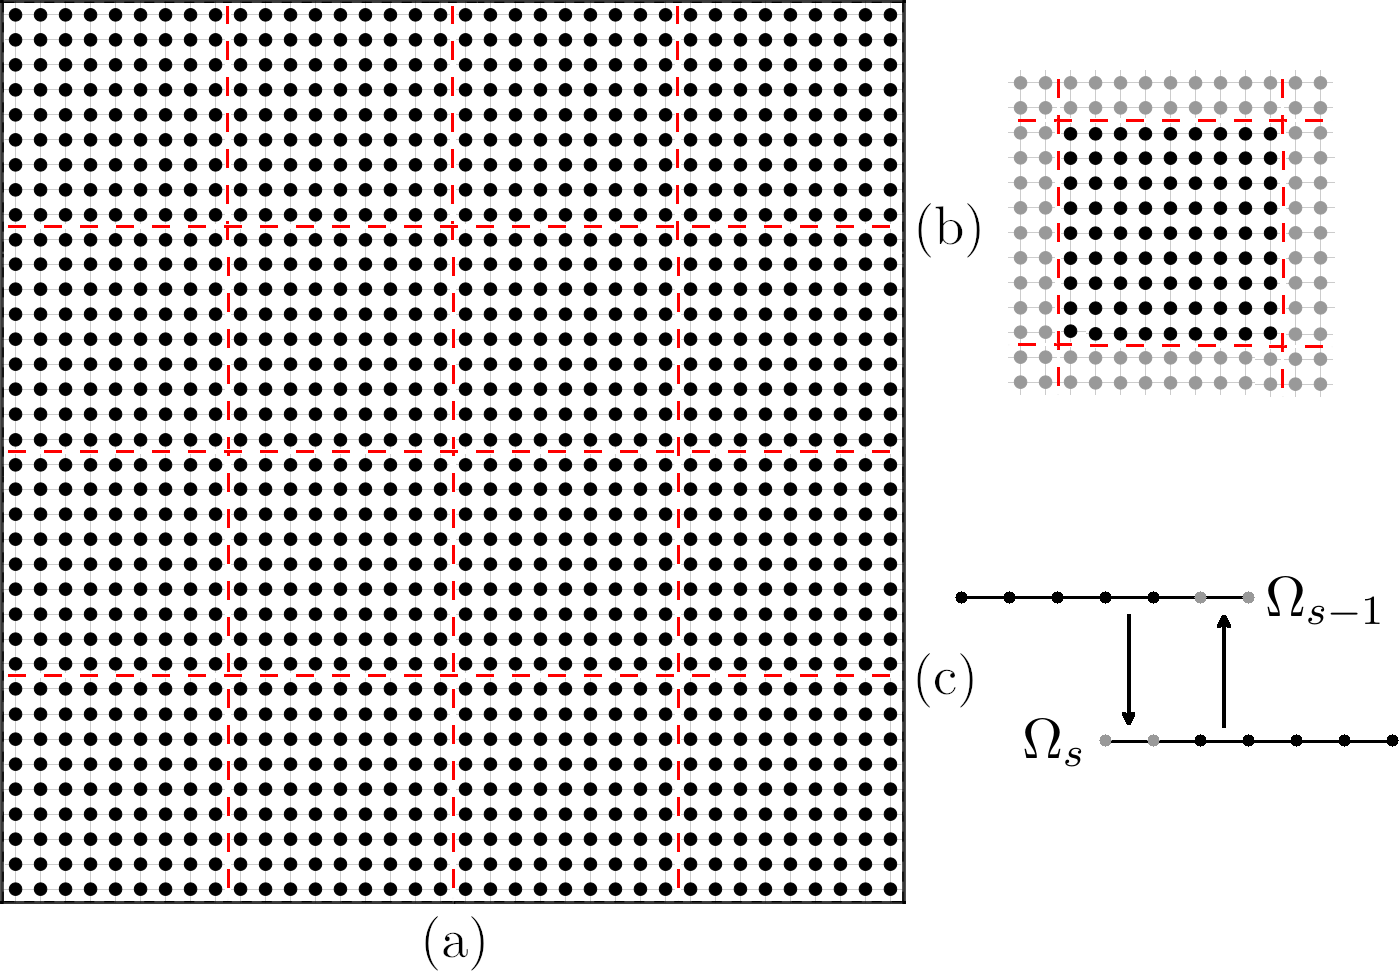
\includegraphics[width=0.6\linewidth]{figuras/all.png}
  \caption{a) El dominio $\Omega$ es dividido en subdominios disjuntos $\widetilde{\Omega}_s$ de modo que 
   $\Omega=\cup_{s=1}^{N_{c}}\widetilde{\Omega}_s$.
   b) Cada subdominio $\widetilde{\Omega}_s$ es extendido  
  en dos puntos (círculos grises) en cada dirección espacial, formando una descomposición en 
  subdominios solapados $\Omega_s$, los cuales se superponen con los subdominios vecinos 
  de forma que $\Omega=\cup_{s=1}^{N_{c}}\Omega_s$. 
  En esta región se recibe información de subdominios vecinos.
   c) Intercambio de información en los bordes de los subdominios solapados 
    $\Omega_s$ y $\Omega_{s-1}$. El 
   procesador $s$ envía a su vecino $s-1$ la información del tercer y cuarto punto de la grilla $s$, y 
   recibe de su vecino los primeros dos puntos.}
 \label{fig:bechange}
\end{figure}

 Cada subdominio contiene un conjunto de puntos  $x_s\in[x_{\text{min},s},x_{\text{max},s}]$ 
 y $y_s\in [y_{\text{min},s},y_{\text{max},s}]$, con los puntos 
 en la grilla dados por $x_i=x_{\min,s}+(i-1)\Delta x$ e $y_j=y_{\min,s}+(j-1)\Delta y$. 
 Definimos  $u_{m}^k(x,y_j)\equiv u_{m,j}^k(x)$ la intensidad específica discretizada a tiempo $t^k$, 
 en la dirección $\hth_m$,
  donde se fijó $y_j\in y_s$ para cualquier $x\in x_s$. 
  Similarmente definimos $u_{m}^k(x_i,y)\equiv u_{m,i}^k(y)$. Al final de cada paso temporal, 
 se realiza el intercambio de puntos entre subdominios vecinos para todos los bordes que no son físicos (bordes 
 originados por la partición), 
 para cada proceso, en cada dirección espacial, y para cada punto de la grilla 
 en esa dirección, como se ilustra en la Figura (\ref{fig:bechange}).

En suma, el algoritmo que resulta de la combinación del método FC con 
el método de ordenadas discretas (D.O.M., del inglés discrete ordinates method), y el método de propagación temporal, 
lo denominamos método FC--DOM~\cite{Gaggioli2019}. El pseudocódigo se presenta en el algoritmo~\eqref{algfc}.
\begin{algorithm}[H]
\caption{FC--DOM en paralelo}\label{algfc}
\begin{algorithmic}[1]
\State  Generar descomposición de dominio
\State Asignar un subdominio $\Omega_s$ a cada procesador.
\State \textbf{para} cada $\Omega_s$ \textbf{hacer} en paralelo
\State \hskip0.5em  Asignar vectores iniciales para el esquema de Adams--Bashforth.
\State \hskip0.5em \textbf{para} cada paso temporal k \textbf{hacer}
\State \hskip0.75em \textbf{para} Cada dirección $\hth_m$ \textbf{hacer} \emph{}
\State \hskip1.0em \textbf{para} cada $y_j$ \textbf{hacer} en la dirección $\hat x$
\State \hskip1.5em Aplicar la continuación de Fourier a $u_{m,j}^k(x)$.
\State \hskip1.5em Aplicar la Transformada Rápida de Fourier para obtener eq.~\eqref{eq:RTEFCSum}.
\State \hskip1.5em Evaluar $\partial u_{m,j}^k(x)/\partial x$ usando la ec.~\eqref{eq:RTEFCSumder}.
\State \hskip1.0em\textbf{terminar}
\State \hskip1.0em\textbf{para} cada $x_i$ \textbf{hacer} en la dirección $\hat y$ 
\State \hskip1.5em Aplicar la continuación de Fourier a $u_{m,i}^k(y)$.
\State \hskip1.5em Aplicar la Transformada Rápida de Fourier para obtener eq.~\eqref{eq:RTEFCSum}.
\State \hskip1.5em Evaluar $\partial u_{m,i}^k(y)/\partial y$ usando ec.~\eqref{eq:RTEFCSumder}.
\State \hskip1.0em\textbf{terminar}
\State \hskip1.0em Evaluar el lado derecho de la ec.~\eqref{eq:RTEAB4}.
\State \hskip1.0em Imponer condiciones de borde.
\State \hskip1.0em Intercambiar bordes no físicos entre subdominios vecinos.
\State \hskip0.75em\textbf{terminar}
\State \hskip0.5em\textbf{terminar}
\State  \textbf{terminar}
\end{algorithmic}
\end{algorithm}
Para realizar un estudio de escalabilidad proponemos un problema típico, 
con  $N=2000$ puntos en cada coordenada espacial $M=16$ direcciones, 
y $T=1000$ pasos temporales. 
Se utilizó un cluster con procesadores Intel Xeon E5-2630 v3 at 2.40GHz de 24 núcleos físicos 
y 128Gb de memoria RAM por nodo. Esta máquina implementa la tecnología ``Intel turbo'', 
que acelera el desempeño del procesador dependiendo de la carga de trabajo y el entorno operativo. 
Para realizar un análisis correcto de escalabilidad, y balancear apropiadamente 
la carga de los nodos, utilizamos 16 procesadores por nodo, 
comparando los tiempos computacionales entre 1 y 16 nodos. 
En la Figura \ref{fig:scala} se observan los tiempos de cómputo 
normalizados $t^*=t/t_{16}$ con respecto al tiempo de cómputo 
en 16 procesadores. 
Como se observa, el algoritmo 
propuesto presenta \textit{escalabilidad paralela perfecta} 
hasta los 256 procesadores para los que fue probado. 
\begin{figure}[h!]
\centering
  \includegraphics[width=0.5\linewidth]{figuras/escalabilidad.eps}
  \caption{Estudio de escalabilidad para problema modelo. 
  Círculos rojos: escalabilidad perfecta, para 256 procesadores $1/t^*=16$. 
  Diamantes negros: Escalabilidad obtenida, $1/t^*=21.872$, dando 
 una eficiencia de $136.7\%$.}
 \label{fig:scala}
\end{figure}

La razón por la cual la escalabilidad obtenida es supralineal se 
desarrolla ampliamente en el trabajo de Albin y Bruno~\cite{Albin2011}
(sección 6). Esencialmente, esto se debe a que el 
las transformaciones FFT 
poseen una complejidad computacional $\mathcal{O}(N\log(N))$.

\section{Validación}

Dado que los algoritmos y los códigos utilizados han sido desarrollados 
originalmente en este trabajo, ha sido necesario realizar exhaustivas 
pruebas de convergencia y validación. Para ello, 
hemos corroborado nuestros resultados tanto con valores experimentales 
como con soluciones analíticas reportadas en la literatura.

\subsection{Convergencia de soluciones manufacturadas}
\label{sec:manufacturada}

Para mostrar las propiedades de convergencia del algoritmo propuesto,
estudiamos un problema manufacturado, analizando el error generado en la propagación de 
la solución.
Con este fin, resolvemos el problema ETR dado por 
\begin{equation*}
\begin{split}
\begin{aligned}
&\frac{1}{c}\frac{\partial }{\partial t}\ut + \hth \cdot \nabla \ut+a(\x)\ut  \\
&\quad \quad \quad  \quad \quad \; \;\,  +b(\x)\ut = \int_{S^1}\eta(\hth\cdot\hth ') 
u(\x,\hat \theta',t) d\theta'+s(\x,\hth,t),  \; (\x,\hth)  \in \Omega\times S^1\\
&u(\x,\hth,t=0)=u_0, \; (\x,\hth)  \in \Omega\times S^1,  \\
&u(\x,\hth,t)=u_b, \; (\x,\hth) \in \Gamma_-. \notag
\end{aligned}
\end{split}
\label{eq:RTEdisp}
\end{equation*}
para $0\leq t \leq T$. 

Proponemos la solución manufacturada
\begin{equation*}
u^{\text{an}}(\x,\hth,t)=e^{-(x-t)^2-(y-t)^2-\cos(\theta)^2}.
\label{eq:RTEmansol}
\end{equation*}
donde el término de la fuente $s(\x,\hth,t)$, 
la condición inicial $u_0(\x,\hth,t)$ y las condiciones 
de contorno $u_b(\x,\hth,t)$ en la ecuación~\eqref{eq:RTEdisp} 
se obtienen, respectivamente, aplicando el operador de transporte, 
evaluando a tiempo $t=0$ y en $\Gamma_-$ la solución manufacturada 
propuesta~\eqref{eq:RTEmansol}.
Resolvemos el problema~\eqref{eq:RTEdisp} en un dominio cuadrado 
$\Omega=\{ \x \in [x_{\text{min}},x_{\text{max}}]\times [y_{\text{min}},y_{\text{max}}] \}$
donde $x_{\text{min}}=y_{\text{min}}=0$ cm, $x_{\text{max}}=y_{\text{max}}=3$ cm, 
y evolucionamos la solución hasta el tiempo final $T=3$ ps. Utilizamos 
una descomposición de 8 subdominios para 
poder realizar estas pruebas en una PC de escritorio. 
El coeficiente de dispersión en el medio considerado es isótropo, 
con $g=0$, $a(\x)=0.35/$cm y $b(\x)=20/$cm. 
%\pagebreak

Evaluamos el error máximo obtenido en todo el dominio 
comparando el flujo escalar dado por la ecuación~\eqref{eq:photondensity} 
obtenido numéricamente comparado con el obtenido analíticamente
\begin{equation*}
\begin{split}
\begin{aligned}
\phi^{\text{an}}(\x,t)&=\int_{2\pi} u^{an}(\x,\theta,t) d\theta=
k_{\phi}\times e^{-(x-t)^2-(y-t)^2},\\
k_{\phi}&=\int_{2\pi}e^{-\cos(\theta)^2}d\theta\simeq 4.0528...,
\end{aligned}
\end{split}
\label{eq:photondensityan}
\end{equation*}
y estudiamos las propiedades de convergencia 
para todas las variables involucradas. La constante 
$k_{\phi}$ se calcula con 16 dígitos de precisión. 
La solución numérica es evaluada hasta el tiempo final $T$, 
y luego se calcula el error máximo según
\begin{equation*}
\varepsilon=\text{max}_{\x \in \Omega} |\phi^{\text{num}}(\x,T) -\phi^{\text{an}}(\x,T)|.
\label{eq:maximumerror}
\end{equation*}
El error numérico es en general una función 
de cada una de las variables discretizadas en la ETR, 
\ie~$\varepsilon=\varepsilon(\Delta \x, \Delta \theta, \Delta t)$. 
Al comparar el término del error para una grilla de una dada variable, 
el resto de los parámentros de discretización permanecen fijos.
\begin{wrapfigure}{r}{0.45\textwidth}
 \begin{subfigure}{
  \includegraphics[width=0.45\textwidth]{figuras/errdt.eps}}
 \end{subfigure}
 \begin{subfigure}{
  \includegraphics[width=0.45\textwidth]{figuras/errdx.eps}}
 \end{subfigure}
 \begin{subfigure}{
  \includegraphics[width=0.45\textwidth]{figuras/errdm.eps}}
 \end{subfigure}
  \caption{Convergencia del algoritmo FC--DOM en paralelo 
  para cada una de las variables en la ETR. Las líneas rectas discontinuas 
  muestran la pendiente para un orden de convergencia prescripto. }
 \label{fig:convman}
\end{wrapfigure}

El alto orden de convergencia del algoritmo FC--DOM en paralelo 
para la solución manufacturada propuesta se muestra en la figura~(\ref{fig:convman}). 
Esta convergencia es la esperada dadas las aproximaciones 
numéricas empleadas.
%\pagebreak 
%\clearpage
\subsection{Comparación con resultados experimentales}
\label{sec:resexp}

En esta sección comparamos los resultados producidos por el algoritmo FC--DOM 
con resultados experimentales obtenidos para varios 
medios similares al tejido humano, realizados por Klose \textit{et al.}~\cite{Klose2002}. 
En las mediciones reportadas en dicha referencia, 
se utilizan fantomas compuestos de resina epoxy y tinta, 
con una concentración de monoesféras de dióxido de silicio ($\text{SiO}_2$). 
La tinta permite ajustar la absorción óptica del fantoma, 
mientras que las monoesféras de silicio determinan su dispersión. 
Las propiedades ópticas del medio (los coeficiente de absorción $a(\x)$
y dispersión $b(\x)$ y el 
factor de anisotropía $g$) han sido determinadas por Klose \textit{et al.} mediante 
diferentes métodos independientes. Estos incluyen simulaciones de Monte--Carlo, 
la técnica de esfera integradora, aproximación de difusión, y teoría de 
dispersión de Mie para ondas electromagnéticas. 

La aproximación de difusión, ampliamente utilizada en tomografía óptica para el 
modelado de transporte de fotones en el tejido biológico, 
es válida para medios de alta dispersión,  
baja absorción y en regiones alejadas de las fuentes.
Dado que nuestro método resuelve el problema ETR completo, podemos considerar adecuadamente 
medios con baja absorción y dispersión, como puede ser el fluido cerebroespinal 
en la cabeza, o la traquea en un cuello humano. 

Analizaremos dos arreglos experimentales diferentes propuestos por Klose~\textit{et al.}. 
Estos poseen simetría 2D, apropiada para nuestro tratamiento. 
 En el primer experimento, se simula un cubo homogéneo, de propiedades ópticas dadas en 
 la Tabla~\ref{tab:tabopt}.
 En el segundo, la geometría del fantoma también 
 es cubica, pero contiene una inhomogeneidad en forma 
 de anillo cilíndrico, con agua en su interior. Esta inhomogeneidad 
 es similar a la que se encuentra en 
 el fluido cerebroespinal, y el fantoma constituye un modelo 
 simple para una cabeza humana. En ambos experimentos,
los fantomas fueron iluminados con luz láser en el 
infrarrojo ($\lambda = 678$ nm), en tres posiciones a lo largo del eje $x$. Se detectó la luz emergente 
en dos de las caras de los fantomas, como se muestra en la figura~(\ref{fig:phantom}).

 
 \begin{table}[h!]
\caption{Propiedades ópticas de los fantomas}
\vspace{-0.6cm}
\begin{center}
\begin{tabular}{cccc}
\hline
$\mu_s$ $[cm^{-1}]$ ~~~~~~~~ & $\mu_a$ $[cm^{-1}]$ & ~~~~~~~~ $g$  ~~~~~~~~ & $n_{\Omega}$ \\
\hline
58 ~~~~~~~~ & 0.35 & ~~~~~~~~  0.8 ~~~~~~~~ & 1.56 \\
\hline
\end{tabular}
\label{tab:tabopt}
\end{center}
\end{table}

\begin{figure}[h!]
\centering
  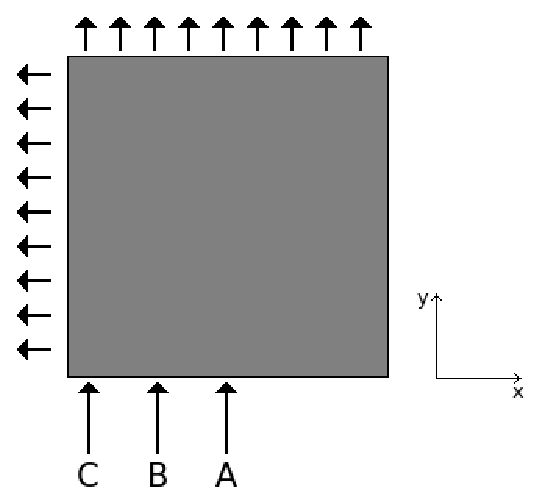
\includegraphics[width=0.4\linewidth]{figuras/phantom.eps}
   \caption{Arreglo experimental de Klose \textit{et al.}~\cite{Klose2002}. 
   Las flechas apuntando hacia el fantoma (A, B y C)  
   muestran las tres posiciones diferentes en las que se inyectó 
   la luz láser. Las flechas salientes muestran las posiciones de los detectores 
   con las que se midió la radiación saliente.}
 \label{fig:phantom}
\end{figure}

El método de continuación de Fourier extiende 
la intensidad específica en el borde del dominio, 
permitiendo el tratamiento de condiciones de borde generales y no periódicas.  
Esto previene el surgimiento del fenómeno de Gibbs debido a la no periodicidad 
de la función. La fuente $q(\x,\hth,t)$ y los parámetros ópticos 
también pueden dar origen al fenómeno de Gibbs si no son 
tratados correctamente. Los problemas numéricos que surgen 
debido a discontinuidades son resueltos mediante aproximaciones arbitrariamente precisas 
introduciendo funciones suaves que presentan 
variaciones rápidas en la región de discontinuidad (en conjunto 
con discretizaciones capaces de resolver dichas variaciones).

Dado que nuestro algoritmo resuelve el problema ETR dependiente del tiempo, 
y que los resultados experimentales reportados por Klose \textit{et al.} 
son independientes del tiempo, evaluaremos la corriente de fotones saliente 
\begin{equation}
 \vec{ \mathcal{J}}_+(\x,t)=\int_{\Gamma_+} [1-f(\hth \cdot \hnu)] \hth \cdot \hnu u(\x,\hth,t) d\theta,
\label{eq:photoncurrentsal}
\end{equation}
utilizando una función sigmoidea para el perfil temporal, $T(t)$, 
que adquiere suavemente valores partiendo desde cero 
hasta uno. La solución independiente del tiempo 
se adquiere a un tiempo asintótico.
La fuente láser se modela por la función
\begin{equation}
q(\x,\hth,t)=T(t)\exp \left(  -\frac{|\x-\x_s|^2}{2\sigma^2} \right)  \, ,
\label{eq:sourceGauss}
\end{equation}
donde el valor de $\sigma=0.1$ cm es el reportado para el experimento y $\x_s$ 
representa la posición del láser. La información direccional de la fuente 
puede ser muy valiosa en diversos tipos de experimentos. 
En el caso particular que analizamos, el medio es altamente dispersivo. Por lo tanto, los 
fotones pierden rápidamente esta información 
luego de atravesar una corta distancia (del orden del camino libre medio).

Se resuelve la ETR para un número de pasos temporales, 
hasta que la solución alcanza, numéricamente, el comportamiento 
asintótico~\cite{Bruno2010}, para el cual $\lim_{t\to \infty} \frac{\partial u}{\partial t}=0$. 
Luego se evalúa el operador de la ecuación~\eqref{eq:photoncurrentsal} 
en las regiones de la superficie en $\partial \Omega$ 
donde se ubican los detectores.
Una vez  calculada la corriente de fotones salientes, se
se realiza una normalización para ubicar la lectura 
de los resultados experimentales (reportados en escala arbitraria) 
en la misma escala que las obtenidas por el método FC--DOM. 
Para las detecciones a lo largo del eje $x$ se normalizó 
con respecto al máximo valor de cada curva. 
 Las lecturas de los detectores sobre el eje $y$ 
 se normalizaron ajustando el punto en la grilla numérica 
 que se encontró mas cerca de la posición reportada 
 para alguno de los detectores. 
 
\subsubsection{Fantoma homogéneo}

El primer arreglo experimental reportado por~\cite{Klose2002} 
se basa en un fantoma homogéneo con los parámetros ópticos 
dados en la tabla~\ref{tab:tabopt}. El fantoma posee un tamaño  
de $3$ cm a lo largo de los ejes $x$ e $y$. La posición del láser 
   $\x_s$ es, para los tres casos considerados $A=(1.5,0)$ cm, $B=(0.9,0)$ cm
    y $C=(0.3,0)$ cm. En la figura~(\ref{fig:ph1timef}) se muestra 
el flujo escalar~\eqref{eq:photondensity} 
correspondiente a las tres posiciones de la fuente láser $\x_s$. 

\begin{figure}[h!]
\centering
  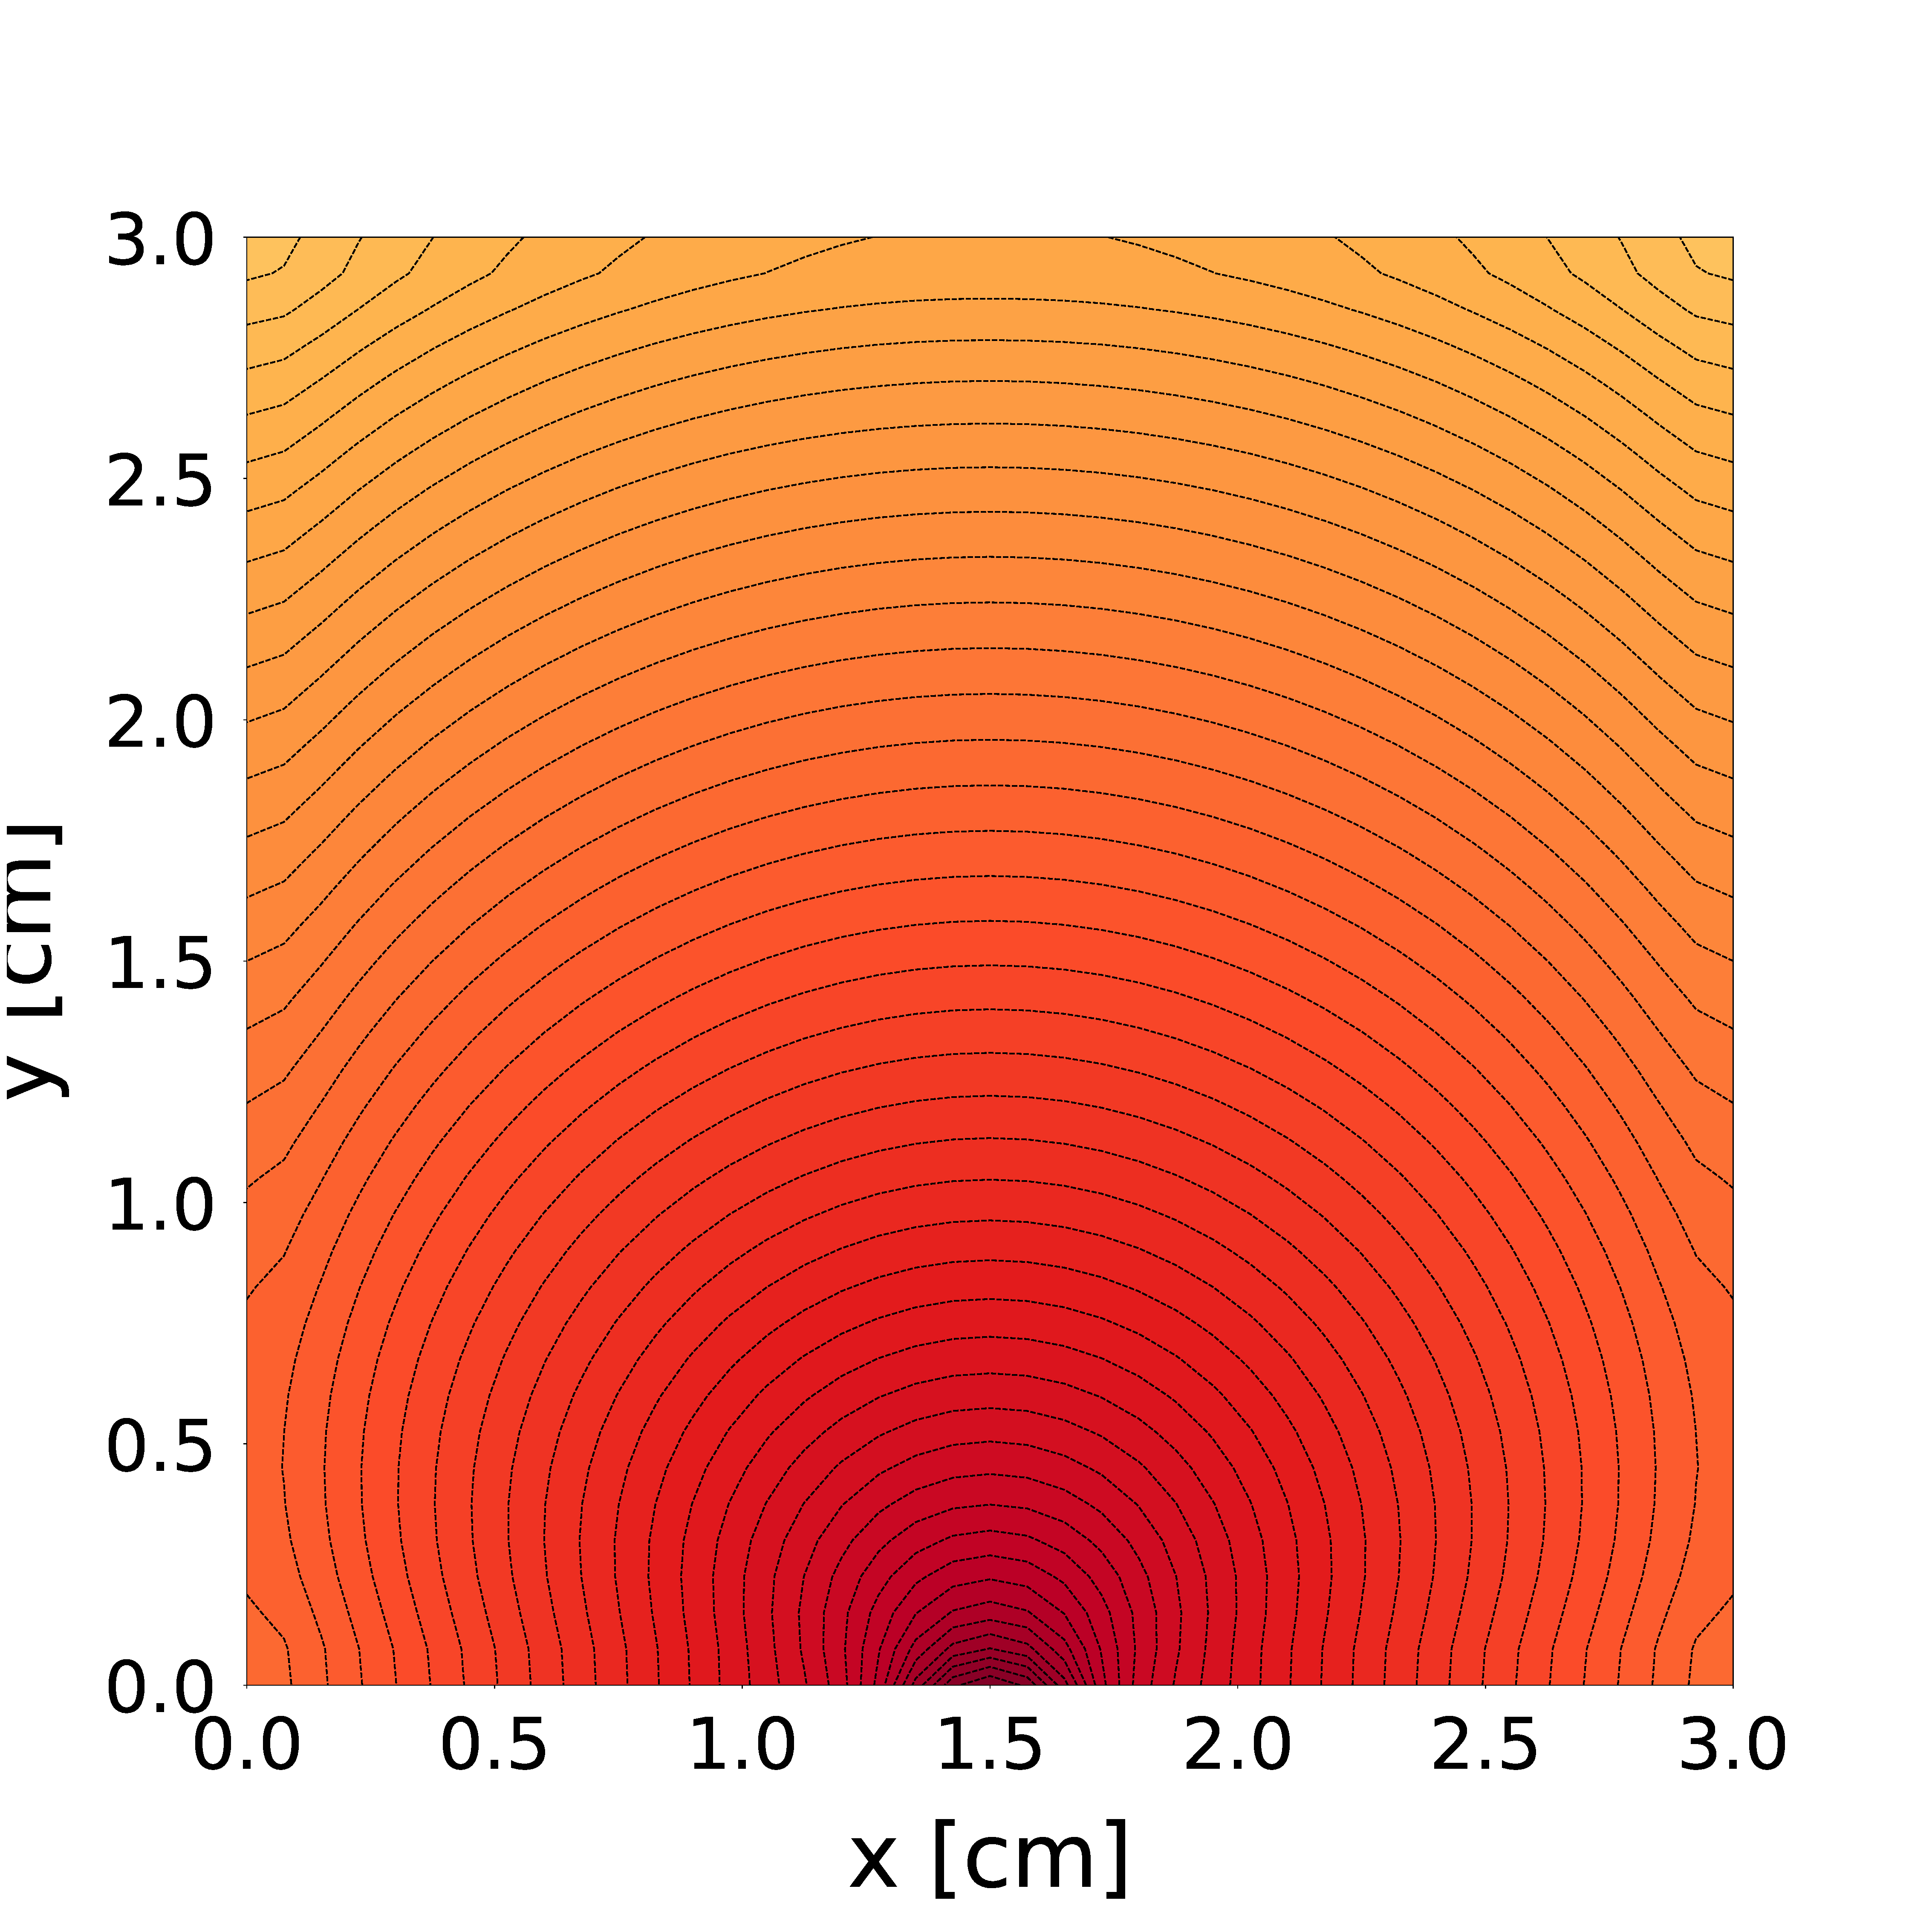
\includegraphics[width=0.32\linewidth]{figuras/ph1A.eps}
  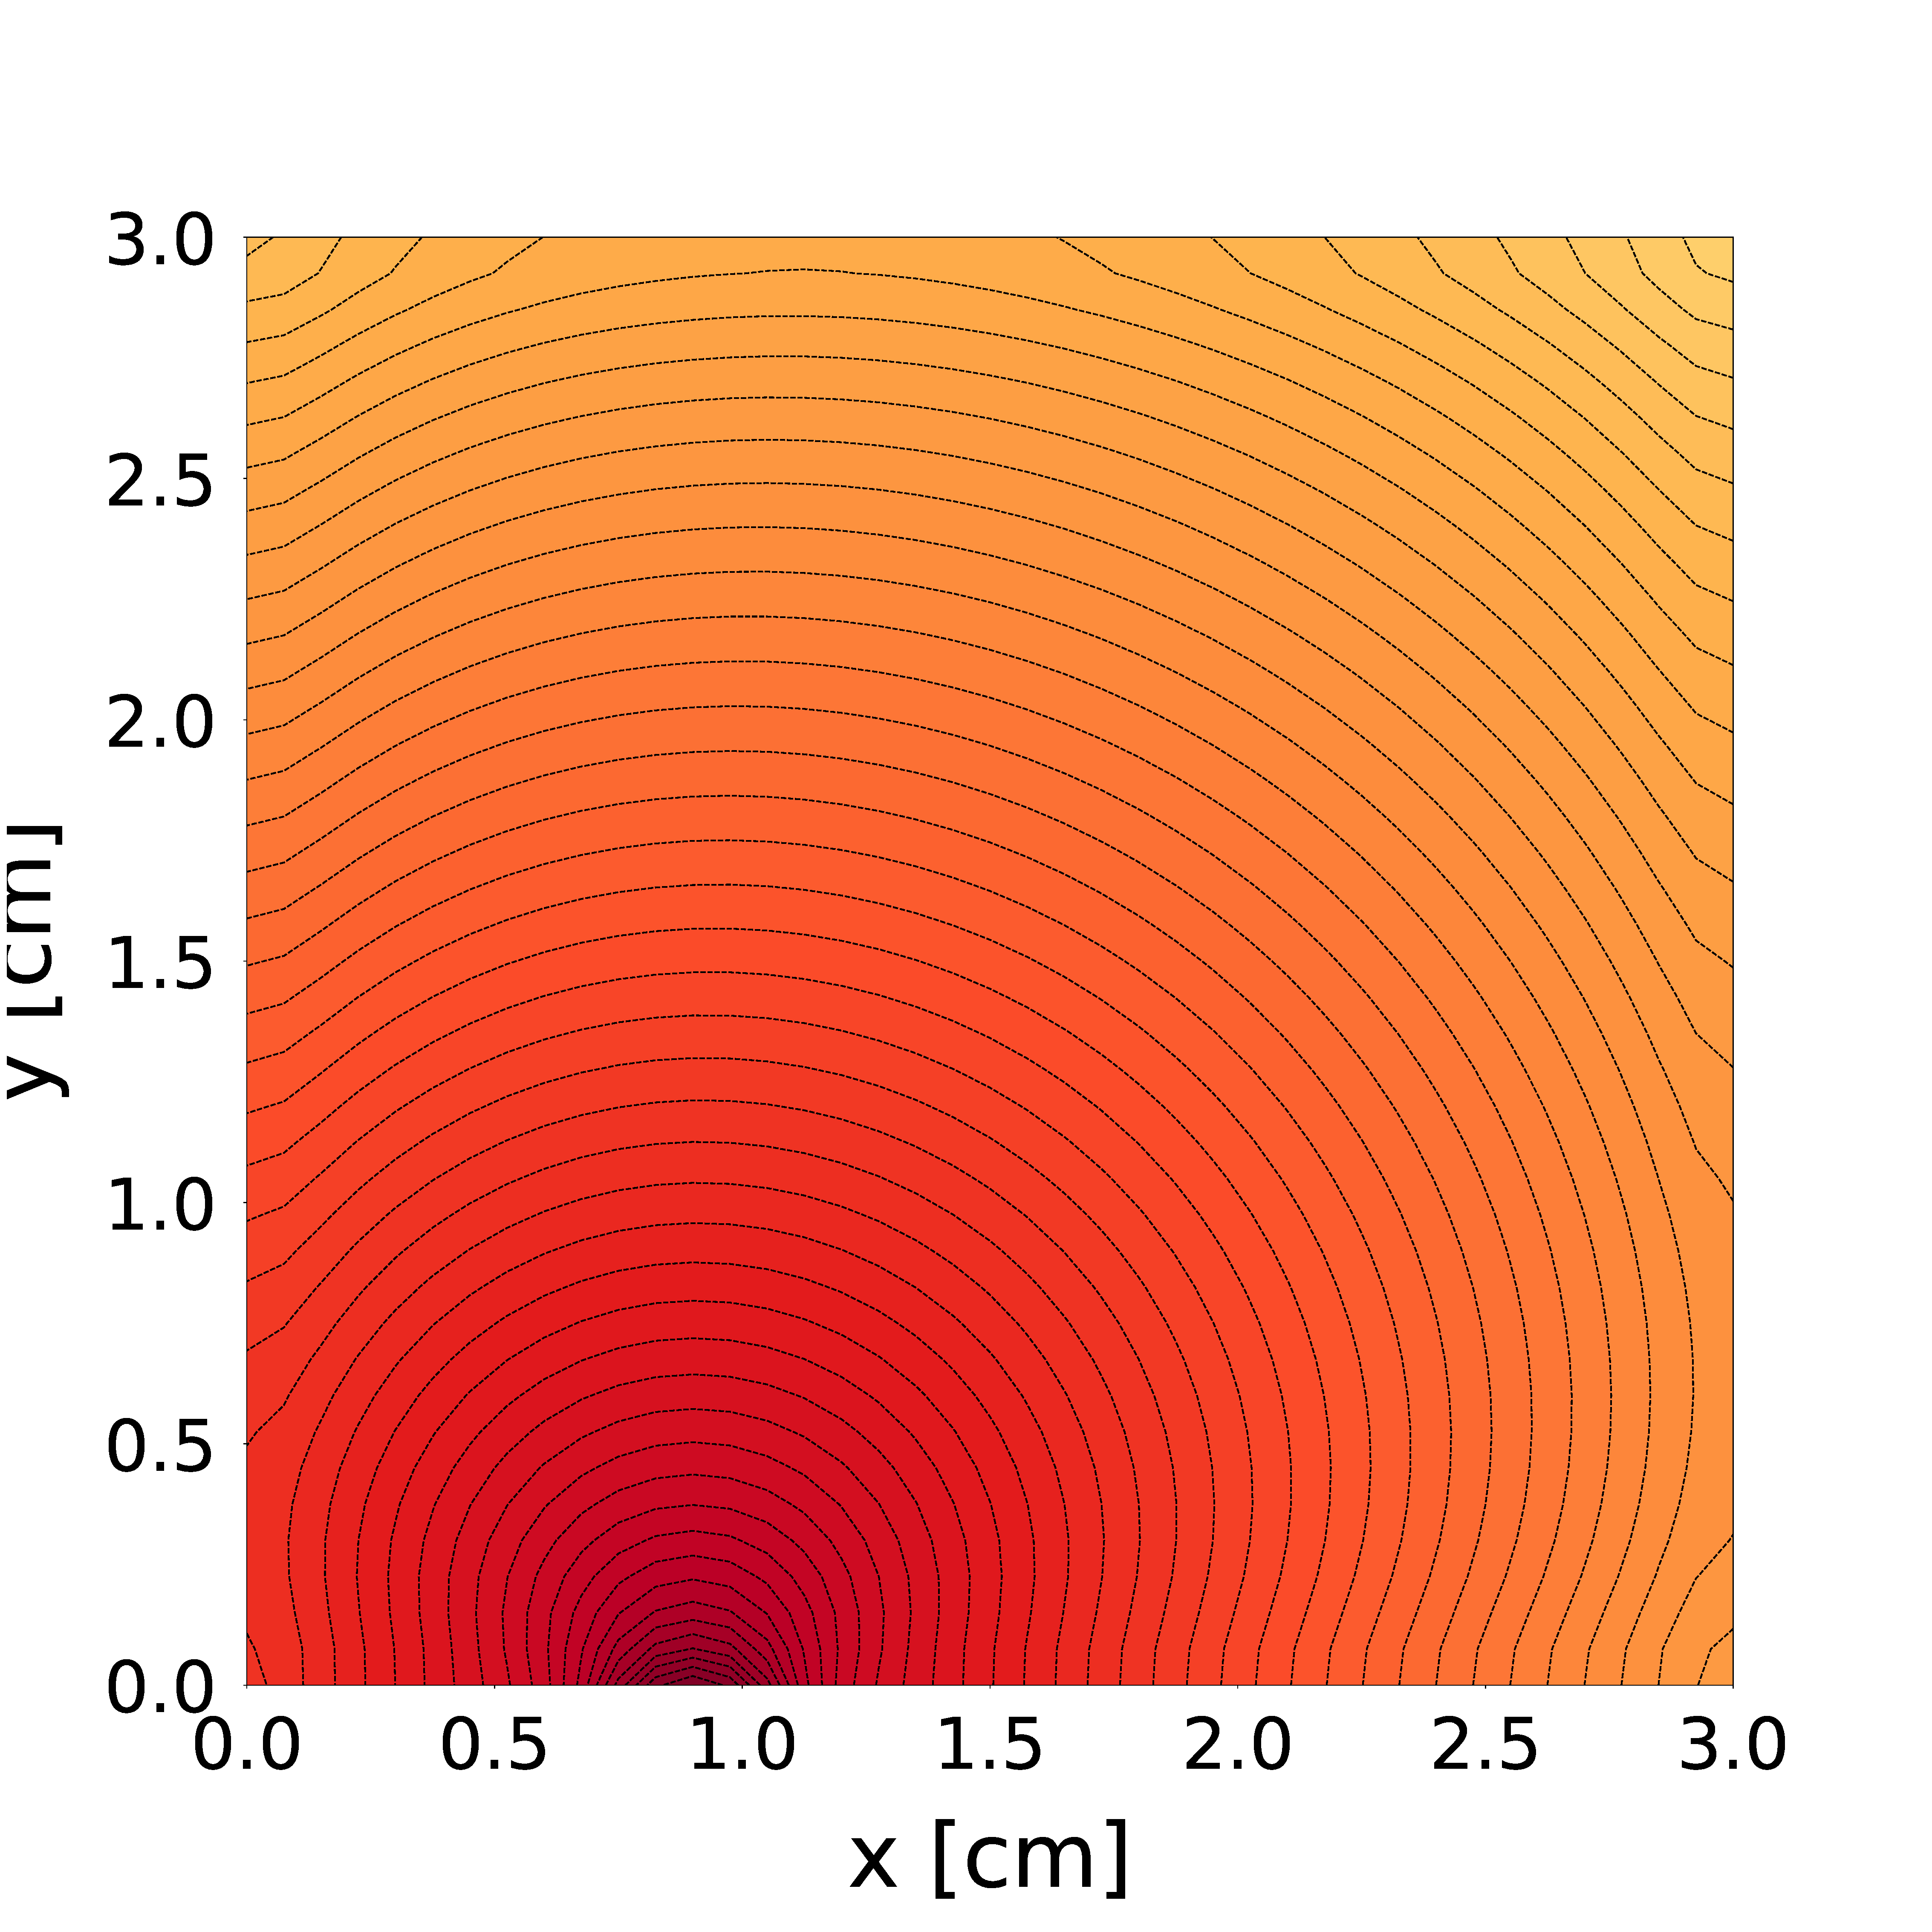
\includegraphics[width=0.32\linewidth]{figuras/ph1B.eps}
  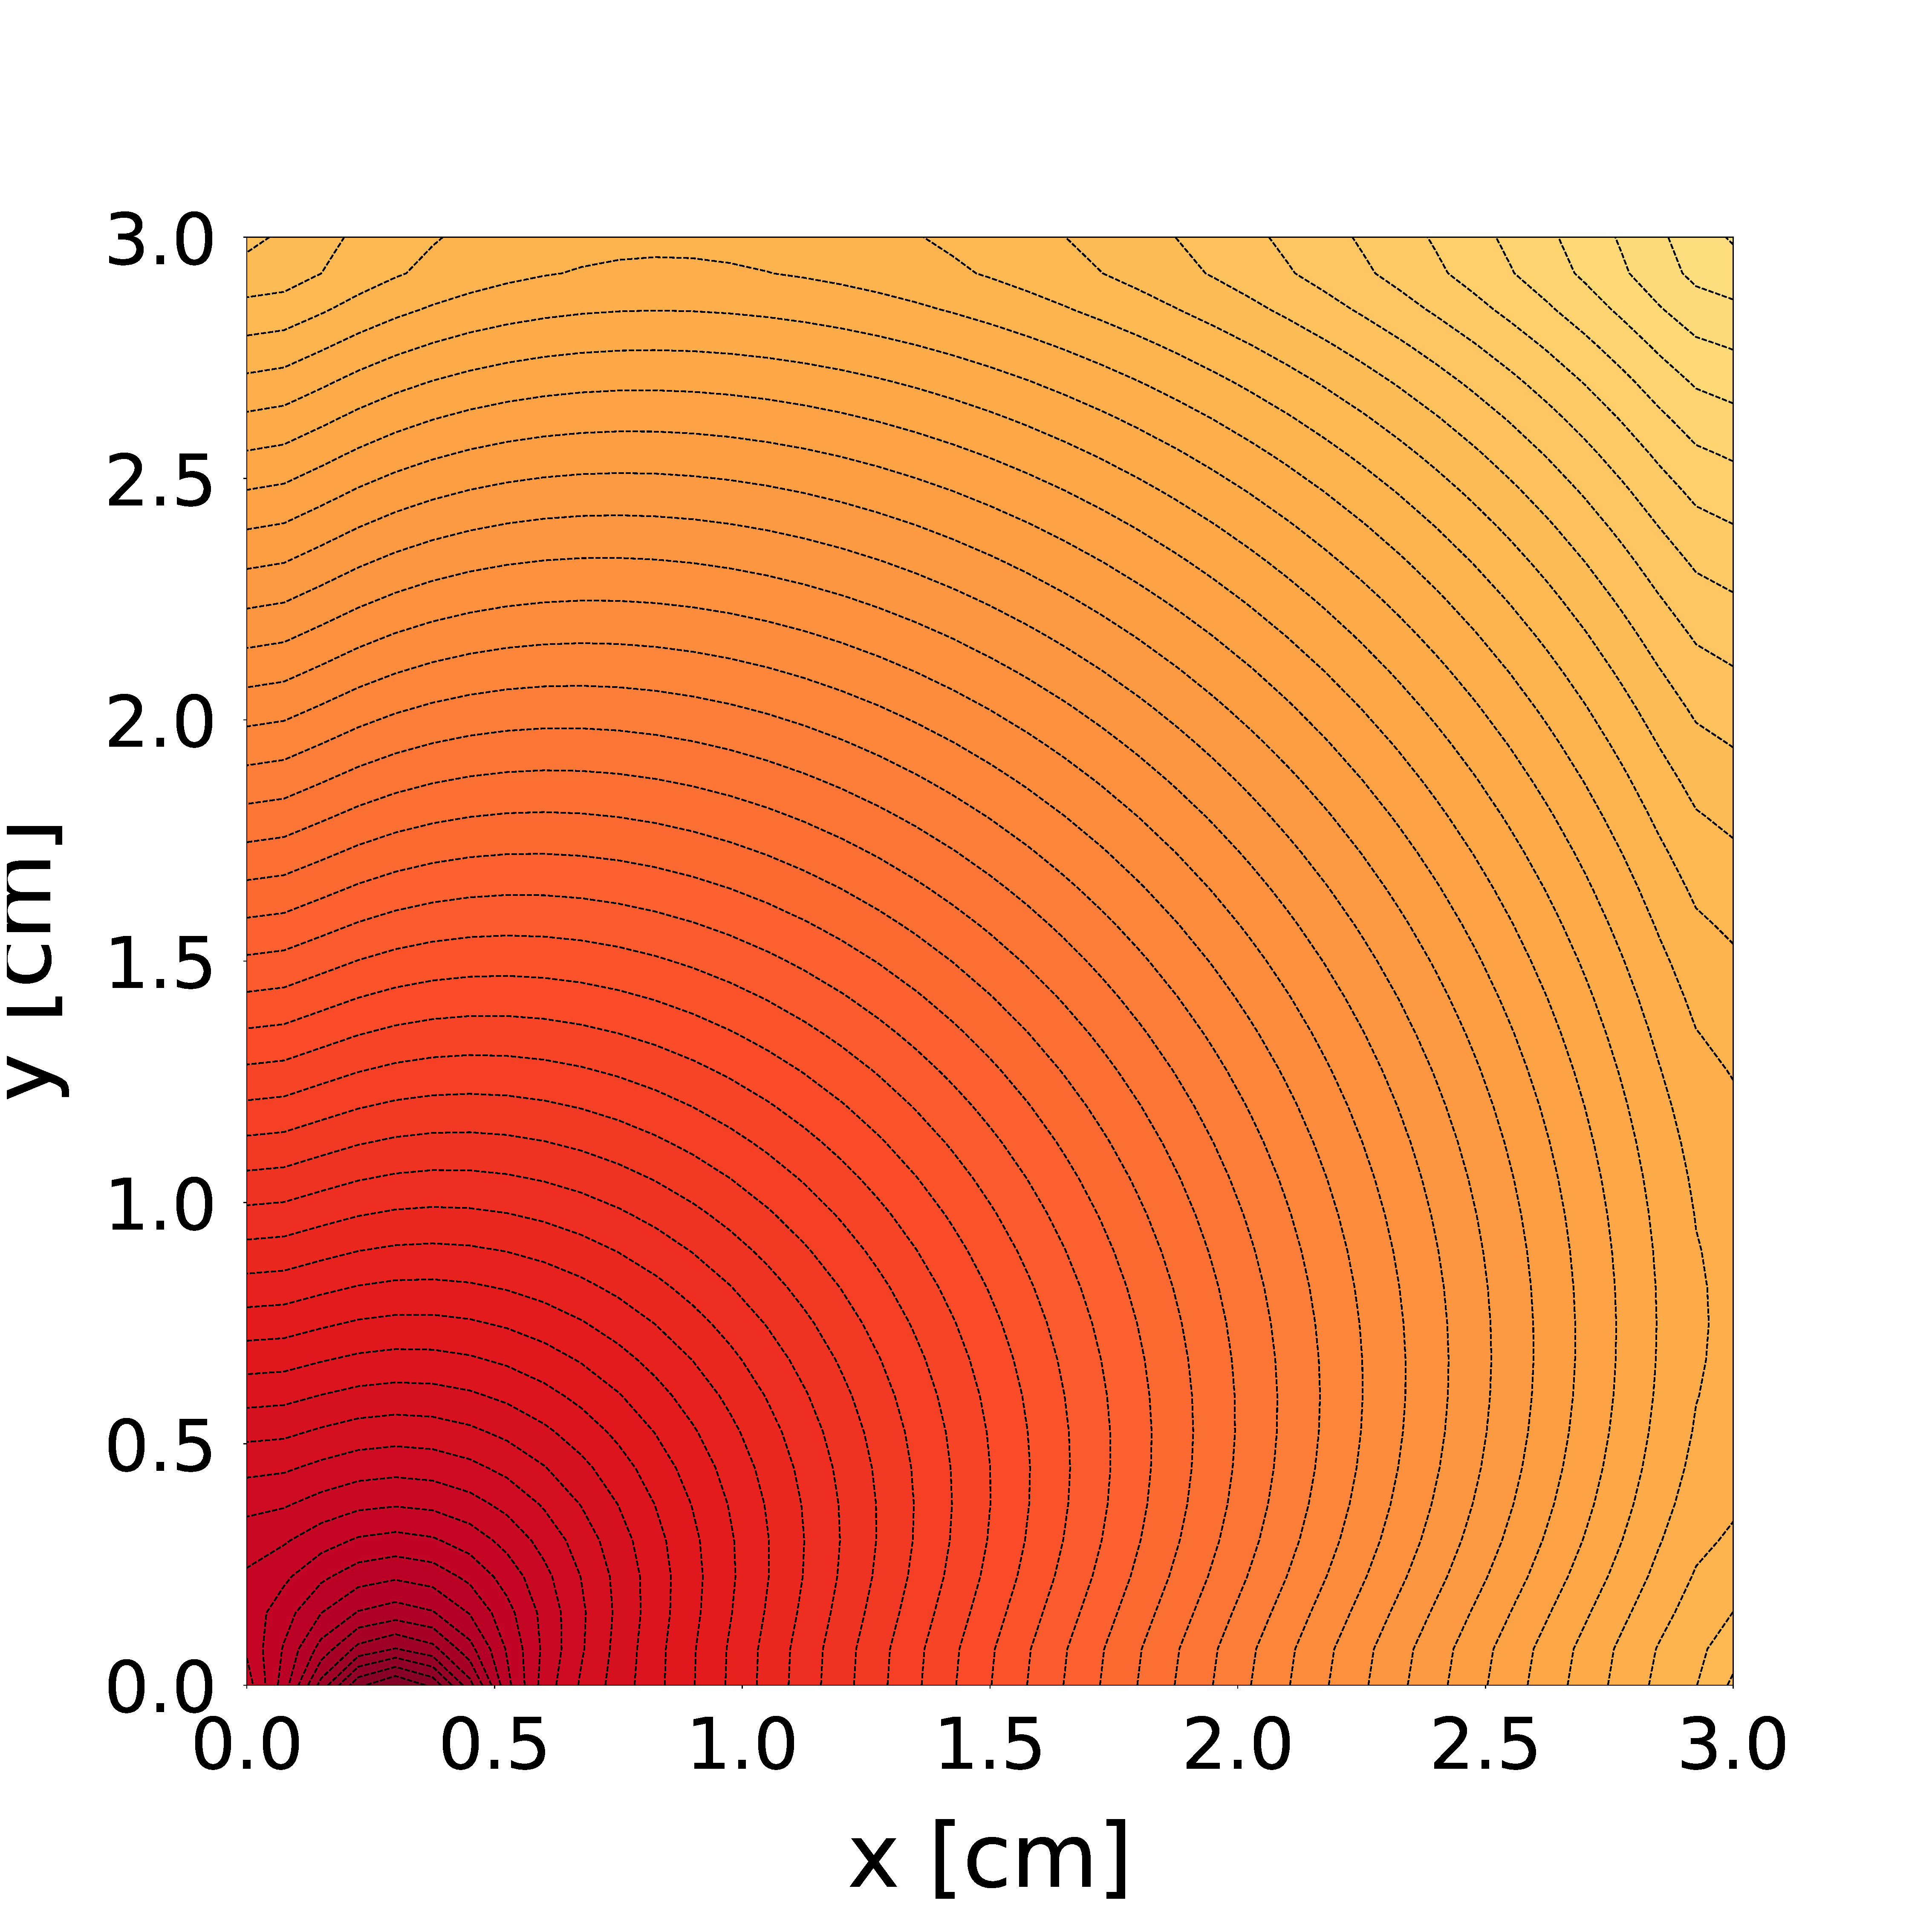
\includegraphics[width=0.32\linewidth]{figuras/ph1C.eps}
  \caption{
  Flujo escalar $\phi(\x)$~\eqref{eq:photondensity} 
  obtenido en la simulación para el fantoma homogéneo. 
  Las tres figuras muestran los resultados obtenidos 
  para las fuentes ubicadas en A (izquierda), B (centro) y C (derecha). 
  Debido al decaimiento exponencial inherente a la solución, 
  la figura se presenta en escala logarítmica para apreciar los detalles.}
\label{fig:ph1timef}
\end{figure}
Como puede apreciarse en la figura, el flujo escalar para el caso A 
es simétrico con respecto al eje vertical situado en la posición 
de la fuente, pero el sistema pierde esta propiedad cuando la 
posición de la fuente se ubica más cerca de los bordes, 
dando lugar a reflexiones que afectan la intensidad 
de la luz con una dependencia angular particular.

El flujo de fotones que llegan a los detectores, ubicados en el borde $\partial \Omega$ 
del dominio, se obtuvo mediante la ecuación~\eqref{eq:photoncurrentsal}. 
Los resultados se muestran en la Figura~(\ref{fig:fluxph1}), 
para los 28 detectores ubicados en el borde a lo largo del eje $x$ (izquierda) 
y para los 28 detectores en la dirección $y$ a la derecha. 
Se observa un acuerdo excelente entre los resultados simulados (líneas) 
y los datos experimentales (en símbolos).  El máximo 
flujo de fotones salientes $\mathcal{J}_+$ en los experimentos B, 
y particularmente en el C, se encuentran desviados con respecto a la posición 
de la fuente láser. Esto puede explicarse considerando la radiación 
que está siendo reflejada y que escapa a través de la superficie de la izquierda. 
A medida que la fuente se acerca más al borde, el ángulo de incidencia de la 
radiación con respecto a la normal de la superficie aumenta. Por lo tanto, 
más radiación resulta reflejada desde puntos cercanos a la superficie, 
propagandose hacia el interior del medio participante, 
contribuyendo al máximo. También se espera que la contribución de fotones dispersados 
por el medio desde la región a la derecha sea relativamente mayor 
que desde la izquierda, ya que la radiación 
dispersada en esta última tiende a escapar por el borde. 
\begin{figure}[h!]
\centering
  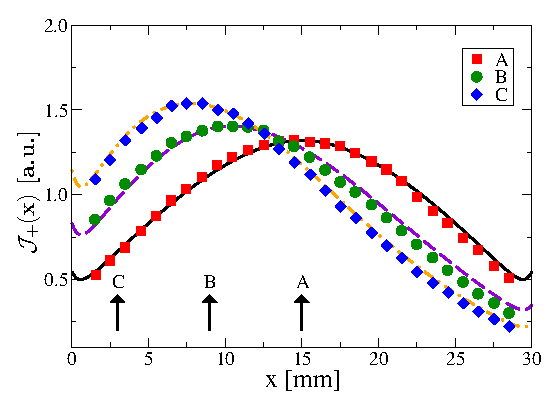
\includegraphics[width=0.48\linewidth]{figuras/kloseph1x.eps}
  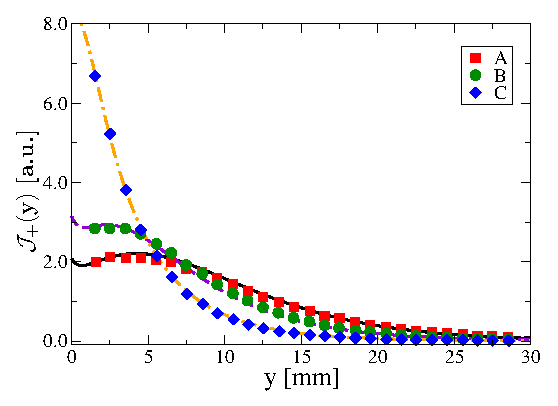
\includegraphics[width=0.48\linewidth]{figuras/ph1y.eps}
  \caption{Radiación transmitida medida por Klose~\cite{Klose2002} (símbolos), 
  y simulada mediante el método FC--DOM (lineas) para el fantoma homogéneo. }
 \label{fig:fluxph1}
\end{figure}
También puede observarse un aumento en el flujo de fotones en la región más 
cercana al borde, proveniente de fotones que han sufrido reflexión total interna.

Este experimento también fue simulado y analizado por Klose {\it et al.}~\cite{Klose2002}
en el marco de la teoría ETR independiente del tiempo.

\subsubsection{Fantoma inhomogéneo}

El segundo fantoma contiene una región de ``vacío'' en forma de anillo, 
rellena de agua, de diámetro $d=2,8$ cm, en donde el coeficiente de absorción 
y dispersión están dados por $\mu_a=\mu_s=0$. En el resto del medio, 
se consideran los parámetros ópticos de la tabla~\ref{tab:tabopt}
Las dimensiones de este fantoma a lo largo del eje $x$ e $y$ es de $4$ cm.
Se realizaron simulaciones para tres experimentos, de acuerdo a las posiciones 
$\x_s$ de la fuente $A=(2.0,0)$ cm, $B=(1.2,0)$ cm, 
y $C=(0.4,0)$ cm.
Para evitar el deterioro de la convergencia del método, las discontinuidades
 en los parámetros ópticos del medio 
deben ser evitadas. De otra forma, el fenómeno de Gibbs deterioraría 
la precisión de los cálculos. Por esta razón, implementamos una aproximación 
suave a los coeficientes, haciendo uso de la función ventana introducida 
por Bruno \textit{et al}.~\cite{Bruno2014a} en otro contexto. 
Esta función provee una transición suave hacia la región de 
vacío.
En la figura~(\ref{fig:scattcoef}), se muestra una representación de los 
parámetros ópticos utilizados para el fantoma inhomogéneo, 
donde puede observarse la transición suave a la inhomogeneidad 
en forma de anillo.
 \begin{figure}[h!]
\centering
  \includegraphics[width=0.35\linewidth]{figuras/sigs.eps}
  \caption{Coeficiente de dispersión para el fantoma inhomogeneo, 
  con región de vacío en forma de anillo donde  $\mu_a=\mu_s=0$.}
 \label{fig:scattcoef}
\end{figure}
El flujo escalar para el fantoma inhomogéneo se muestra en la Fig.~(\ref{fig:ph2timef}). 
\begin{figure}[h!]
\centering
  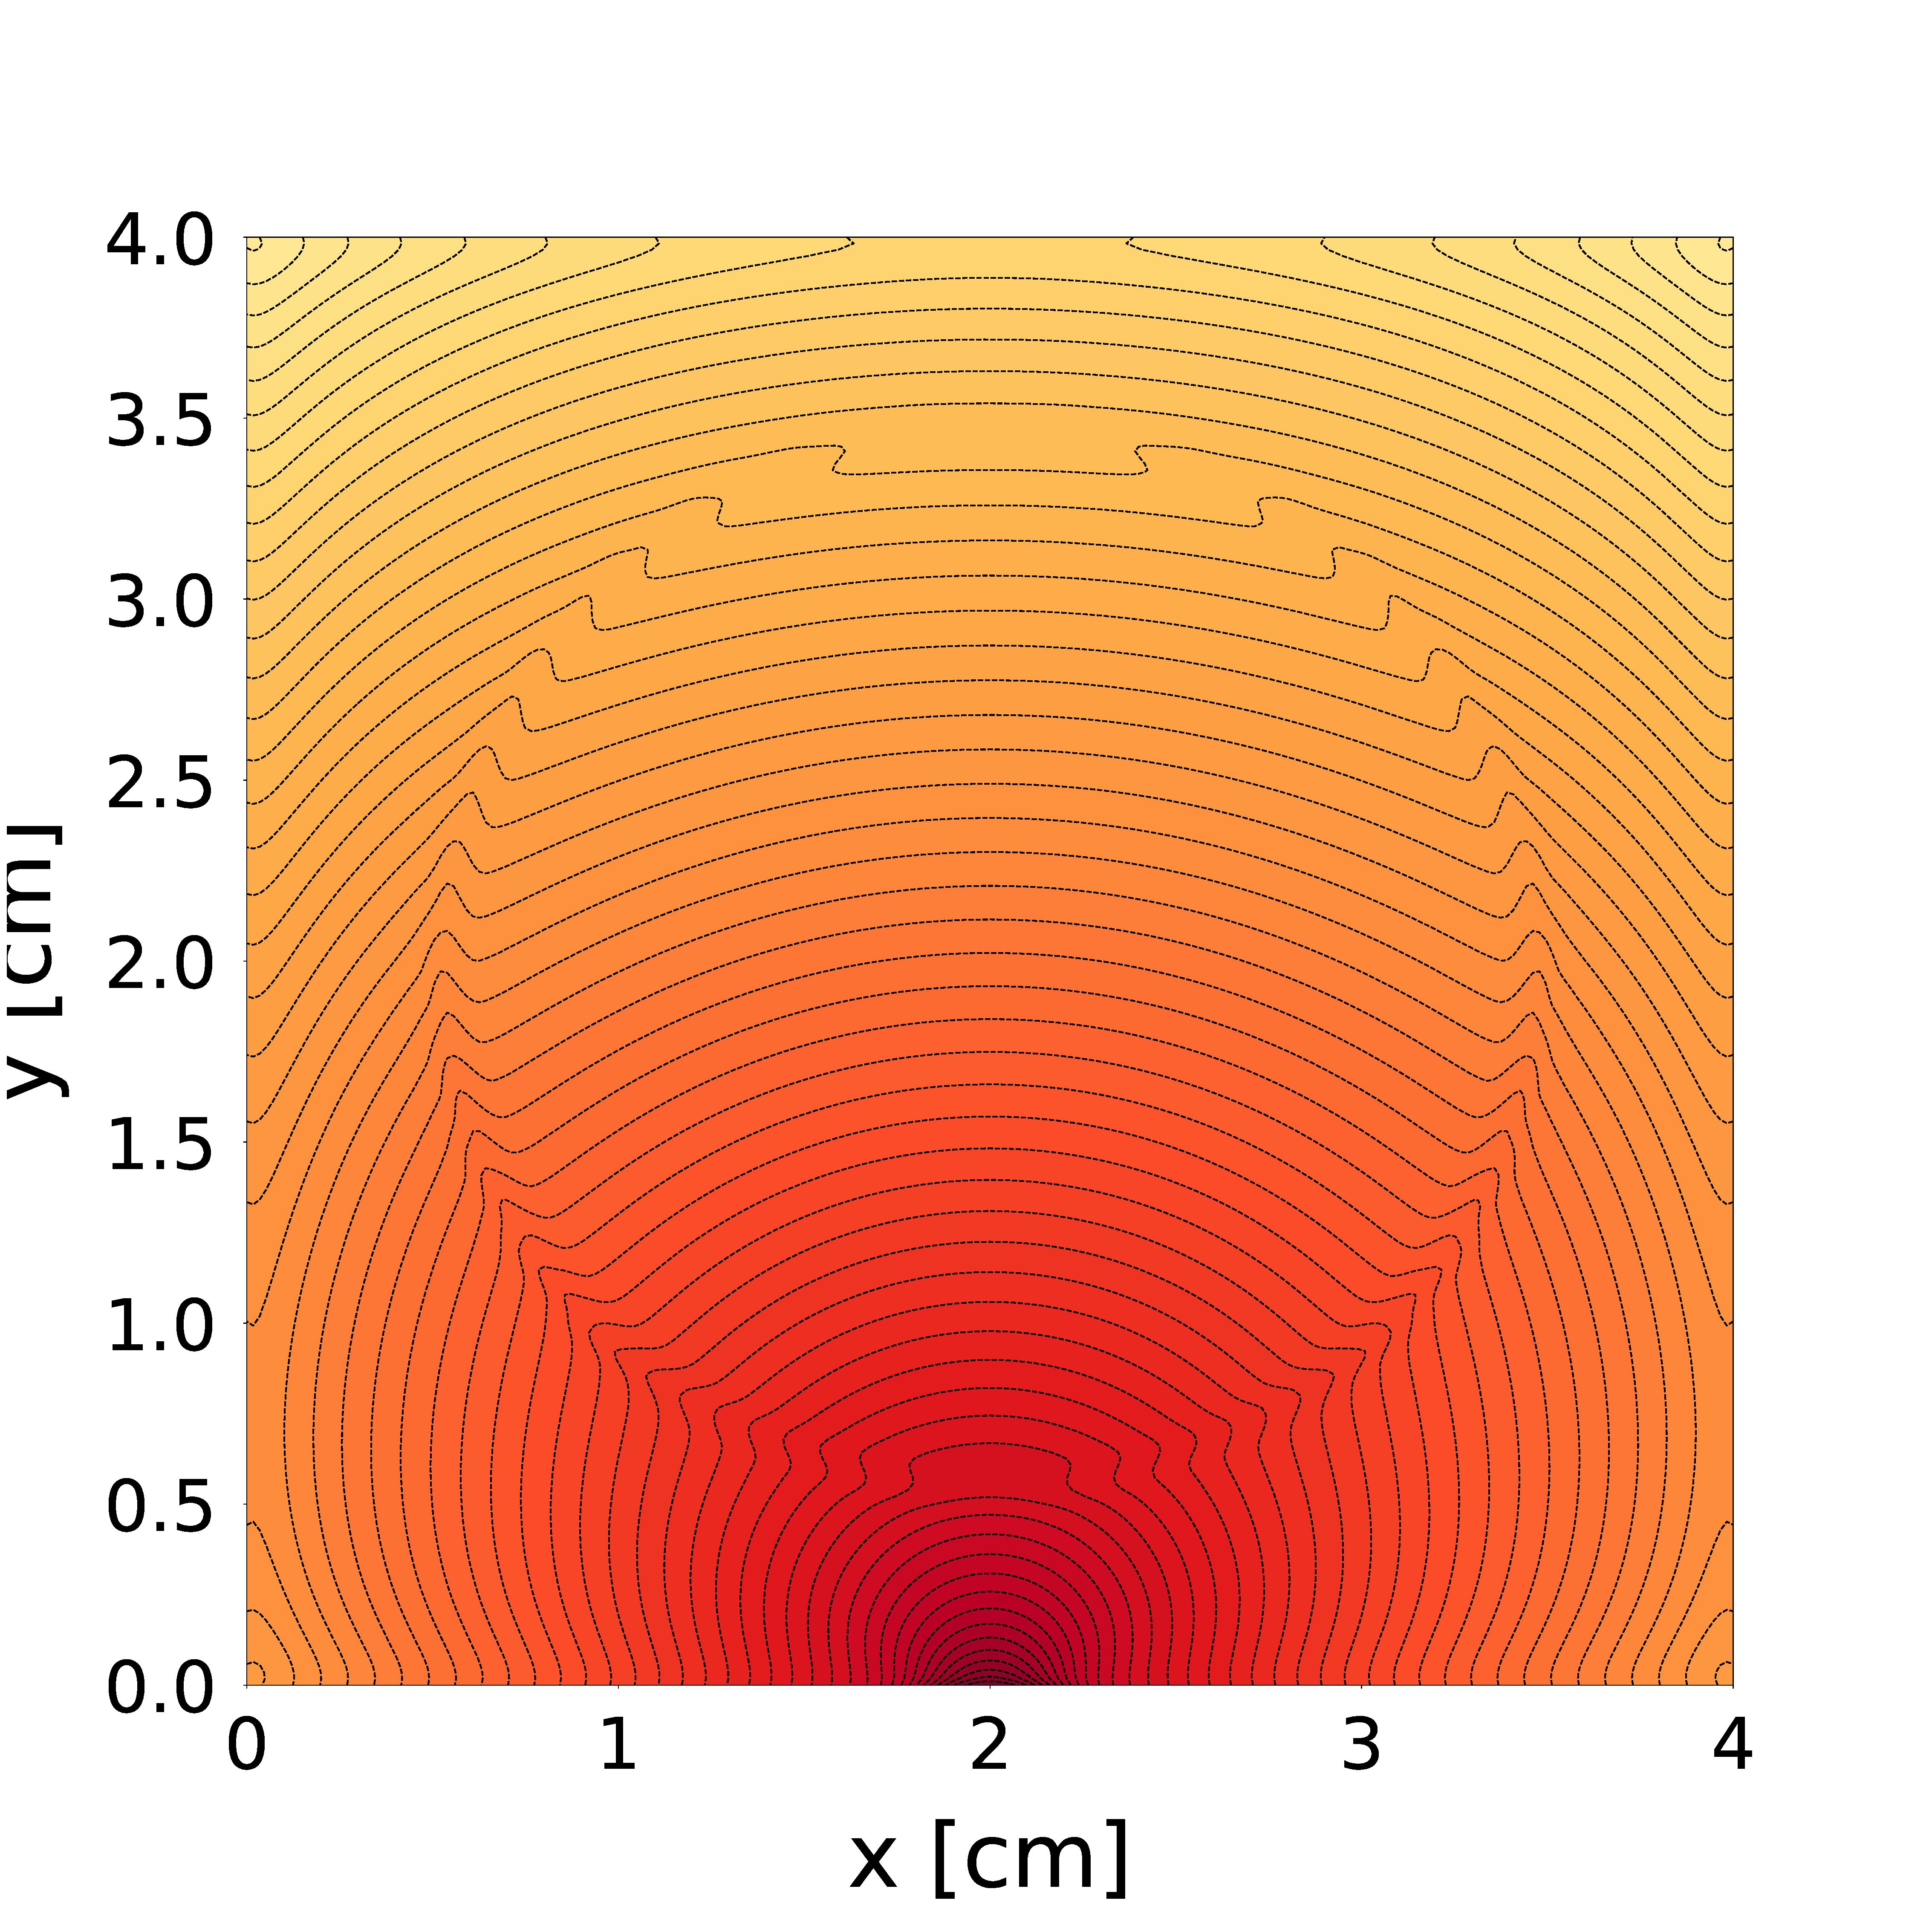
\includegraphics[width=0.32\linewidth]{figuras/ph2A.eps}
  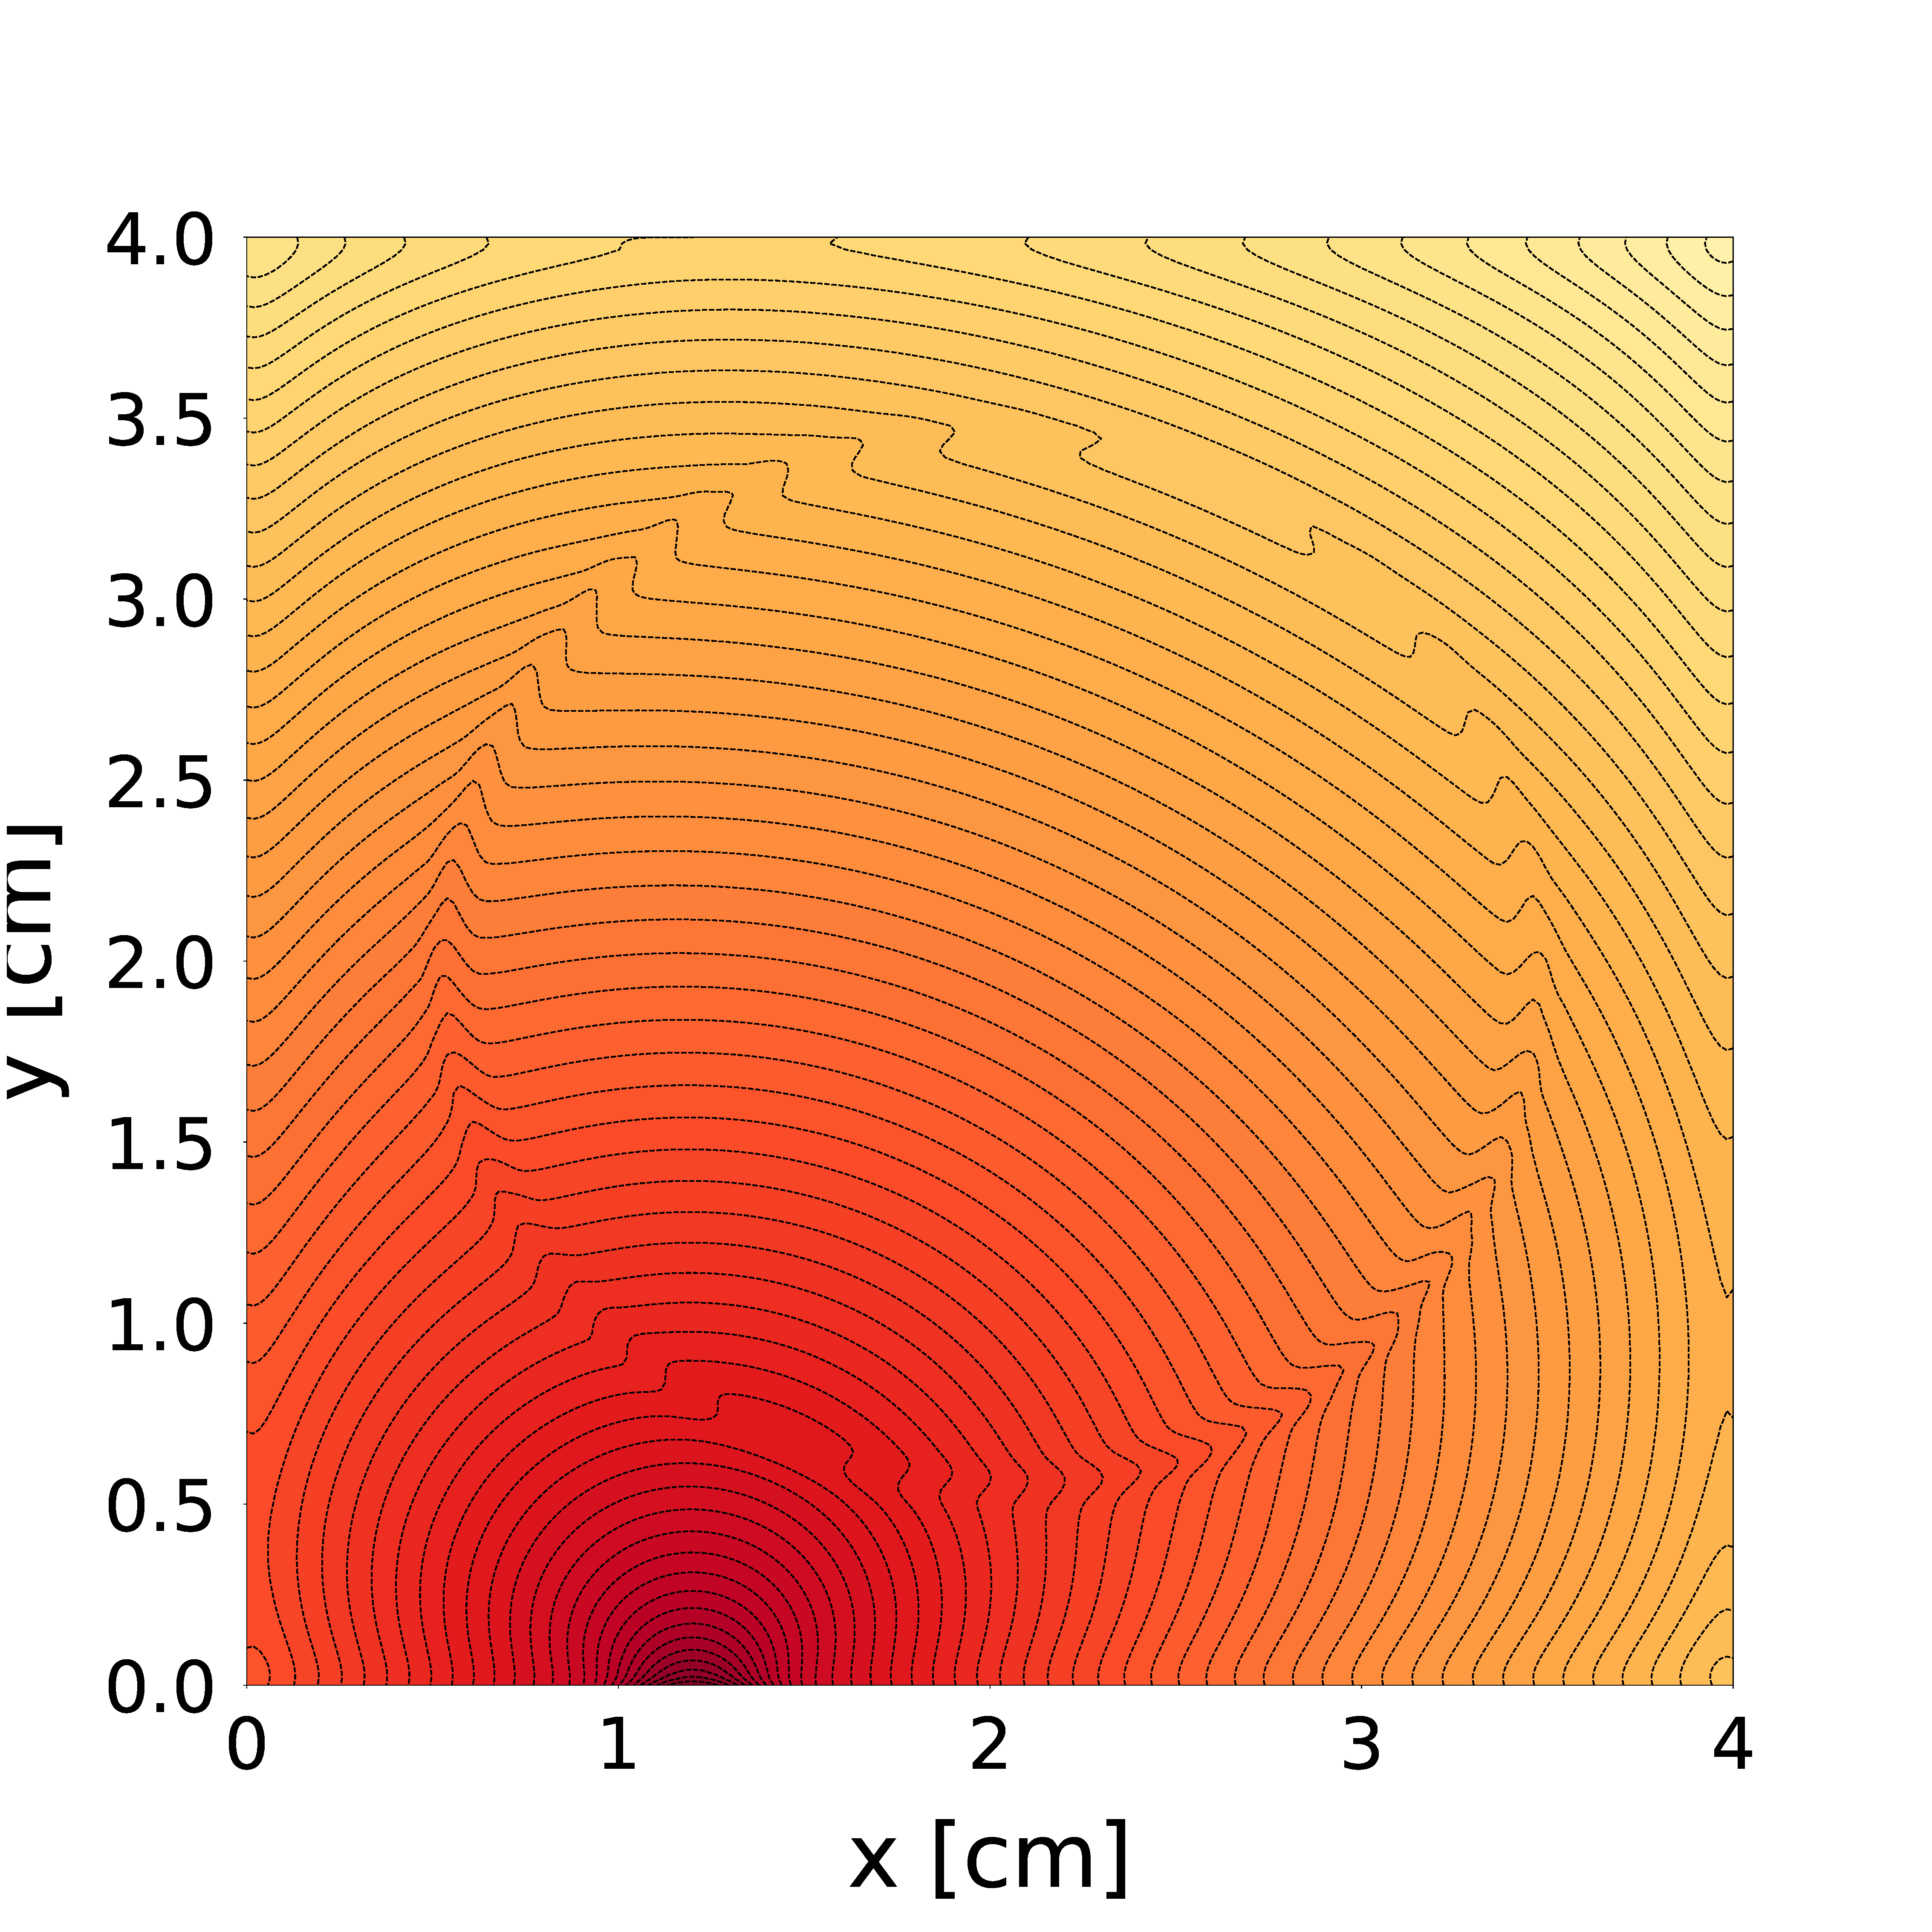
\includegraphics[width=0.32\linewidth]{figuras/ph2B.eps}
  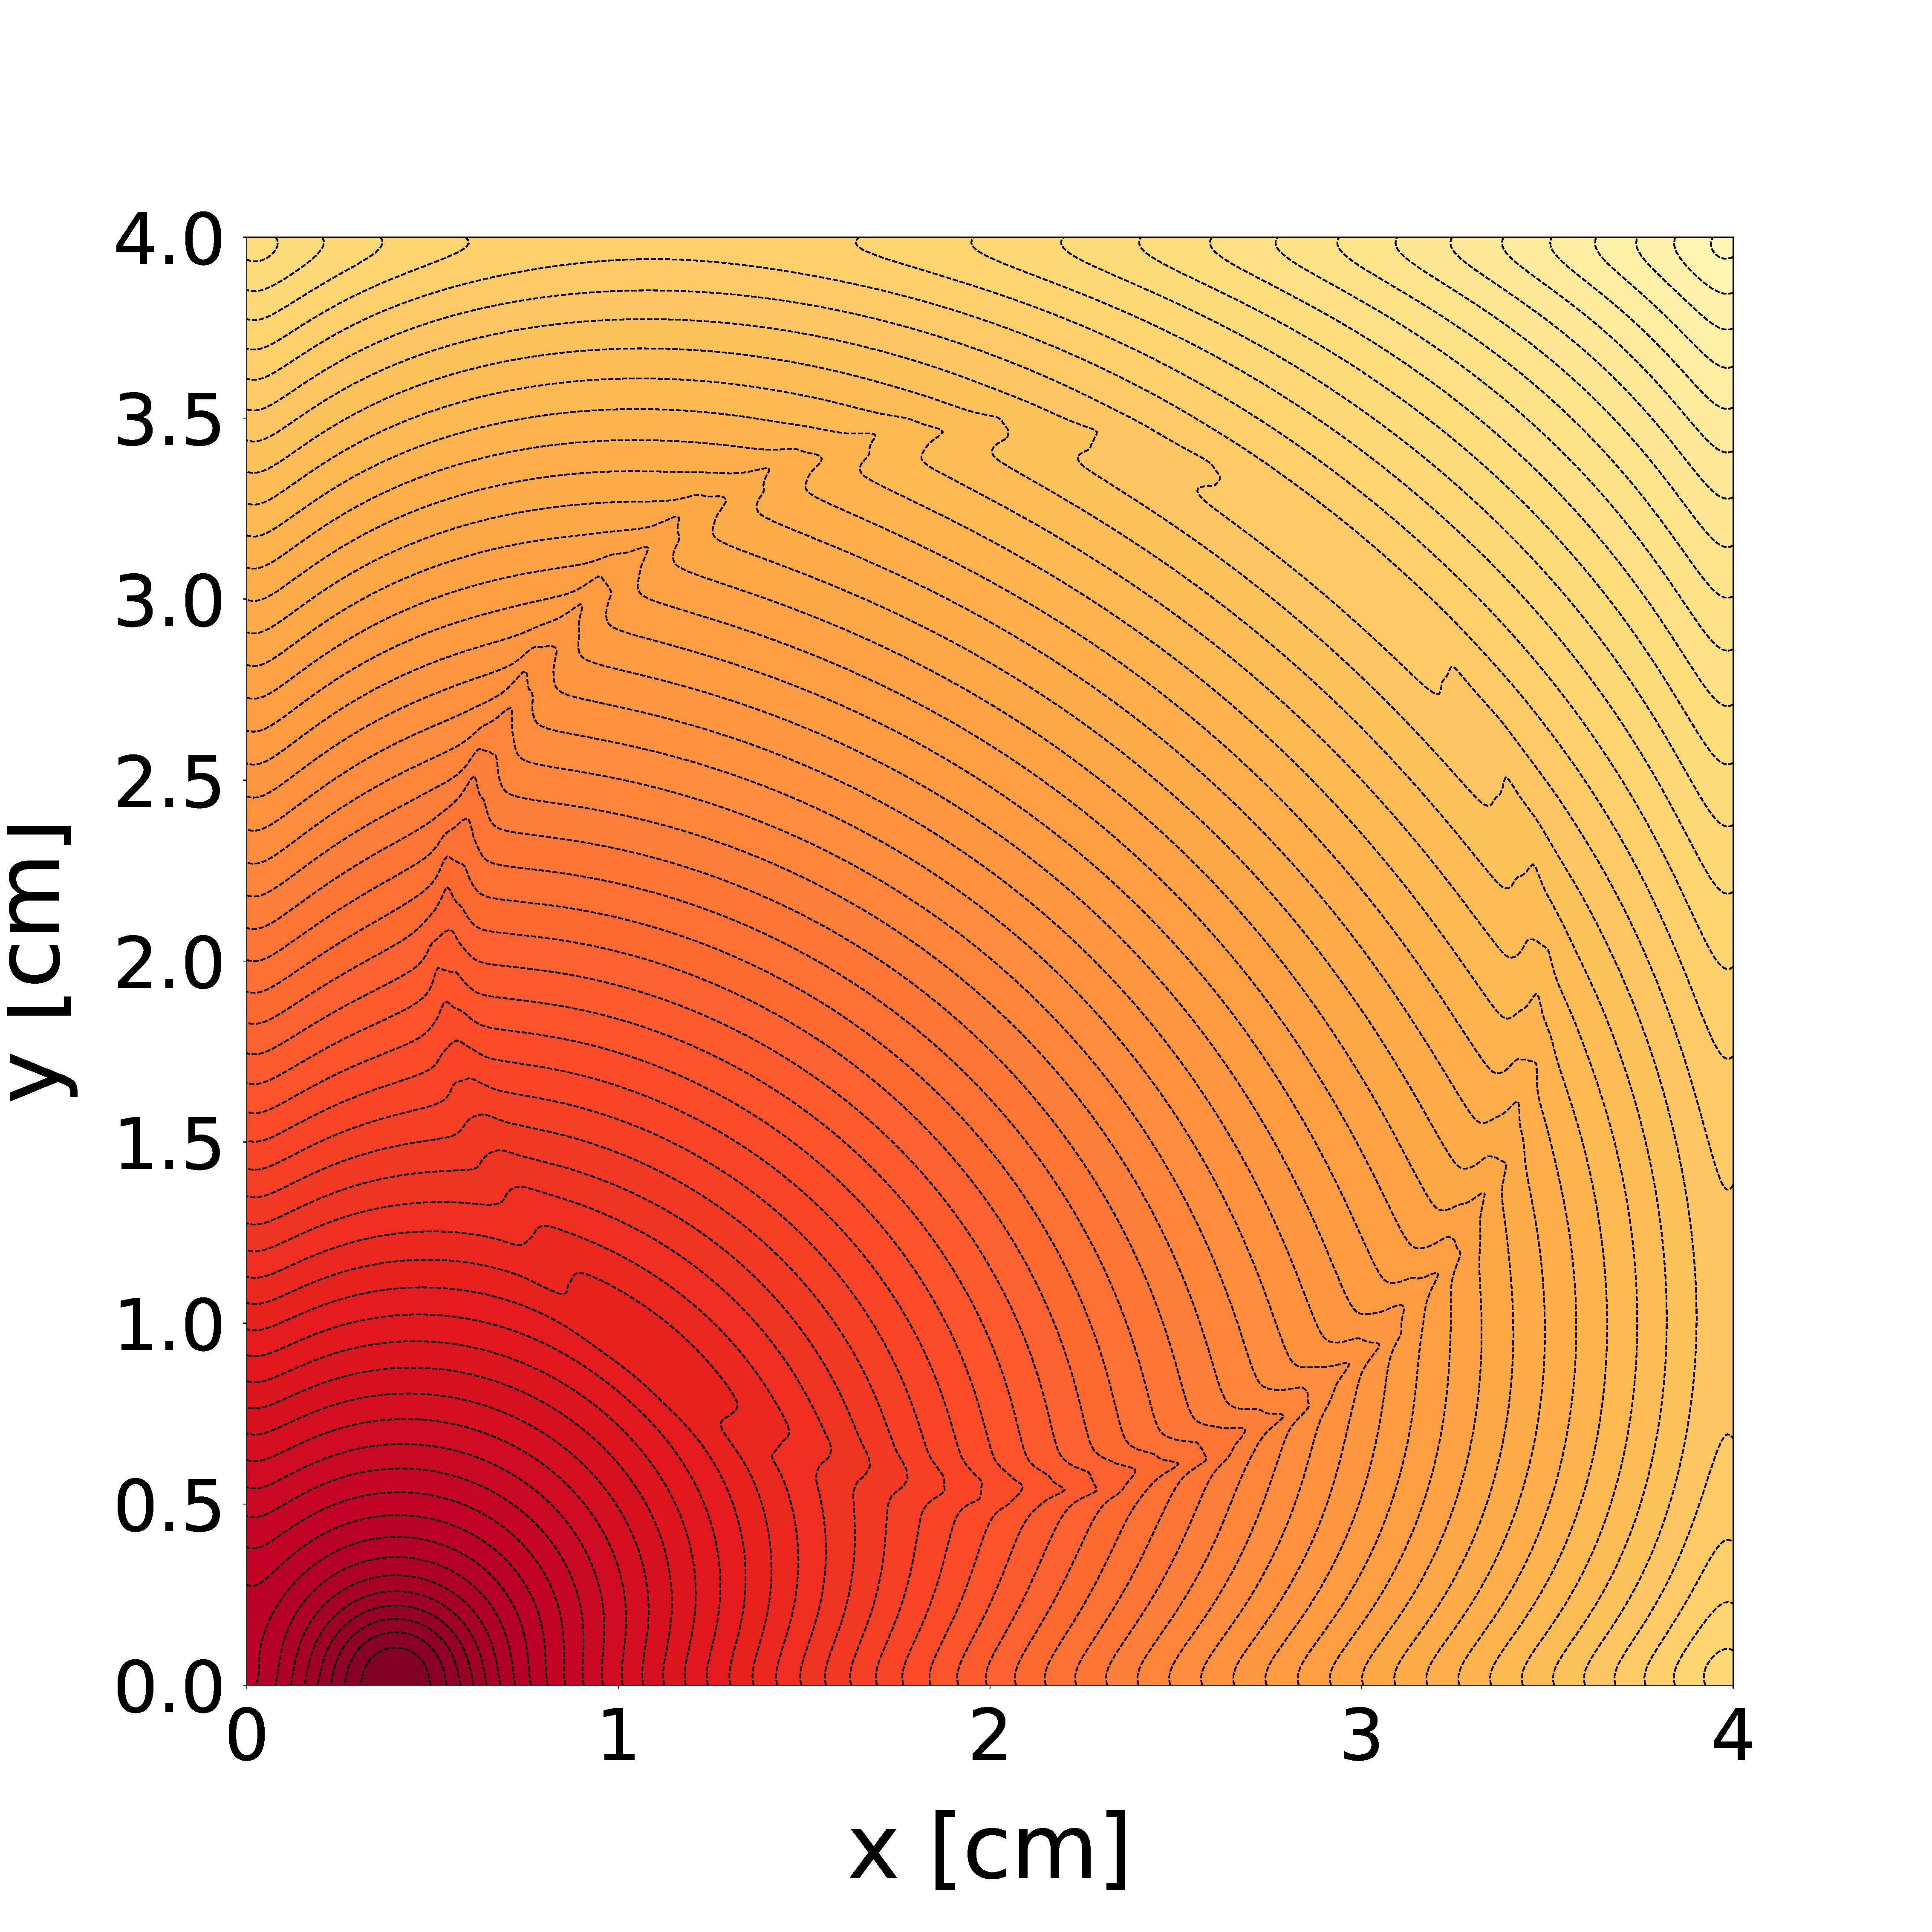
\includegraphics[width=0.32\linewidth]{figuras/ph2C.eps}
  \caption{Flujo escalar $\phi(\x)$~\eqref{eq:photondensity} 
  obtenido en las simulaciones para el fantoma inhomogéneo. A (izquierda), B (centro) y C (derecha).}
 \label{fig:ph2timef}
\end{figure}
Estos resultados muestran claramente el efecto de la región de vacío. 
En esta región, los fotones viajan libremente. Esta característica 
implica que este problema no puede ser correctamente resuelto 
mediante la aproximación de difusión.
El flujo de fotones que llegan a los 38 detectores ubicados en la frontera del 
dominio se muestra en la figura~(\ref{fig:fluxph2}). 
Se observa un buen acuerdo entre teoría y experimento, aunque 
con mayores desviaciones respecto al caso del fantoma homogéneo. 
Estas desviaciones pueden explicarse por el hecho de que 
en nuestras simulaciones no estamos teniendo en cuenta la reflexión 
de Fresnel que ocurre en la interface del anillo cilíndrico, 
lo cual requeriría de un tratamiento especial~\cite{Bal2006}. 

La presencia de regiones de vacío, como la que se encuentra en el 
fluido cerebroespinal en la cabeza, o entre órganos en el cuerpo 
--el fluido sinovial en las articulaciones~\cite{Netz2001}, 
o la traquea en el cuello humano~\cite{Fujii2016}--, 
requiere del uso de la ETR como modelo físico, ya que la 
aproximación de difusión de fotones no es apropiada en este régimen de transporte. 
\begin{figure}[h!]
\centering
  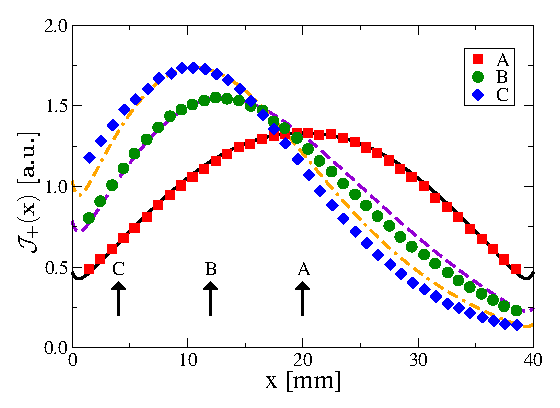
\includegraphics[width=0.48\linewidth]{figuras/kloseph2x.eps}
  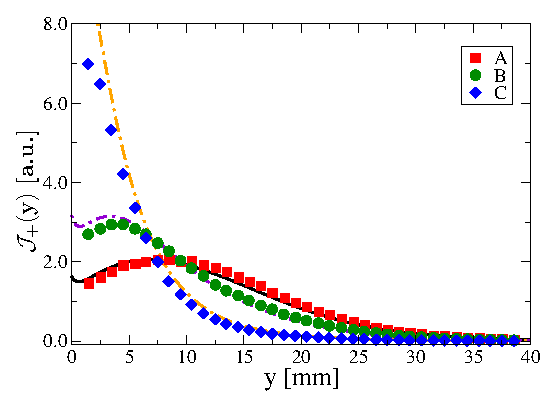
\includegraphics[width=0.48\linewidth]{figuras/ph2y.eps}
  \caption{Radiación transmitida medida por Klose~\cite{Klose2002} (símbolos),
  y radiación obtenida mediante las simulaciones FC--DOM, para 
  el fantoma inhomogéneo (líneas).}
 \label{fig:fluxph2}
\end{figure}
Tanto este experimento como el previo, han sido simulados por Klose {\it et al.} 
\cite{Klose2002} mediante el uso de diferencias finitas, utilizando la ETR 
independiente del tiempo.

\subsection{El fenómeno de rayos}
\label{subsec:rayeff}
En esta sección presentamos el último caso independiente del tiempo 
que trataremos en esta tesis. Este concierne a un 
fenómeno importante que surge en las aproximaciones numéricas 
que utilizan métodos de ordenadas discretas para resolver la ETR~\cite{Lewis1984}. 
Se trata del fenómeno de rayos, 
el cual se manifiesta esencialmente en medios de baja dispersión. 
El fenómeno de rayos se origina debido a la discretización 
de la variable angular $\hth$. Debido a dicha discretización, 
las direcciones posibles para la propagación de los fotones 
se encuentra limitada. Cuando existen fuentes localizadas, 
se originan variaciones rápidas en la intensidad específica 
cerca de estas. La propagación del flujo queda restringida 
en las direcciones discretas, dando origen a oscilaciones 
espurias, conocidas como efecto de rayos. 

Analizamos un problema  
de referencia ampliamente utilizado, 
diseñado específicamente para estudiar este efecto numérico.
Dadas las dimensiones del mismo, 
los fotones no llegarán a sufrir suficientes eventos de colisión.
Reproducimos 
el caso reportado por Crosbie y Schrenker~\cite{Crosbie1984}, 
el cual proporciona flujos considerados exactos~\cite{Ramankutty1997,tagnekamdem2015}, 
utilizando el método FC--DOM para soluciones independientes 
del tiempo obtenidas por relajación del caso dependiente del tiempo. 

Consideramos un dominio bidimensional cuadrado, de lado unitario, 
que contiene un medio puramente dispersivo (sin absorción) 
con $b(\x)=1$. La dispersión considerada es isótropa ($g=0$). 
La radiación incide de manera uniforme sobre la superficie inferior del medio. 
El resto de los bordes presentan condiciones de contorno de vacío ($n_{\Omega}=n_{s}$ 
de donde $f(\hth \cdot \hnu)=0$). El observable considerado es la componente en
 $y$ de la corriente de fotones~\eqref{eq:photoncurrent} $\mathcal{J}_y(x,y=1)$. En la Figura~(\ref{fig:fluxph3}) 
se presentan los resultados obtenidos (líneas), y los valores de referencia (símbolos). 
Se observa que el efecto de rayos se manifiesta en discretizaciones 
relativamente gruesas de la variable angular, y disminuye al aumentar 
el número de direcciones. 
El método de continuación de Fourier sólo trata 
al operador diferencial en las variables espaciales, independientemente 
de la discretización angular. Por lo tanto, no 
resuelve el fenómeno de rayos y otras estrategias deben ser consideradas 
para solucionarlo.
\begin{figure}[h!]
\centering
  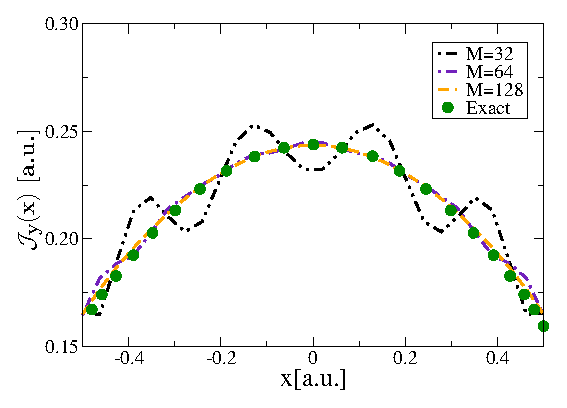
\includegraphics[width=0.48\linewidth]{figuras/raycurrent.eps}\\
  \caption{
Círculos: corriente de fotones exacta en la dirección $y$, $\mathcal{J}_y(x)$. 
Líneas: valores simulados obtenidos por el método FC--DOM, 
para un número variable de direcciones: $M=32,64,128$. El gráfico 
se presenta en unidades arbitrarias (a.u).}
 \label{fig:fluxph3}
\end{figure}

En medios altamente dispersivos, el comportamiento singular 
que origina el fenómeno de rayos resulta rápidamente atenuado lejos 
de la fuente, debido a que la radiación directa 
(los fotones balísticos que no han sufrido dispersión) decaen rápidamente
~\cite{Ramankutty1997}, redistribuyendo la radiación en todas las 
direcciones. Este fenómeno no suele ser un problema en tejidos biológicos, 
ya que estos son altamente dispersivos.

\subsection{Comparación con solución analítica}

En esta sección validamos nuestros métodos computacionales 
dependientes del tiempo calculando el flujo escalar, 
y comparándolo con la solución analítica dada por Paasschens~\cite{Paasschens1997} 
para una fuente puntual en un medio infinito. 
En el problema presentado por Paasschens, un medio bidimensional infinito, 
isótropo y homogéneo es iluminado por una fuente puntual isótropa
ubicada en el origen de coordenadas $s(\x,\hth,t)=\delta(\x)\delta(t)$.

La solución para este problema es
\begin{equation}
\begin{split}
\begin{aligned}
\phi(r,t)=\frac{e^{-c t \, (a+b')}}{2\pi}\delta(ct-r)&+\frac{b'}{2\pi c t}\left(1-\frac{r^2}{c^2t^2}\right)^{-1/2}\\
&\times\exp\left[b'\sqrt{c^2t^2-r^2}-c t \, (a+b')\right]H(ct-r),
\end{aligned}
\end{split}
\label{eq:Paasschenssc}
\end{equation}
donde $H(x)$ es la función escalón de Heaviside, 
y se ha hecho uso del coeficiente de dispersión reducido $b'=(1-g)b$, 
el cual aproxima la anisotropía en la dispersión manteniendo una 
función de fase isótropa.

Para este cálculo, simulamos un fantoma homogéneo con las propiedades ópticas 
dadas en la tabla~\ref{tab:tabopt}, de donde $c=0.019$cm/ps.

El primer término en la expresión~\eqref{eq:Paasschenssc} 
representa el pico balístico~\cite{Paasschens1997}, originado 
por los fotones que no han sufrido dispersión, y que arriban al punto 
a una distancia $r$ de la fuente en un tiempo $t=r/c$.

En el caso de medios altamente dispersivos, este término resulta rápidamente atenuado 
a unos pocos milímetros de la fuente. Para las simulaciones numéricas 
empleamos condiciones de borde de vacío, en las cuales el flujo 
entrando a través de la superficie del dominio $\partial \Omega$ es nulo 
\begin{equation}
u(\x,\hth,t)=0 \;\;\; \text{en}\; \Gamma_{-} \, .
\label{eq:vacuumbc}
\end{equation}
A los efectos prácticos, para evitar inestabilidades originadas 
por el fenómeno de Gibbs, y demandas computacionales significativas, 
la función delta de Dirac de la fuente es aproximada con una función Gaussiana.

Además, comparamos los resultados numéricos obtenidos por el método FC--DOM (FC)
con una aproximación al gradiente espacial obtenido por el método ''upwind´´ 
de diferencias finitas de tercer orden (FD) utilizado en \cite{Fujii2014}. 
En la figura~ \ref{fig:analytic1} se muestran los resultados obtenidos por ambos métodos 
junto con la solución analítica. En ambos casos el acuerdo es excelente.

 \begin{figure}[h]
\centering
  \includegraphics[width=0.48\linewidth]{figuras/analytic1.eps}
  \caption{Solución analítica ec.~\eqref{eq:Paasschenssc}, 
  y soluciones numéricas obtenidas por el método FC--DOM (FC) 
  y FD--DOM (FD) para un medio homogéneo ``infinito'' iluminado 
  por un pulso puntual.}
 \label{fig:analytic1}
\end{figure}
 
Para dar una idea cuantitativa de la convergencia obtenida para el método 
FC en comparación con el método de diferencias finitas empleado, 
definimos el error con respecto a la solución analítica cómo
\begin{equation}
\Delta \phi(r)= 
\sqrt{
\frac{ \int_{t_0}^{t_f} |\phi^a(r,t)-\phi^n(r,t)|^2 \,  dt}
{\int_{t_0}^{t_f} \phi^a(r,t)^2 \, dt } 
} \, , 
\end{equation}
donde $\phi^a(r,t)$ es el flujo escalar analítico~\eqref{eq:photondensity}, 
y $\phi^n(r,t)$ son los flujos escalares obtenidos a partir de las 
simulaciones numéricas, con los métodos FC y FD. 
Utilizamos un tiempo inicial $t_0=70$ps y un tiempo final 
$t_f=400$ps. El tiempo inicial es elegido de forma tal que el pico balístico 
ya paso el punto de observación $r$, evitando así el comportamiento 
singular del mismo. El tiempo final es elegido de forma tal 
de evitar efectos de borde. En contraste con el acuerdo 
cualitativo mostrado en la figura~\ref{fig:analytic1}, 
los errores furon calculados en este caso sin normalización, 
y en lugar de utilizar la función Gaussiana como aproximación, 
la solución analítica (ec.~(26) en la referencia~\cite{Paasschens1997}) 
a $t=t_0$ fue utilizada como condición inicial para evolucionar temporalmente 
la solución hasta el tiempo final $t_f$. 
Este procedimiento da una aproximación exacta a la solución a $t=t_0$, 
evitando errores numéricos asociados al comportamiento singular de la función 
delta de Dirac. 
Consideramos el error $\Delta \phi (r,t)$, con $r=1.27$cm desde la fuente. 
En la tabla~\ref{tab:convFCanalytic} mostramos los errores producidos por los métodos FC y FD 
para una simulación utilizando $M=16$ direcciones discretas, con $T=3.3\times 10^5$ 
pasos temporales, y un número variable de puntos en las coordenadas espaciales, 
con $\Delta =\Delta x =\Delta y$.

\begin{table}[h!]
\caption{Convergencia con respecto al flujo escalar analítico} 
\vspace{-0.3cm}
\begin{center}
\begin{tabular}{ccccc}
\hline
  ~~$\Delta$~~  &  ~~$\Delta \phi_{FC}(r)$~~   &   ~~$\Delta \phi_{FD}(r)$ ~~ \\
\hline
 ~~0.250~~   &  ~~$5.8\times 10^{-3}$~~  &  ~~$1.5\times 10^{-1}$~~   \\
 ~~0.125~~   &  ~~$1.8\times 10^{-4}$~~  &  ~~$2.2\times 10^{-2}$~~   \\
 ~~0.100~~   &  ~~$4.7\times 10^{-5}$~~  &  ~~$1.1\times 10^{-2}$~~    \\
\hline
\end{tabular}
\label{tab:convFCanalytic}
\end{center}
\end{table}
La tabla~\ref{tab:convFCanalytic} muestra claramente que el error obtenido 
del uso del método FC es significativamente menor al obtenido mediante el método FD, 
en órdenes de magnitud, y para todos los valores de $N$ probados. 
Esto puede explicarse en el hecho de que el método FC, a diferencia de 
los métodos de diferencias finitas y elementos finitos, es un método que 
por ser espectral, presenta un error de dispersión despreciable.

\section{Existencia de capa límite}
\label{sec:blayer}
En secciones previas demostramos el alto órden de convergencia numérica 
del método FC--DOM propuesto para el caso de soluciones manufacturadas.

La solución manufacturada que utilizamos en la sección~\ref{sec:manufacturada}
es suave, y no presenta gradientes significativos en ninguna de sus variables. 
Los teoremas de convergencia para los métodos numéricos exigen, en general,  
ciertas condiciones de regularidad de las soluciones subyacentes que se intentan aproximar. Cuando las soluciones, 
o sus derivadas, no son continuas, los métodos no presentaran el órden 
de convergencia deseado. El orden de convergencia de los métodos numéricos 
depende, en general, de la regularidad de la solución y sus derivadas. En particular, en esta sección estudiaremos 
una estructura de capa límite~\cite{Gaggioli2021} que existe de forma casi ubicua en las soluciones 
a la ecuación ETR, que no había sido previamente detallada en la bibliografía, 
y que representa una dificultad para la solución numérica de la ETR con alta precisión.
En esta sección nos valdremos de la versión en una única dimensión espacial de la ETR, 
para el caso independiente del tiempo. 
Esto se corresponde a problemas de tres dimensiones con simetría de traslación en dos 
de las variables espaciales. El modelo en una dimensión independiente del tiempo representa el caso 
más simple para el estudio de la capa límite, y análisis que realizaremos
se aplica a los casos multidimensionales en el dominio temporal. 

El contexto de esta sección será ligeramente diferente al de secciones previas, 
ya que abundará en referencias bibliográficas en el contexto 
del análisis de transporte de neutrones. La razón de ello 
es que en el análisis realizado de la bibliografía, encontramos 
que las escasas menciones que se hacen a esta estructura de capa límite, 
que a nuestro criterio no había sido correctamente descripta ni detallada, 
son en el contexto de transporte de neutrones. Esta estructura 
de capa límite ayuda a explicar problemas numéricos reportados en la bibliografía 
a lo largo de décadas
(en particular, las oscilaciones que ocurren en la llamada 
``discretización de diamante''), fenómeno numérico el cual, a nuestro 
criterio, no había sido correctamente comprendido hasta ahora.

Si bien el desarrollo de métodos numéricos de alto órden de 
convergencia para la ecuación de transporte en problemas más 
generales de varias dimensiones para los casos más generales 
escapa al alcance de esta tesis, nuestro trabajo 
sienta los cimientos para el desarrollo de métodos numéricos 
altamente eficiente, como lo demostraremos para el caso 
de una dimensión espacial en el dominio temporal. El desarrollo 
de métodos numéricos eficientes de las mismas características para los casos 
multidimensionales requiere de métodos sofisticados como 
los elaborados en el contexto de las ecuaciones de Navier-Stokes~\cite{Bruno2019}, 
ya que requieren de métodos de evolución temporal implícitos, por las limitaciones 
que impone la condición de Courant–Friedrichs–Lewy al resolver con grillas apropiadas 
estas capa límite de naturaleza exponencial. Debido a la multidimensionalidad 
de la ETR, la implementación de métodos de evolución temporal implícitos 
pueden resultar sumamente costosos, y se requiere de estrategias 
sumamente eficientes para su implementación. Por este motivo, 
en esta sección nos límitamos al caso 1D, teniendo en cuenta que el mismo 
análisis aplica al caso multidimensional. 


Como se mencionó anteriormente, la ETR es una ecuación de Boltzmann linearizada, 
la cual provee de un modelo general para el transporte de partículas neutras, 
que no se limita al transporte de fotones, si no que incluye el caso de 
transporte de neutrones, la cual es utilizada en el modelado 
para el diseño y desarrollo de reactores nucleares entre otras disciplinas 
\cite{Chandrasekhar1960,Case1967,Lewis1984,Petrovic1996,Hunter2015,Barichello2016,Hu2020}.  
En esta sección identificamos y caracterizamos a una capa límite 
que, a pesar de presentarse \textit{e.g.}~en sistemas de autofunciones 
en problemas unidimensionales de transporte~\cite[Cap. 4]{Case1967}, 
no ha sido correctamente descripta previamente en la literatura. 
Los problemas numéricos que surgen al intentar resolver 
numéricamente la ETR son materia de una basta investigación 
y discusión en la literatura~\cite{Case1967,Lewis1984,Petrovic1996,Bal2001,Hunter2015} 
que se mantiene vigente. 

Esta estructura de capa límite presenta transiciones abruptas 
en las soluciones a la ETR, con gradientes de carácter exponencial 
que se dan en regiones cercanas a los bordes, para las direcciones 
entrantes que se aproximan a la dirección paralela al borde. 
Físicamente, esto se origina debido a que para dichas direcciones, 
las partículas atraviesan caminos geométricos relativamente grandes 
hacia el interior del dominio, lo que puede originar tanto decaímientos 
como crecimientos exponenciales en la intensidad específica en dichas direcciones, 
dependiendo de la naturaleza del problema.
\begin{figure}[h!]
\centering
  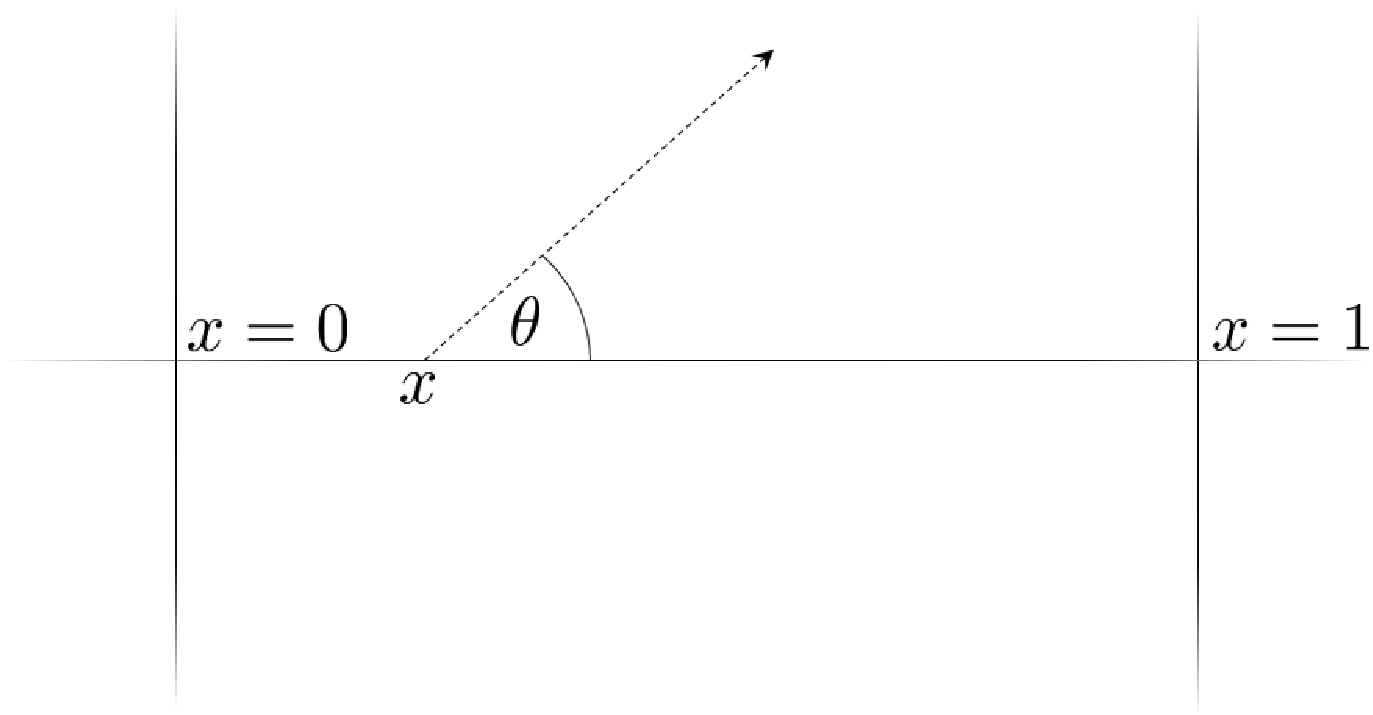
\includegraphics[width=0.5\linewidth]{figuras/geom.pdf}
  \caption{Geometría unidimensional: $\xi = \cos(\theta)$.}
 \label{fig:parallelgeom}
\end{figure}
La ecuación ETR independiente del tiempo, en una dimensión espacial 
modela el transporte en una geometría plano paralela descripta en la 
figura~\ref{fig:parallelgeom}. Por simplicidad, consideramos 
el caso isótropo, con condiciones de borde de Fresnel
\begin{equation}
\begin{split}
  &\xi \frac{\partial}{\partial x}\uxi+\mu_t(x)\uxi=   \frac{\mu_s(x)}{2} \int_{-1}^{1}\uxp d\xi' +q(x,\xi),\\
  &u(x=0,\xi)=\mathcal{R}(\xi)u(x=0,\xi_R) \; \forall \xi>0,\\
  &u(x=1,\xi)=\mathcal{R}(\xi)u(x=1,\xi_R) \; \forall \xi<0.
\end{split}
\label{eq:transp1d}
\end{equation}
donde $\xi=\cos(\theta)$,  $\mu_s(x)$ y $\mu_a(x)$ denotan 
los coeficientes de dispersión y absorción respectivamente, 
llamamos $\st(x)=\sa(x)+\mu_s(x)$ al coeficiente de transporte 
total, y $q(x,\xi)$ representa una fuente externa. Las condiciones de 
borde de Fresnel modelan la reflexión de las partículas en el borde, 
donde $\xi_R=-\xi$ representa el coseno de la dirección reflejada 
y $\mathcal{R}(\xi)$ es el coeficiente de Fresnel correspondiente~\cite{Born1999}.

Dado que el coeficiente $\xi$ que acompaña a la derivada de mayor 
orden en~\eqref{eq:transp1d} tiende a cero cuando $\theta \to \pi/2$, 
se espera que ocurra una capa límite que presente variaciones rápidas 
en la solución $u(x,\xi)$ para tales direcciones, y para valores 
de $x$ en regiones cercanas a los bordes en $x=0$ y $x=1$~\cite[Cap. 9]{Bender1999}, 
teniendo como consecuencia la existencia de gradientes que 
tienden a infinito para puntos $(x,\xi)$ cercanos a $(0,0)$ y $(1,0)$. 
Estas estructuras de ``capa límite'', que son generadas por 
la imposición de las condiciones de borde en conjunto con la existencia 
de un parámetro $\xi$ infinitesimal que acompaña a la derivada de mayor 
orden del operador diferencial, solo ocurren para las direcciones 
entrantes (salientes), con $\xi>0$ ($\xi<0$) para puntos cercanos 
a $x=0$, (resp. $x=1$)---dado que es para dichas direcciones que 
se imponen las condiciones de borde en la ecuación~\eqref{eq:transp1d}. 

Siguiendo la referencia~\cite{Bender1999}, para caracterizar
la estructura de capa límite en \eg $x=0$, utilizamos una 
{\em solución interna} de la forma $U(X,\xi) = u(\xi X,\xi)$; 
la capa límite alrededor de $x=1$ puede ser tratada de manera 
análoga. La solución asintótica de primer orden $U_0(X,\xi)$ 
de $U(X,\xi)$ cuando $\xi\to 0^+$ satisface la ecuación 
a {\em coeficientes constantes} 
\begin{equation}
\begin{split}
\frac{\partial U_0(X,\xi)}{\partial X}& + \mu_t(0) U_0(X,\xi)=\frac{\mu_s(0)}{2} 
\int_{-1}^{1} U_0\left(\frac{\xi X}{\xi'},\xi'\right) d\xi' +q(0,\xi),\\
\end{split}
\label{eq:transp1d2}
\end{equation}
con condiciones de borde inducidas por~\eqref{eq:transp1d}. 
La ecuación~\eqref{eq:transp1d2} nos dice que la derivada 
$\frac{\partial U_0(X,\xi)}{\partial X}$ se encuentra 
acotada cuando $\xi\to 0^+$, y, por lo tanto, que la función 
$U_0(X,\xi)$ caracteriza la estructura de capa límite 
en la solución $u(x,\xi)$ mediante la relación 
\begin{equation}
  u(x,\xi)\sim u_0(x,\xi) = U_0(x/\xi,\xi) \; \text{sí}  \;  (x,\xi)\to (0^+,0^+).
\end{equation}
El argumento puede extenderse a problemas en dos y tres dimensiones, 
incluyendo el dominio temporal y dominios generales curvos. En tales casos, 
la capa límite presenta gradientes que no están acotados 
en la proximidad de los bordes en direcciones paralelas a estos 
(situación que a escalas apropiadas se corresponde con la geometría 
de la fig.~\ref{fig:parallelgeom} para $\theta \to \pi/2$). 

Utilizando el factor integrante, y definiendo
\begin{equation*}
I(x,\xi) = \int_0^{x} e^{\frac{ \mu_t(0) y}{\xi}}\left[\frac{\mu_s(0)}{2} \int_{-1}^1u_0(y,\xi')d\xi'+q(0,\xi)\right]dy,
\end{equation*}
se obtiene
\begin{equation}
 u_0(x,\xi) = \frac{e^{-\mu_t(0)x/\xi}}{\xi} \Big[\xi u(0,\xi)+I(x,\xi)\Big] ,
 \label{eq:intf}
\end{equation}
la cual exhibe de manera explícita el carácter exponencial 
de la capa límite. Los diferentes términos de la solución asintótica 
para la capa límite poseen diferente significado físico. Expandiendo 
la igualdad~\eqref{eq:intf} podemos escribir:
\begin{equation}
\begin{aligned}
 u_0(x,\xi) =   e^{-\mu_t(0)x/\xi}\times u(0,\xi) + \frac{e^{-\mu_t(0)x/\xi}}{\xi} \times  \int_0^{x} e^{\frac{ \mu_t(0) y}{\xi}} \frac{\mu_s(0)}{2} \int_{-1}^1u_0(y,\xi')d\xi'dy&\\
 + \frac{e^{-\mu_t(0)x/\xi}}{\xi} \times \int_0^{x} e^{\frac{ \mu_t(0) y}{\xi}}  q(0,\xi) dy&,
 \label{eq:intfexpandida}
\end{aligned}
\end{equation}
donde el primer término representa el flujo entrante a través del borde en la dirección $\xi$ 
que no ha sufrido colisiones, el cual posee una atenuación exponencial 
debido a las interacciones de absorción y dispersión con el medio. El segundo término representa las contribuciones 
del medio debido a los procesos dispersivos, que sufren tanto una atenuación 
como un crecimiento exponencial, debido a la suma de contribuciones en el interior del medio. Finalmente, el último representa 
las contribuciones del medio debido a las fuentes $q$ en el interior de éste, 
las cuales también vienen dadas por contribuciones y atenuaciones en el interior del medio.

La estructura de capa límite puede visualizarse fácilmente 
considerando la solución exacta de la ecuación~\eqref{eq:transp1d} 
para el caso de coeficientes constantes sin dispersión ($\mu_s(x)=0$), 
de donde obtiene la solución analítica 
\begin{equation}
\begin{split}
u(x,\xi)=\begin{cases}
\displaystyle \frac{q}{\mu_a}\left[1-\frac{\eta(\xi)}{ e^{\mu_a x / \xi}}\right]&\forall\xi>0,\\[8pt]
%\displaystyle  \frac{q}{\mu_a}&\;\;\xi=0,\\
\displaystyle  \frac{q}{\mu_a}\left[1- \frac{\eta(\xi)}{e^{\mu_a (x-1) / \xi}} \right]&\forall\xi<0,
\end{cases}
\end{split}
\label{eq:transpnscatt}
\end{equation}
con
\begin{equation*}
\;\;\eta(\xi)=\frac{\mathcal{R}(|\xi|)-1}{\mathcal{R}(|\xi|)e^{-\mu_a/|\xi|}-1}.\qquad\qquad\qquad
\end{equation*}
Por simplicidad, consideramos condiciones de borde de vacío ($\mathcal{R}(\xi)=0$), 
la solución se muestra en la figura~\ref{fig:ansol}, donde se observa claramente la estructura de capa 
límite cuando $(x,\xi) \to (0^+,0^+)$.
\begin{figure}[h!]
\centering
  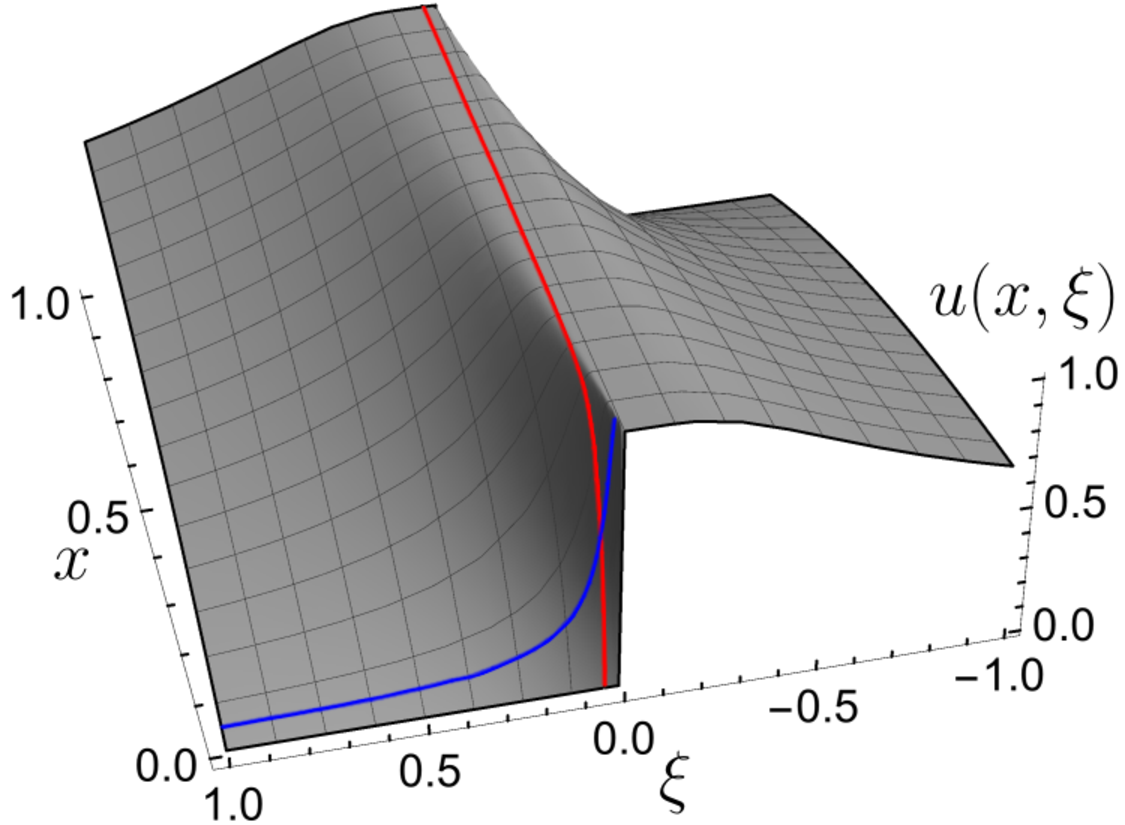
\includegraphics[width=0.5\linewidth]{figuras/Analytic_lay_3.pdf}
  \caption{Solución~\eqref{eq:transpnscatt} $\uxi$ de la ecuación.~\eqref{eq:transp1d} con
  $\mathcal{R}(\xi)=0$. Se observa la capa límite en las variables $x$ y $\xi$ 
  para $(x,\xi) \to (0^+,0^+)$ (enfatizadas en las curvas roja y azul).}
 \label{fig:ansol}
\end{figure}

Los dos métodos numéricos utilizados de manera predominante en la literatura 
para resolver la ecuación de transporte son 
el método de armónicos esféricos,  
y el método de ordenadas discretas. Ambos métodos fallan 
en la resolución de las estructuras de capa límite, 
lo cual puede apreciarse en resultados presentados 
en la literatura~\cite{Rocheleau2020,Wang2019,Harel2020,Anli2006,Chai1993}

En vista de la expresión~\cite[p. 77]{Trefethen2008} 
para el término del error en la cuadratura de integración 
de Gauss--Legandre, ampliamente utilizada en la literatura 
de ordenadas discretas, el error para la cuadratura de $\ell$-puntos 
decrece como $32V/15\pi j (2\ell+1-j)^j$ siempre que la derivada 
$j \leq 2\ell$ esté acotada por la constante $V$. 
Introduciendo el cambio de variable  $\xi'=r^p$ en la integral 
de la ecuación~\eqref{eq:transp1d}, buscamos una cota $V$ 
para la derivada $j$--ésima del integrando. 
Utilizando la versión integrada de la ecuación~\eqref{eq:transp1d}, 
similar a~\eqref{eq:intf}, combinando dos términos exponenciales, 
y utilizando el hecho de que para un entero no negativo $k$ 
la integral $\int_0^\infty t^k e^{-t} dt$ es finita, 
encontramos qué (apéndice~\ref{ap:demcv})
\begin{equation*}
\begin{split}
\left | \frac{\partial^j }{\partial r^j}\left[ u(x,r^p) r^{p-1}\right]
\right|\leq W r^{p-j-1}\; \text{para}  \; (x,r) \to (0^+,0^+),
\end{split}
\label{eq:boundedder}
\end{equation*}
para alguna constante $W$; llamando $V = W r^{p-j-1}$  
se obtiene la cota deseada, la cual es {\em uniforme 
para todos los valores relevantes de $x$ y $r$ } (siempre qué 
$p \ge j+1$). Los 
detalles de la demostración pueden encontrarse en el apéndice~\ref{ap:demcv}.

Para el caso considerado, con $\mathcal{R}(\xi)=0$, 
dividiendo la integral en el punto de capa límite $\xi=0$ se tiene 
\begin{equation}
\int_{0}^{1} u(x,\xi) d\xi \sim \sum_{i=1}^{M/2} w_i u(x,\xi_i),
\label{eq:MartensenKussmaul}
\end{equation}
donde, llamando $r_i$ y $w_i^{GL}$ a las abscisas y pesos de la 
cuadratura de Gauss--Legendre en el intervalo $[0,1]$, 
definimos $\xi_i=r_i^p$ y $w_i= p \times r_i^{p-1} \times w_i^{GL}/2$. 
Las abscisas y los pesos correspondientes a los valores negativos 
de $\xi$ se obtienen por simetría. 
\begin{figure}[h!]
\centering
  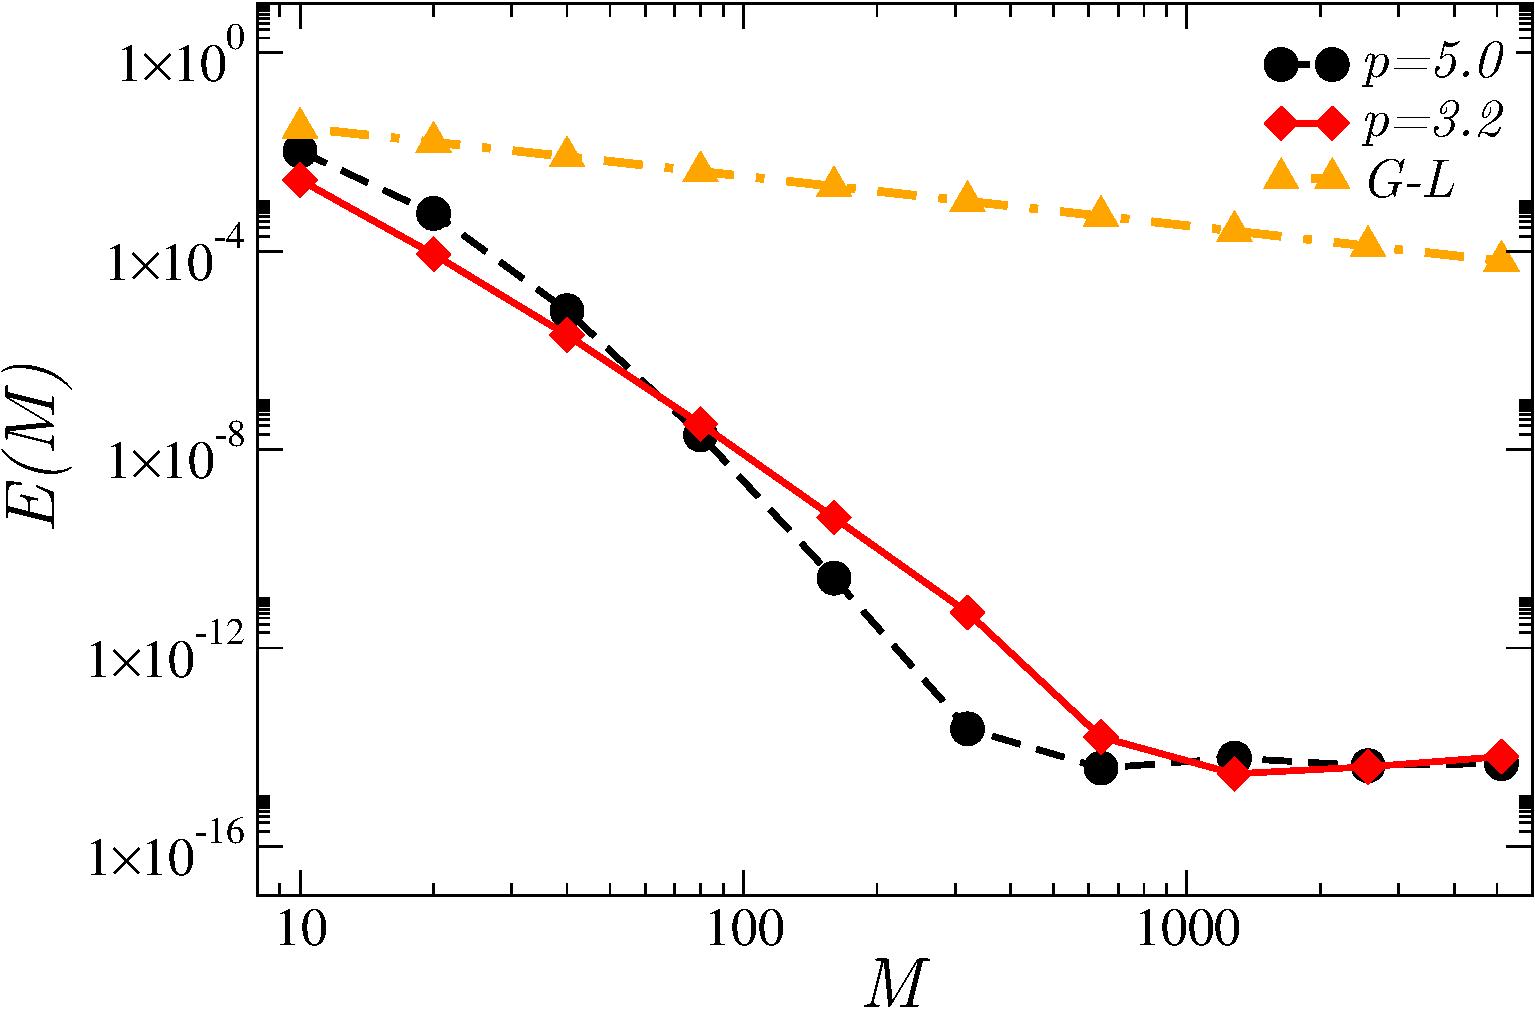
\includegraphics[width=0.5\linewidth]{figuras/quads.pdf}
  \caption{Error de la integral numérica comparado con la integral 
  analítica $E(M)=\text{max}_x |\sum_{i=1}^M w_i u(x,\xi_i)-I^{\text{an}}(x)|$
  obtenida para la solución dada en~\eqref{eq:transpnscatt} con $\mathcal{R}(\xi)=0$. 
  Los errores son comparados con los obtenidos para la cuadratura 
  de la ecuación~\eqref{eq:MartensenKussmaul}, donde 
  también se muestra el error dado por la cuadratura de  Gauss--Legendre
    (G--L) sin el cambio de variable típicamente utilizada.}
 \label{fig:intconvs}
\end{figure}
Se encontró el valor $p=3.2$ como óptimo, el cual 
provee una convergencia excelente para la integral 
de dispersión en la variable $\xi$, el cual a su vez limita la rapidez 
de las variaciones de la capa límite en la variable $x$. 
Para resolver la capa límite en la variable $x$, utilizamos 
el cambio de variable logarítmico $v=\log(\frac{x}{1-x})$, 
el cual origina una grilla de discretización espacial con una 
densidad de puntos exponencial en la cercanía de los bordes, 
con puntos extremadamente cercanos al borde (sin detrimento 
en la convergencia de la cuadratura de la integral colisional, 
en vista de las cotas halladas en la derivada del 
integrando con respecto a la nueva variable $r$ mencionada 
anteriormente, las cuales son {\em uniformes para todo $x$}), 
lo cual provee alto orden de convergencia en ambas variables $\xi$ y $x$

Resolvemos la ecuación de transporte que resulta en el nuevo dominio computacional
$[v_{\text{min}},v_{\text{max}}]$, con 
$[x'_{\text{min}},x'_{\text{max}}]=[\frac{e^{v_{\text{min}}}}{e^{v_{\text{min}}}+1},
\frac{e^{v_{\text{max}}}}{e^{v_{\text{max}}}+1}]$, 
y condiciones de bordes en $x'_{\text{min}}$ y $x'_{\text{max}}$ 
obtenidas a partir de la solución asintótica para la capa límite 
de la ecuación~\eqref{eq:intf}. Utilizando las nuevas variables, 
resulta el problema de transporte dependiente del tiempo
\begin{equation}
\begin{split}
&\frac{\partial}{\partial t}\uvi+\xi(2+2\cosh(v)) \frac{\partial}{\partial v}\uvi+
\st\uvi=\sct \int_{-1}^{1} \uvp d\xi'+q, \\
&u(v,\xi,t_{\text{min}})=0,\\
&u(v_{\text{min}},\xi,t)=u_{0}(x'_{\text{min}},\xi,t) \; \forall \xi>0,\\
&u(v_{\text{max}},\xi,t)=u_{0}(x'_{\text{max}},\xi,t) \; \forall \xi<0.
\end{split}
\label{eq:transptd}
\end{equation}
Con el fin de evitar las
limitaciones impuestas por la condición de Courant–Friedrichs–Lewy, utilizamos un 
esquema implícito BDF (backward differentiation formula) de evolución temporal de tercer orden. 
Para evitar el alto costo en la inversión de matrices grandes a 
cada paso temporal, el término 
colisional se obtiene por extrapolación polinomial. La versión discreta 
de la ecuación~\eqref{eq:transptd} resulta\looseness=-1
\begin{wrapfigure}{r}{0.45\textwidth}
  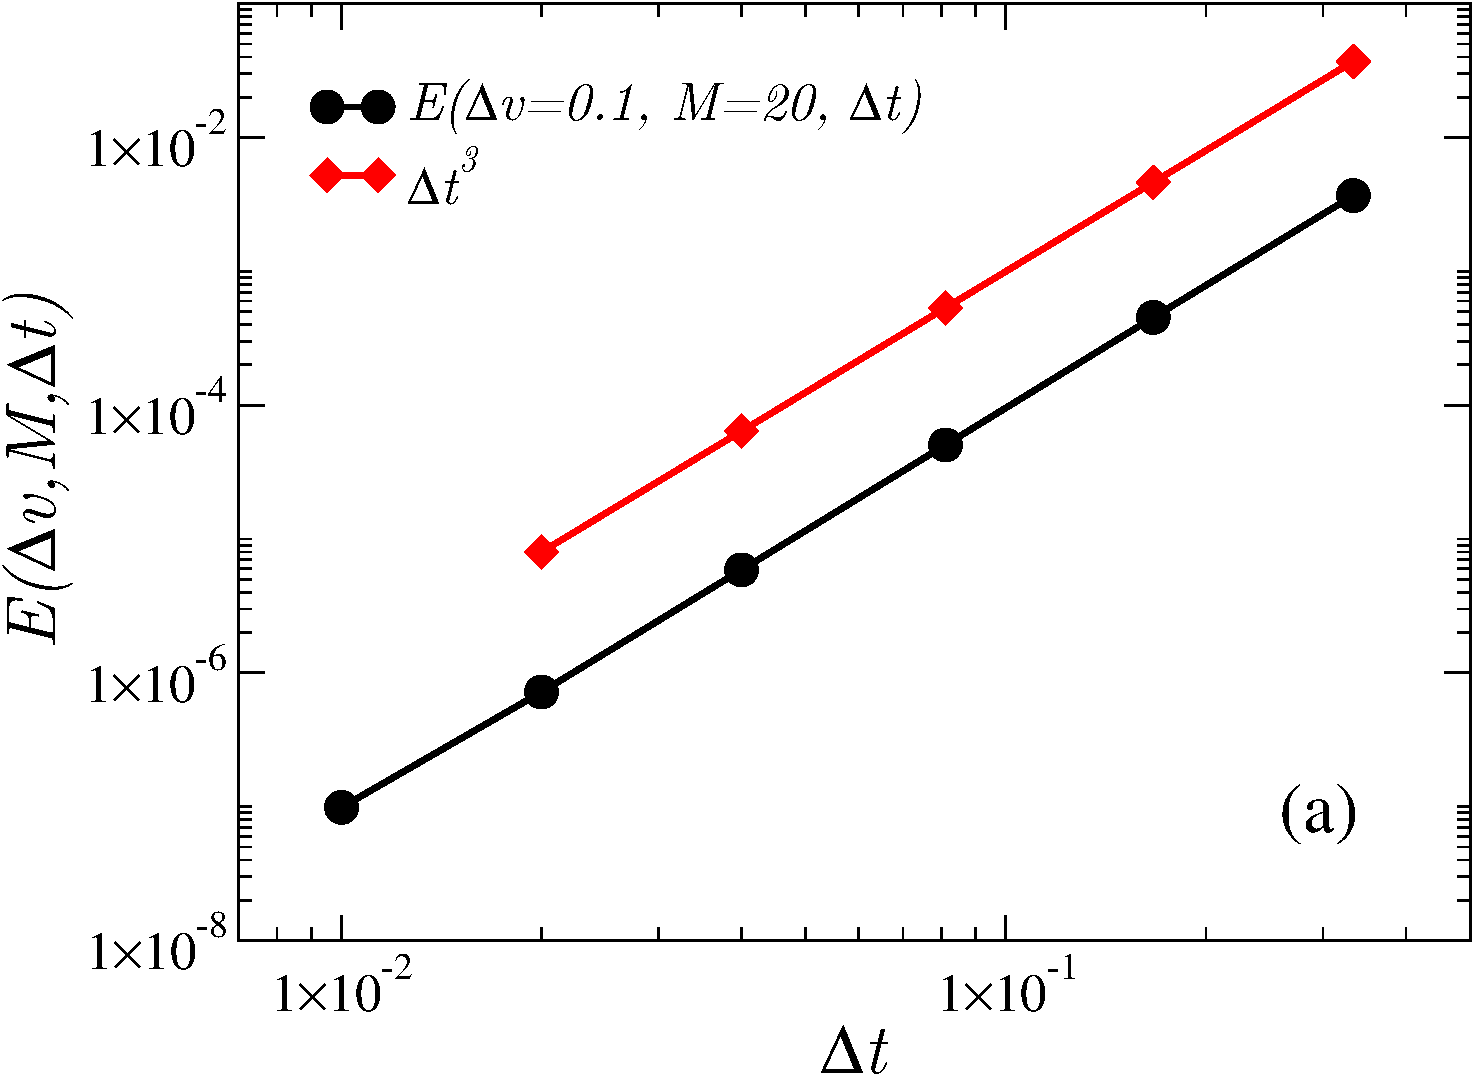
\includegraphics[width=0.45\textwidth]{figuras/errdt.pdf}\\
  \vspace{2mm}
  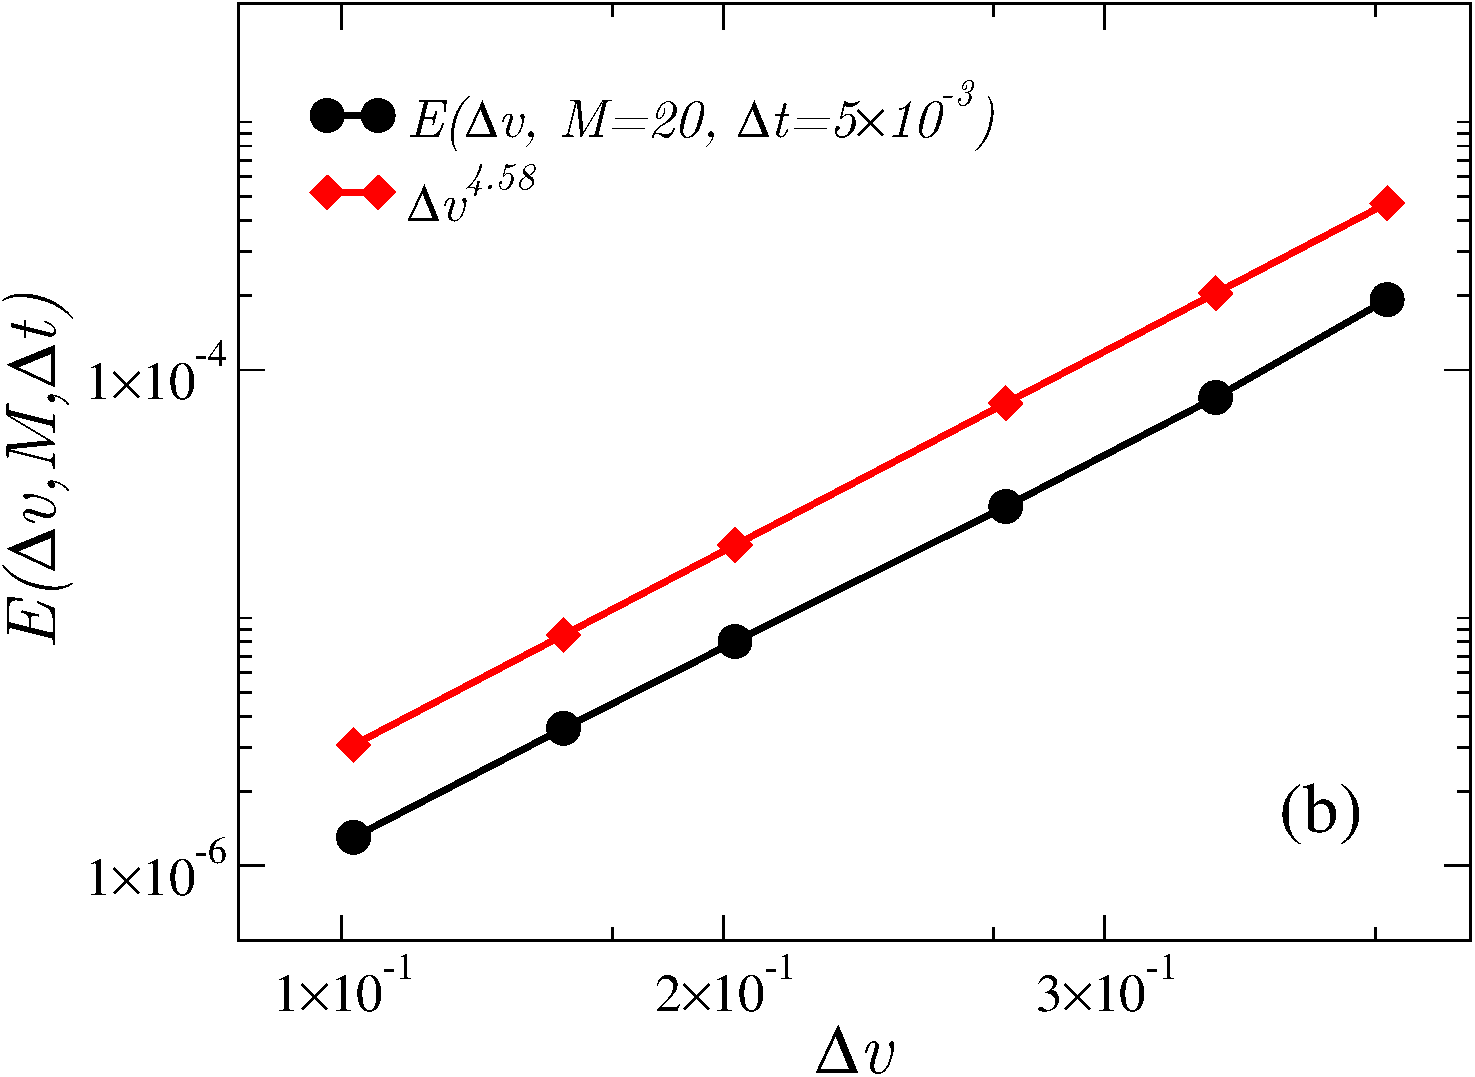
\includegraphics[width=0.45\textwidth]{figuras/errdx.pdf}\\
  \vspace{2mm}
  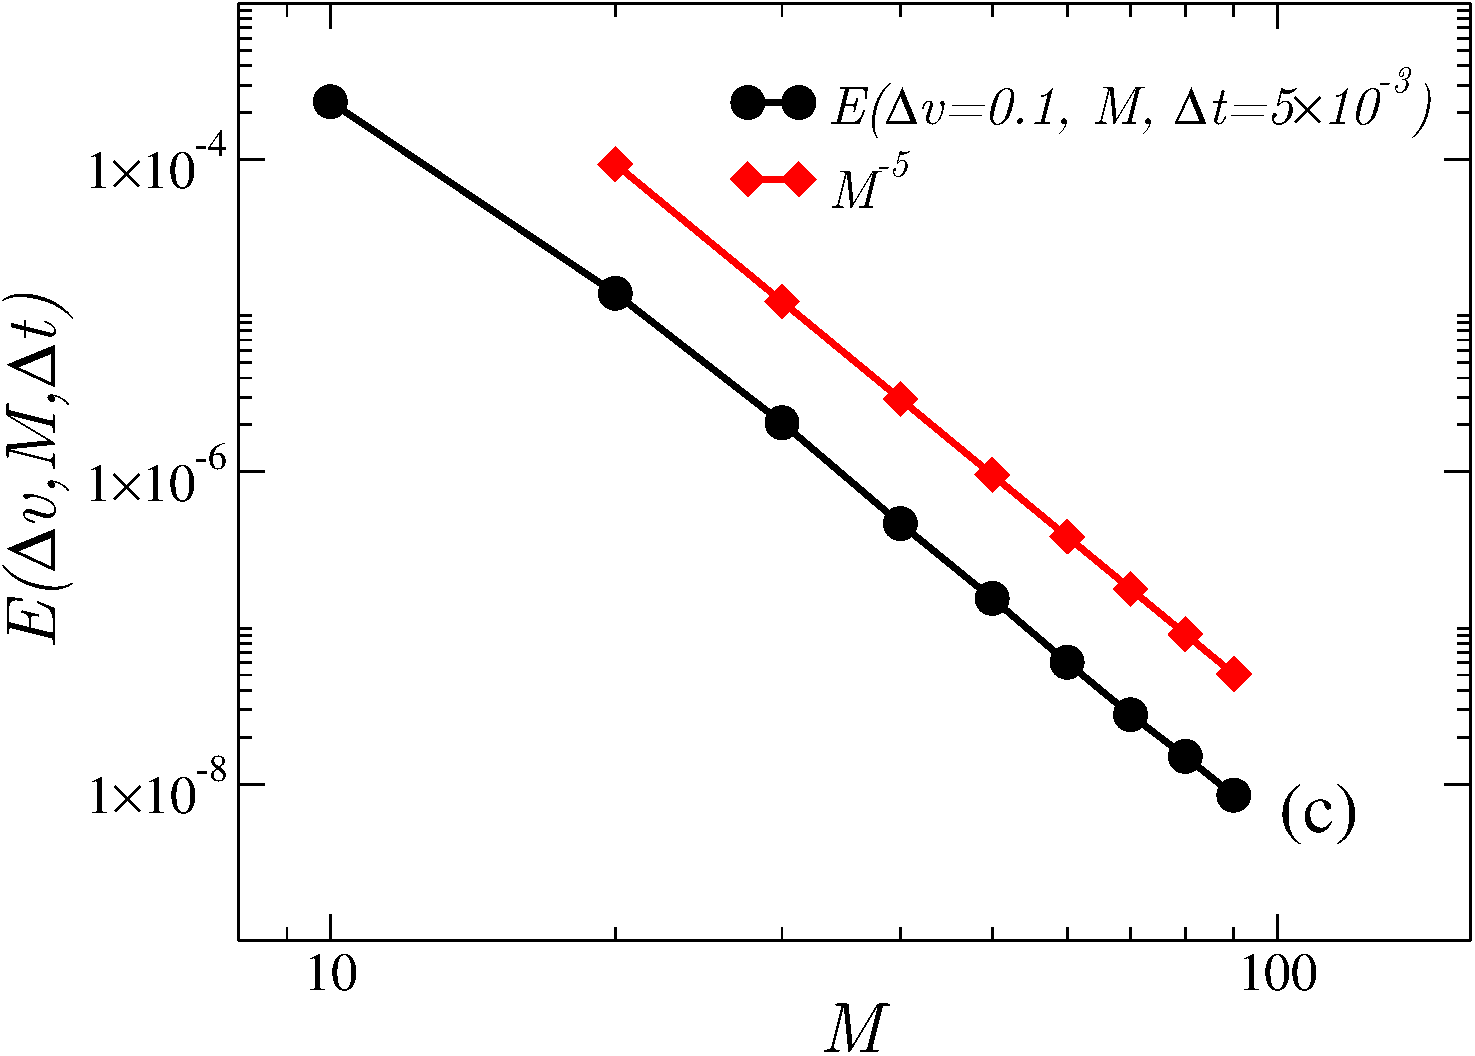
\includegraphics[width=0.45\textwidth]{figuras/xiconv.pdf}
  \caption{En círculos 
  se muestra el error obtenido en diferentes grillas numéricas para el algoritmo 
  propuesto. Las lineas 
  de diamantes indican el orden de convergencia. En el texto se detalla 
  como se determinó el error.}
 \label{fig:conv}
\end{wrapfigure}
\begin{equation*}
\begin{aligned}
 \left[ \id \right. & \left.+ \beta\Delta t\xi_j (2+2\cosh(v)) \ide + \beta\Delta t \mu_t \id \right]  
 u^{n+1}_j  = \\
&\sum_{k=0}^{s-1}\alpha_k u_j^{n-k} + \beta\Delta t \sct
 \sum_{i=1}^{M} w_i \tilde{u}_i^{n+1} + \beta\Delta t q^{n+1},
\end{aligned}
\label{eq:transptd1disc}
\end{equation*}
donde $u^{n+1}_j=u(v,\xi_j,t^{n+1})$, $t^{n+1}=n\Delta t$, con $\alpha_k$ y $\beta$ 
los coeficientes BDF de tercer orden, con $s=3$. El término extrapolado 
a tercer orden viene dado por $\tilde{u}_j^{n+1}=\sum_{\kappa=0}^{2}(-1)^\kappa {3 \choose \kappa+1} u_j^{n-\kappa}$. Nuevamente, 
$\id$ es el operador identidad, mientras qué $\ide$ representa al operador 
de diferenciación espectral obtenido mediante el método de continuación de Fourier. Este procedimiento resulta en una versión implícita 
del método FC--DOM. 


La fig.~\eqref{fig:conv} demuestra las excelentes propiedades de convergencia 
obtenidas mediante el algoritmo propuesto con $\mu_s=\mu_a=q=1$. Dado 
que no se conoce una solución analítica para este problema, 
el error fue obtenido comparando la solución en diferentes grillas, utilizando 
una solución de referencia en una grilla mas finas. El alto orden 
de convergencia obtenido sugiere que los cambios de variables 
propuestos en las variables $x$ y $\xi$ dan origen a grilals numéricas 
adecuadas, capaces de resolver las capas límite involucradas en ambas variables. 
Se definió el error para las figuras~\eqref{fig:conv} (a) y (b) según
  $E(\Delta v, M,\Delta t)=\text{max}_{x,\xi}
    |u(x,\xi)-u^{\text{c}}(x,\xi)|$, donde $u^{\text{c}}(x,\xi)$ 
    es la solución convergida, obtenida en la grilla mas fina. 
Debido a que las diferentes 
    grillas direccionales poseen diferentes abscisas que no coinciden 
    entre sí, para la figura (c) 
    el error fue calculado utilizando el flujo escalar, con  
$E(\Delta v, M,\Delta t)=\text{max}_x |\sum_{i=1}^M w_i u(x,\xi_i)-\phi^{\text{c}}(x)|$.

A continuación, utilizaremos el algoritmo propuesto para 
explorar y demostrar el carácter de las estructuras de capa límite 
consideradas. Por simplicidad, en el resto de esta sección nos restringiremos 
al caso de la ETR independiente del tiempo con soluciones 
obtenidas mediante el algoritmo dependiente del tiempo propuesto, 
dejando a la solución relajar temporalmente, como se describió 
en la sección~\ref{sec:resexp}. Las soluciones resultantes independientes del 
tiempo obtenidas se muestran en las figuras~\ref{fig:blayers1} 
a~\ref{fig:DDlayer}; estas estructuras de capa límite 
existen para todos los tiempos en las soluciones obtenidas 
en el dominio temporal. 

\begin{figure}[h!]
\centering
  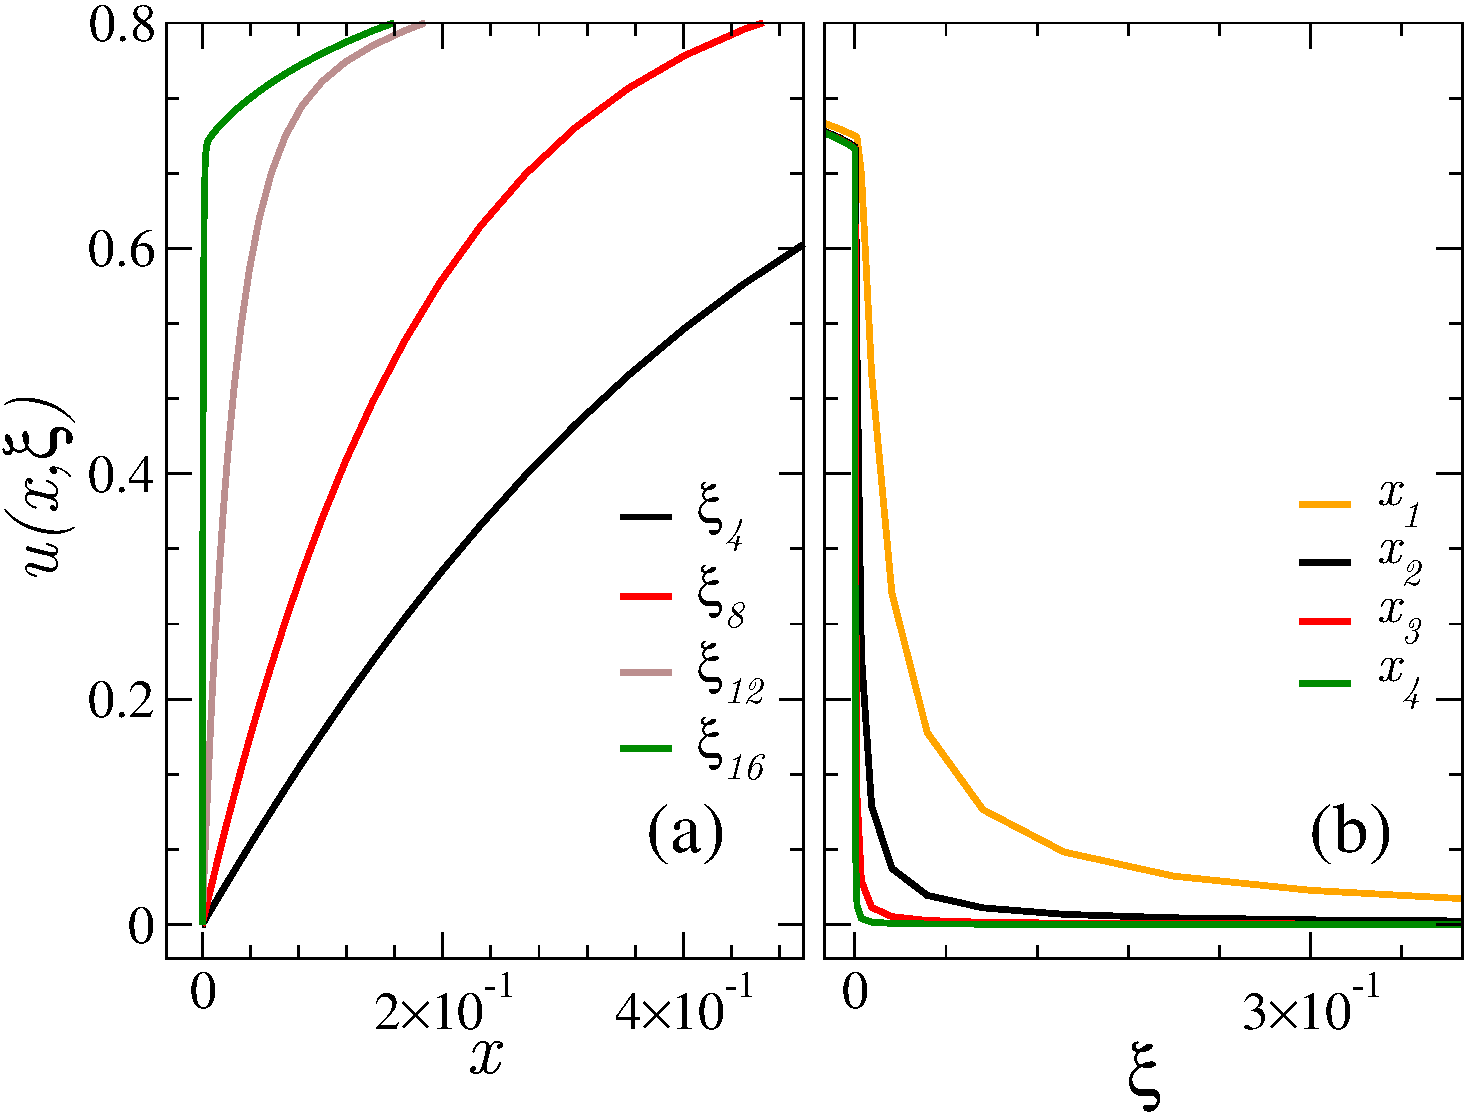
\includegraphics[width=0.5\linewidth]{figuras/xilay.pdf}
  \caption{Capas límite obtenidas como solución 
  de la ecuación~\eqref{eq:transptd} para un entorno de $x=0$ y $\xi=0$, 
  con $\mu_a=\mu_s=q=1$ para distintos valores de $\xi$ y de $x$, 
  con $\xi_i>\xi_{i+1}>0$ y $x_i>x_{i+1}$.}
 \label{fig:blayers1}
\end{figure}
La fig.~\ref{fig:blayers1} muestra las estructuras de capa límite en las 
variables $x$ y $\xi$ con $\mu_s=\mu_a=q=1$ (con parámetros numéricos $N=250$, $M=40$, 
y $-v_{\text{min}}=v_{\text{max}}=25$). Como puede observarse 
en la figura~\ref{fig:blayers1}, los valores mas chicos de $\xi$ 
originan capas límite que se comprimen en regiones espaciales mas 
pequeñas, tal como sugiere el análisis de capa límite realizado 
previamente. 

La fig.~\ref{fig:blayers} demuestra la existencia del fenómeno 
de capa límite incluso para medios altamente difusivos, con 
$\mu_a=q=1$ fijo. En esta figura, se muestra la dirección 
$\xi=\xi_{\text{min}}\simeq 10^{-6}$, para los parámetros 
$N=200$, $M=20$ y $-v_{\text{min}}=v_{\text{max}}=20$. 
Claramente, incluso siendo que para los problemas difusivos 
(donde $\mu_s>>\mu_a$ y $\mu_s>>q$ y $\mu_s>>|x_{\text{max}}-x_{\text{min}}|$~ 
\cite{Larsen1987}) tienden a ser mas regulares en la variable $\xi$ 
---debido a que siendo la dispersión el fenómeno dominante, 
la solución de transporte resulta fuertemente ``promediada'' entre las direcciones---, 
las capa límite que surgen en la variable espacial con coeficiente 
de dispersión creciente tienden a tener pendientes más abruptas 
cuando $x\to 0^+$. De hecho, fue verificado numéricamente que bajo estas condiciones, 
la solución de transporte independiente del tiempo, $u(x,\xi)$ 
para distintos valores de $\xi$ difieren, esencialmente, en la región 
de capa límite.
\begin{figure}[h!]
\centering
  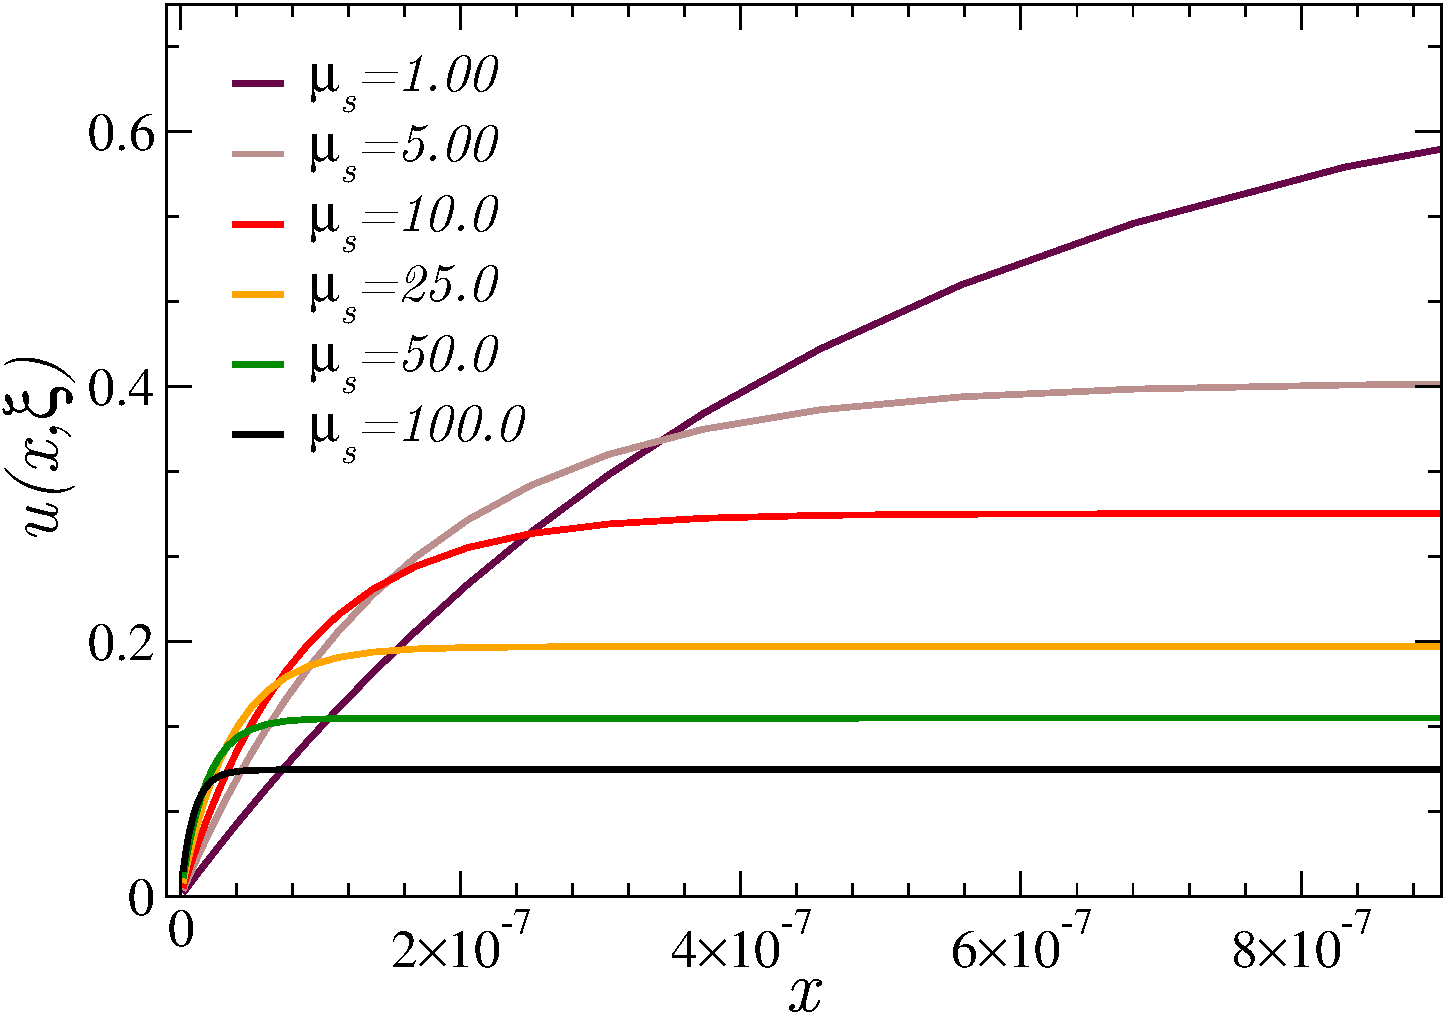
\includegraphics[width=0.5\linewidth]{figuras/blayers.pdf}
  \caption{Capas límite obtenidas resolviendo la ecuación~\eqref{eq:transptd}, 
  con $\mu_a=q=1$ para distintos valores de $\mu_s$. 
  Se muestran las soluciones para la dirección $\xi=\xi_{\text{min}} \simeq 10^{-6}$. 
  Notar las pendientes elevadas que existen para $x\to 0^+$.}
 \label{fig:blayers}
\end{figure}
Han habido esfuerzos en la literatura para comprender un tipo 
de oscilaciones no físicas, originadas 
meramente por un fenómeno numérico que 
surge al resolver la ecuación de transporte 
empleando el esquema de diferencias finitas de Diamante (DD)~\cite{Larsen1987,Petrovic1996,Bal2001}.
En las referencias~\cite{Larsen1987,Petrovic1996} se atribuye 
este fenómeno numérico a condiciones de borde anisótropas, capas límite no difusivas y/o 
a un alto coeficiente de absorción. En esta tesis 
se demuestra la existencia de estas capa límite incluso para el 
caso de condiciones de borde isótropas, y para todos los valores 
de los coeficientes de absorción y dispersión, con una interpretación 
diferente a la reportada en la literatura. En particular, 
nuestra contribución demuestra de forma explícita la existencia 
de capas límite exponenciales, originadas por la imposición 
de las condiciones de borde en conjunto con valores de  $\xi$ 
pequeños, lo cual no fue considerado en las discusiones previas.

Por ejemplo, la referencia~\cite{Larsen1987} trata un problema 
difusivo de transporte (el Problema~1 en dicha referencia) 
el cual, luego de reescalear las constantes, puede formularse 
como an la ecuación~\eqref{eq:transp1d} con $\mu_s=\mu_t=1000$,
 $q=0.1$ y $\mathcal{R}(\xi)=0$. Este es un problema 
 puramente difusivo, con condiciones de borde isótropas, 
 sobre la que dicha referencia afirma~\cite[pp. 317]{Larsen1987} 
 ``...dado que el término de orden dominante en la expansión asintótica 
 de la ecuación de transporte analítica es isótropo, 
 este término no posee una capa límite para este problema''. 
 En contraste, la figura~\ref{fig:DDlayer} muestra que 
 las capa límite estan presentes en este problema, aunque 
 no fueron vistas por el autor debido a que no fueron correctamente 
 resueltas. La solución obtenida por el método FC--DOM implícito 
 con el cambio de variable propuesto que se muestra en dicha figura 
 fue obtenido con $M=40$ direcciones discretas y $N=400$ puntos 
 en la variable espacial. Para la solución obtenida con nuestra implementación 
 del esquema DD se utilizaron $N=10000$ puntos en la fig.~\ref{fig:DDlayer}---
 la cual claramente muestra las oscilaciones espurias producidas 
 por el esquema DD en este contexto.
\begin{figure}[h!]
\centering
  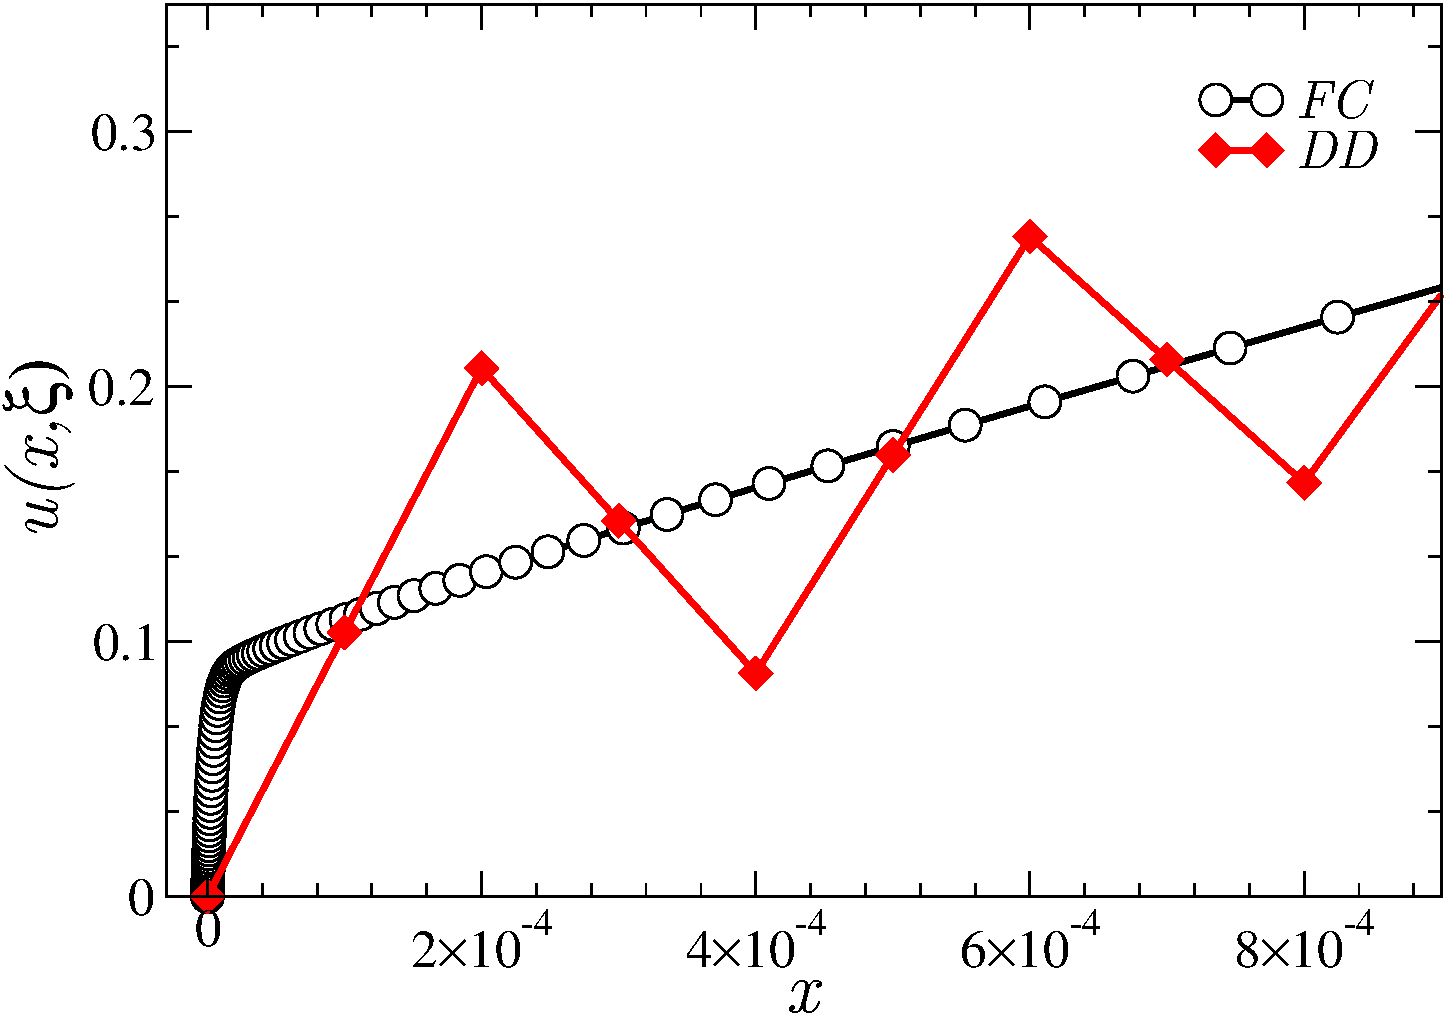
\includegraphics[width=0.5\linewidth]{figuras/layerlar.pdf}
  \caption{Solución $u(x,\xi_{15})$ de la ec.~\eqref{eq:transp1d} 
  con $\mu_t=\mu_s=1000$, $q=0.1$ y $\xi_{\text{15}} \simeq 10^{-3}$
  donde pueden apreciarse las oscilaciones espurias originadas 
  por el esquema DD debido a las pendientes pronunciadas originadas 
  en la capa límite. Se utilizaron $N=400$ para la variable espacial 
  en el método FC, y  $N=10000$ para el método DD.}
 \label{fig:DDlayer}
\end{figure}
En la figura se muestran las soluciones obtenidas por ambos esquemas 
en regiones lejanas a la capa límite, con grillas espaciales variables. 
Puede apreciarse que las oscilaciones originadas por grillas que 
no resuelven correctamente la capa límite tienen efectos en la 
precisión de la solución que se propagan hacia todo el dominio espacial.
\begin{figure}[h!]
\centering
  \includegraphics[width=0.5\linewidth]{figuras/conv_2.eps}
  \caption{Solución $u(x,\xi_{15})$ a la ec.~\eqref{eq:transp1d}, 
  de la fig.~\ref{fig:DDlayer}, para un número variable 
  de puntos en la grilla espacial, lejos de la región de capa límite. 
  Como se observa en esta figura, 
  los problemas numéricos originados por la capa límite en 
  las cercanías del borde 
  en el esquema DD se extienden a todo el dominio espacial.}
 \label{fig:DDlayer2}
\end{figure}

Físicamente, los valores pequeños de $\xi$ para las direcciones 
entrantes en puntos espaciales $x$ cerca del borde (cf. fig.~\ref{fig:parallelgeom}) 
estan asociados a caminos geométricos largos, lo que da origen 
a las transiciones abruptas de capa límite observadas.
Esta estructura de capa límite, que no fue previamente reportada 
en la literatura, constituye un fenómeno físico que no fue correctamente 
descripto, ni caracterizado por varias décadas, y que como se demostró 
en la fig.~\ref{fig:DDlayer} y a lo largo de esta sección, 
posee importantes implicancias en la física y en las simulaciones 
numéricas de los fenómenos de transporte.

En particular, tanto el análisis asintótico de la capa límite que 
derivó en la ecuación~\eqref{eq:intf}, 
así como las pruebas numéricas, sugieren que existirá una capa límite 
siempre qué en un entorno del borde existan fuentes, haya dispersión, 
o condiciones de contorno no nulas. La teoría desarrollada predice 
una capa límite que se desarrollará con gradientes abruptos en regiones 
espaciales $x'$ de orden $x'\sim \ord(\xi/\mu_t(0))$, y en regiones direccionales $\xi'$  
de orden $\xi'\sim \ord(\mu_t(0) x)$. Si las grillas numéricas empleadas no resuelven 
correctamente estas regiones, las soluciones obtenidas para problemas 
que reflejan situaciones realistas para aplicaciones en tomografía óptica 
(y otras disciplinas donde se requiere la solución a la ecuación ETR con 
condiciones de contorno arbitrarias) gozarán de un orden de convergencia 
limitado por la existencia de derivadas no acotadas en el integrando 
colisional, y por la existencia de soluciones subyacentes que en el dominio 
espacial discretizado también lucirán como discontinuas debido a la falta de resolución 
en la grilla numérica, 
con consecuencias e implicaciones similares a las observadas 
en esta sección para la integral colisional en la fig.~\ref{fig:intconvs} 
para la aproximación 
numérica del operador diferencial en la ecuación de transporte. 

Si bien el desarrollo de algoritmos capaces de resolver las capas límite 
en más dimensiones espaciales es un tema de investigación vigente que escapa 
al alcance de esta tesis, los resultados obtenidos en el marco de la misma 
establecen los cimientos para la elaboración de nuevos métodos numéricos 
capaces de hacerlo, de relevancia e impacto en varias disciplinas tecnológicas 
y científicas. 

\pagestyle{empty}


